\chapter{Proton Transfer Reaction Mass Spectrometry}\label{chapter:ptr}
\markboth{PTR-MS}{}

In this chapter, proton transfer reaction mass spectrometry, %(\acrshort{ptrms})
 its underlying chemistry and relevant experimental aspects
are explained.





\section{The PTR-ToF-MS}
As stated in the introduction, PTR-MS is a sensitive technique for real-time monitoring of VOCs in air with a minimal sample preparation. PTR-MS uses hydronium as reagent ion to donate protons to the VOCs present in the analyte gas and detect trace concentrations of targeted compounds.  The KORE Technology Ltd RFIF Mk I PTR-ToF-MS instrument in our laboratory is shown in \autoref{fig:littoral}. 
The main  parts of a PTR-MS instrument and their functions can be simplified to:
\begin{enumerate}
    \item Ion source: production of reagent ions.
    \item Drift tube: protonation and possible fragmentation of the analyte.
    \item Mass spectrometer: detection and identification of product ions.
\end{enumerate}
  These are explained in detail in the following sections.

\begin{figure}%[h]
\centering
\sidesubfloat[]{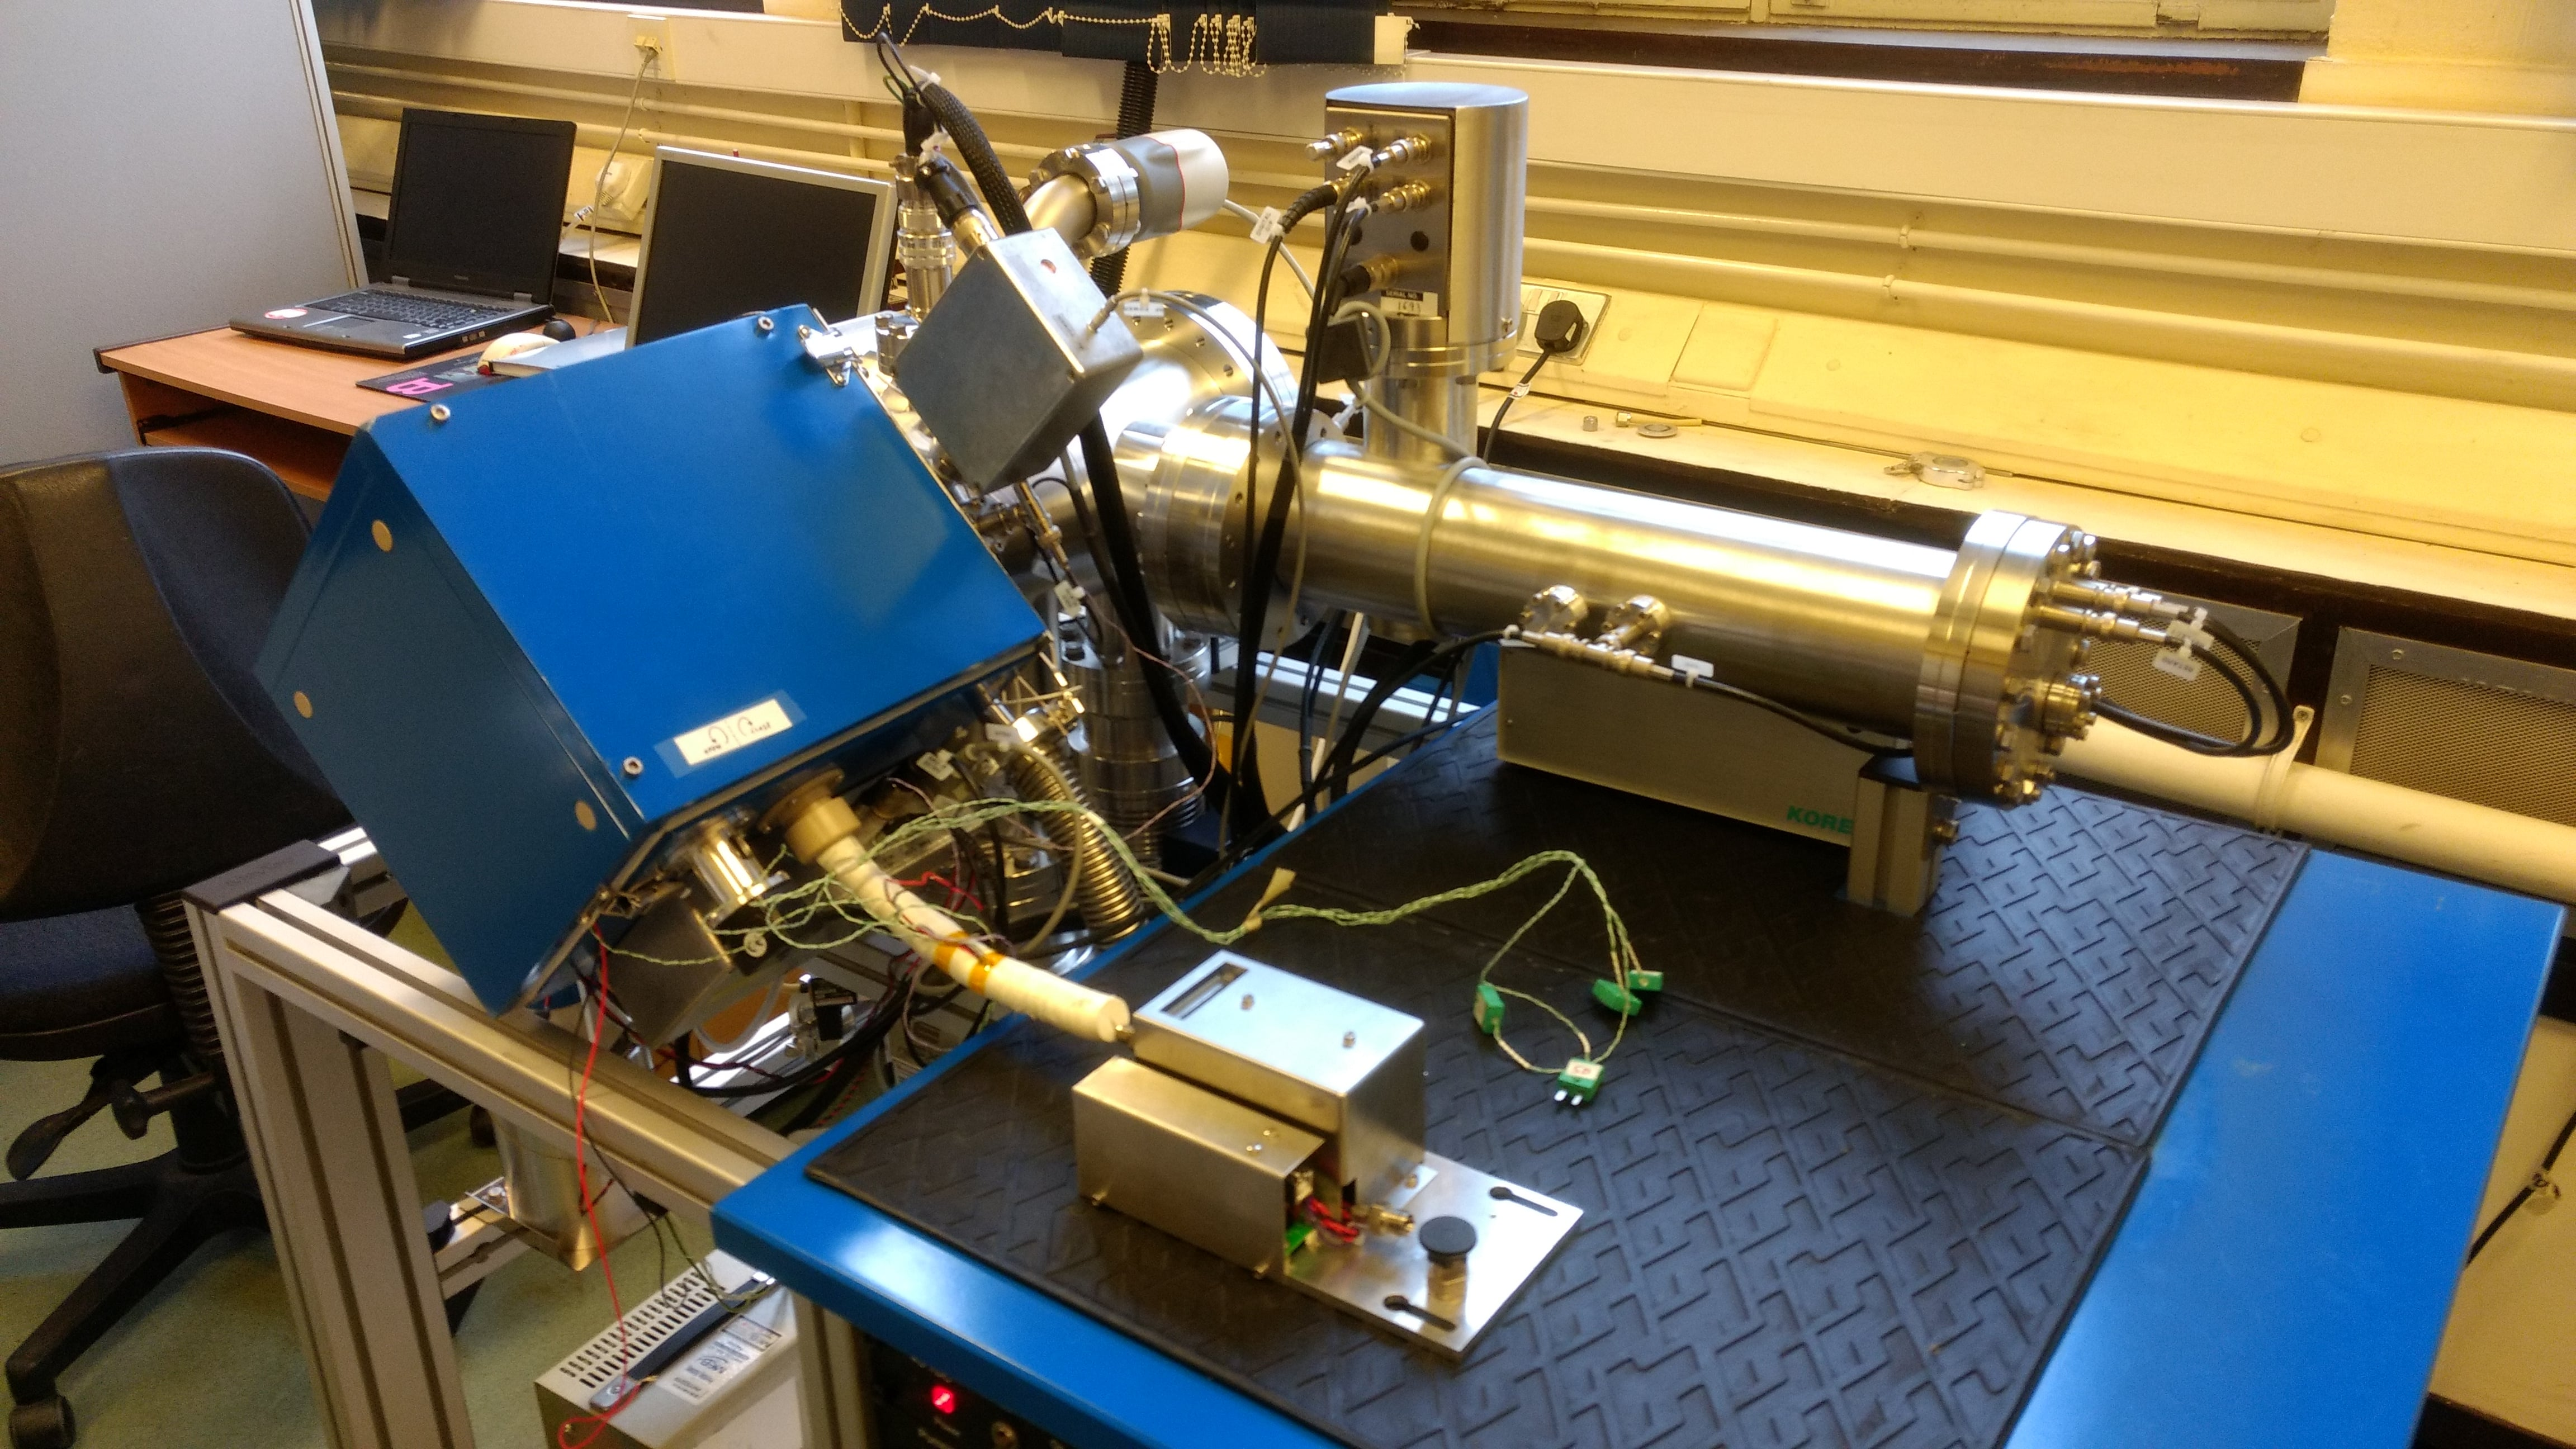
\includegraphics[width=0.9\linewidth]{pics/IMG_20170131_122756718.png}}

\bigskip
\sidesubfloat[]{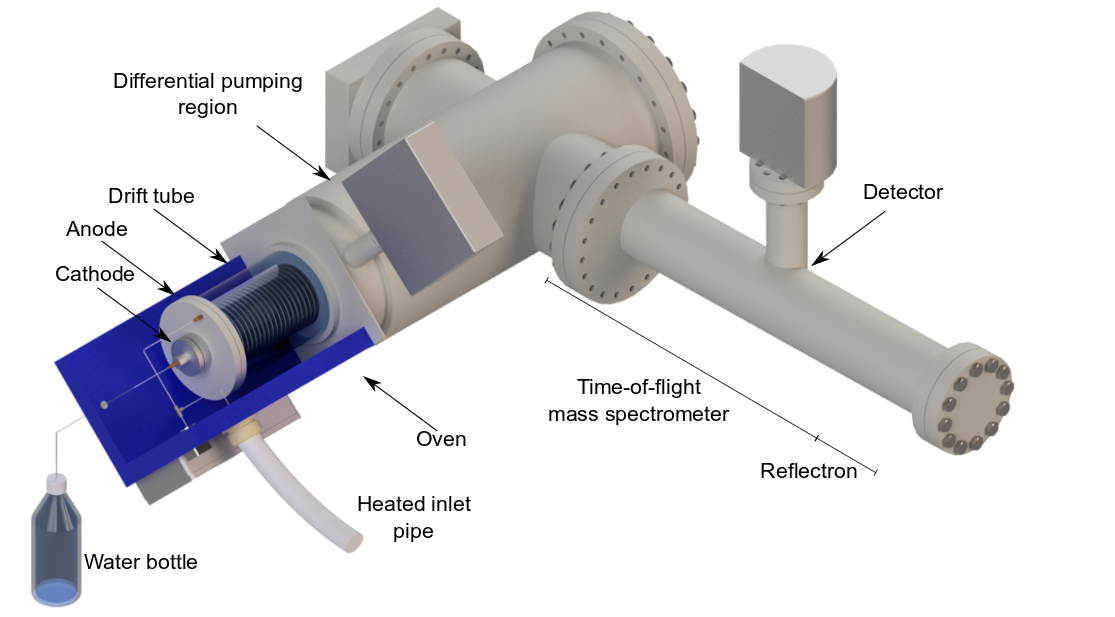
\includegraphics[width=0.95\linewidth]{pics/ptr-ilus.png}}
\caption{(a) Picture of the KORE Technology Ltd RFIF Mk I PTR-ToF-MS  with the TDU attached.  (b) Illustration of the same instrument (not to scale) including the naming convention.}
\label{fig:littoral}
\end{figure}




\subsection{Ion source}
The reagent ions that will ionise the sample are generated in the glow discharge (\acrshort{gd}) %that occurs
in the ion source. Most PTR-MS instruments carry a hollow cathode discharge ion source, to which a voltage is supplied to ionise the gas that flows through it and create the plasma in which the reagent ions are being produced.
%
The cathode in our PTR-MS instrument is shown in \autoref{fig:cathode},
although there are alternatives available like the triple off-axis cathode recently developed by \citeauthor{trion} that  allows to quickly switch from different reagent ion species
\cite{trion}.
%
Note that from now on I will indistinctly refer to plasma, discharge and glow discharge.



%The main advantage of a hollow cathode compared to a planar-electrodes ion source is that in the former higher ion densities can be achieved as the probability that ions hit the ion source's surface generating more ions is higher than in the planar electrode configuration.



\begin{figure}[t]
\centering
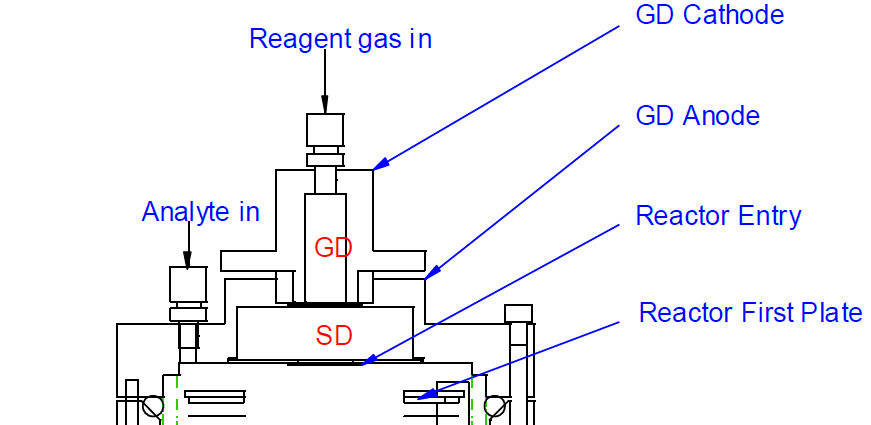
\includegraphics[width=0.6\linewidth]{pics/cathode.png}
\centering
\caption{Diagram of the hollow cathode of the PTR-MS apparatus manufactured by KORE Technology Ltd.}
\label{fig:cathode}
\end{figure}

%\subsubsection{Experimental aspects}







\subsubsection{The glow discharge: production of reagent ions}
Glow discharge is a type of electrical discharge that occur at low pressures (mbar range) and is characterised by a maintained current, ranging from 1uA to 1A, between the cathode and the anode. It receives this name because the ionised gas produces a shining glow whose characteristics depends on the nature of the gas, its pressure and the voltage applied.

During the standard use of the instrument, water vapour is supplied from the water reservoir through a needle valve to the cathode, where H$_3$O$^+$ ions are generated.
The main reaction occurring in the ion source leading to the production of H$_3$O$^+$ from the electrical discharge of water vapour is the first one shown in \autoref{tb:reactions}. It starts when H$_2$O$^+$ has been produced through the electron impact ionisation of water. However, other water fragment ions can also undergo reactions that generate hydronium, following the other reactions shown in \autoref{tb:reactions}. The rate  at which these reactions happen is very close to the collisional  rate.
Furthermore, hydronium ions can cluster to water molecules via hydrogen bonds to form the so-called water cluster ions, i.e. (H$_2$O)$_n$H$_3$O$^+$ with n = 1, 2, 3, ...
Ideally, the formation of these clusters should be avoided to inject pure hydronium into the drift tube.
Otherwise, if the water cluster ions come into play, there are  proton transfer reactions simultaneously occurring in the drift tube with different energies, which makes it more difficult to understand the energetics associated with the different protonation and fragmentation pathways.


The breakdown voltage, which is the voltage difference needed between cathode and anode to start the plasma, is of approximately 750 V for the cathode with the geometry described in \autoref{fig:cathode}.
%
However, after the plasma has started, the voltage difference to maintain the discharge goes down to approximately 350 - 400 V.
%
The anode voltage floats with the voltage of the first plate of the drift tube electrodes, which can be adjusted by the user to set the drift voltage, as will be discussed in the next section. After the glow discharge switch is turned on, it can take the plasma up to a couple of minutes to start.
%Increasing the pressure in the drift tube can assist to start the plasma, as some of the gas in the drift tube will be back-streamed into the cathode and O$_2$ requires a lower voltage to start a plasma.
In our instrument, the ion source pressure is usually between 1 and 1.4 mbar.
%If even with some back-streaming and setting the cathode at high pressure the plasma will not start, cleaning the ion source must be considered.
The plasma struggling to get started or maintained at a pressure  within the common operating range
indicates that the hollow cathode must be cleaned, as an aluminium oxide layer can form inside  and needs to be removed. Another factor that affects the stability of the glow is the temperature of the oven that contains the ion source and the drift tube: %It has been observed that 
the higher the temperature of the oven is, the higher the cathode pressure must be for the glow to be maintained.



%An example of anode and cathode voltages in this configuration would be an anode voltage of 450 volts and a cathode voltage of -300 volts.





\begin{table}[t]
\centering
\caption{Chemical reactions through which hydronium can be produced starting from products of EI of water vapour and their rate coefficients at 300K \cite{doi:10.1002/rcm.1290030312}.}
\label{tb:reactions}
\begin{tabular}{ rcl l }
\toprule
\quad H$_2$O$^+$ + H$_2$O 	&$\rightarrow$& H$_3$O$^+$ + OH  	& k = 1.8$\times$10$^{-9}$\, cm$^{3}$s$^{-1}$ \qquad \\ \midrule
OH$^+$ + H$_2$O  	&$\rightarrow$& H$_3$O$^+$ + O  		& k = 1.3$\times$10$^{-9}$\, cm$^{3}$s$^{-1}$  \\
				& $\rightarrow$& H$_3$O$^+$ + OH		& k = 1.8$\times$10$^{-9}$\, cm$^{3}$s$^{-1}$	  \\ \midrule
O$^+$ + H$_2$O  	&$\rightarrow$& H$_2$O$^+$ + O  		& k = 2.6$\times$10$^{-9}$\, cm$^{3}$s$^{-1}$   \\ \midrule
H$_2^+$ + H$_2$O  	&$\rightarrow$& H$_3$O$^+$ + H  		& k = 3.4$\times$10$^{-9}$\, cm$^{3}$s$^{-1}$   \\
				& $\rightarrow$& H$_2$O$^+$ + H$_2$ 		& k = 3.7$\times$10$^{-9}$\, cm$^{3}$s$^{-1}$	  \\ \midrule
H$^+$ + H$_2$O  	&$\rightarrow$& H$_2$O$^+$ + H  		& k = 8.2$\times$10$^{-9}$\, cm$^{3}$s$^{-1}$   \\ \bottomrule
\\
\end{tabular}
\end{table}



Downstream from the ion source, the ions reach the so-called source drift (\acrshort{sd}) region (shown in  \autoref{fig:cathode}), whose goal is to break the clusters apart before they enter the drift tube. If said clusters are not broken before entering the drift tube, they can also  split up there through collisions with the buffer gas.










\subsection{Drift tube}
The drift tube %(\acrshort{dt})
is the region of a PTR-MS instrument where the protonation and possible fragmentation of the analyte occurs. It is also often referred to as the reactor. A picture of the DT out of the front-end of the PTR-ToF-MS is shown in \autoref{fig:dt}.

\begin{figure}%[h]
\centering
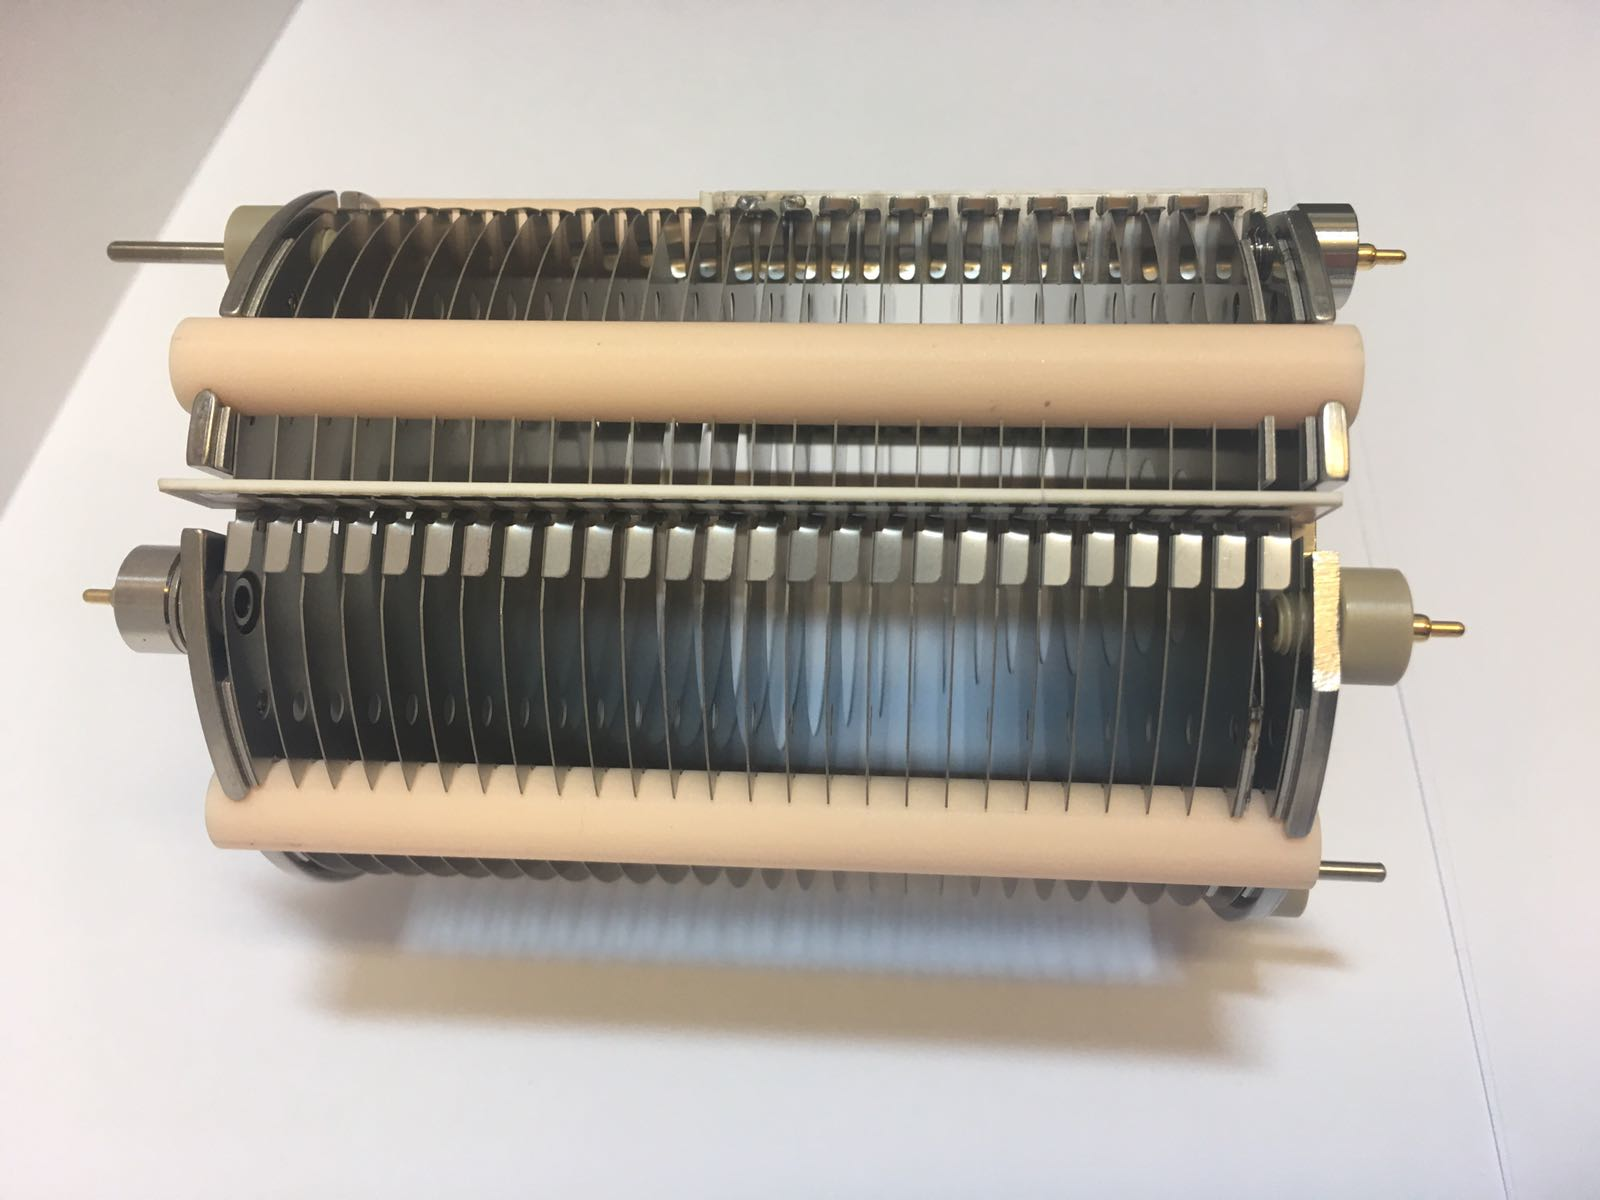
\includegraphics[width=0.6\linewidth]{pics/IMG-20170119-WA0008.png}
\centering
\caption[Picture of the drift tube.]{Picture of the drift tube. Note that in this model the diameter of the electrodes steadily decreases in the second half of the stack.}
\label{fig:dt}
\end{figure}


%\subsubsection{Experimental details}

The drift tube of the KORE Technology Ltd RFIF Series 1 PTR-ToF-MS, whose schematic layout is shown in \autoref{fig:dt_diagram}, consists of 29 stainless-steel ring electrodes of 0.2 mm of thickness with a spacing of 3.2 mm per plate inside a cylinder of resistive glass.
The inner diameter of these electrodes is 40 mm in the first half of the stack and it gradually decreases in the second half to 6 mm.
A 1 M$\Omega$ resistor chain connected to the electrodes allows to supply a linearly decreasing potential to each of them when a voltage is applied between the first and the last plates, generating an electric field in the reactor known as DC field.
When the instrument is operating in these conditions (i.e. without the RF field explained later in \autoref{section:rfif}), we refer to it as working in DC mode or DC-only mode.
% this is repeated in the RF paper

\begin{figure}[t]
\centering
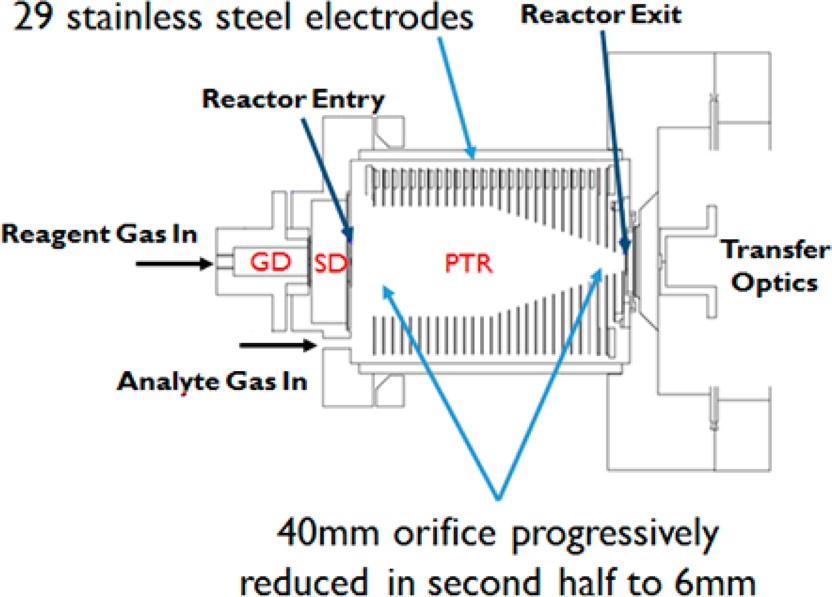
\includegraphics[width=0.6\linewidth]{pics/ac-2016-02982x_0002.png}
\centering
\caption{Schematic diagram of the KORE Technology Ltd RFIF Series 1 PTR-ToF-MS drift tube, together with the glow discharge and the source drift.}
\label{fig:dt_diagram}
\end{figure}

The DC electric field (see \autoref{fig:dt_simion}) drags the ions across the reactor and towards the transfer lenses, where they will get transmitted into the mass spectrometer. As they are drawn through the reactor, ions collide with the neutrals molecules of the background and analyte gases, which can result in protonation and fragmentation of the analyte. The collisional energy can be manipulated by tuning the DC field as well as the reactor's pressure and temperature, whose standard operating values are around 1 mbar and between 100 and 150$^{\circ}$C, respectively, although our oven can reach up to 200$^{\circ}$C.




\begin{figure}[t]
\centering
\sidesubfloat[]{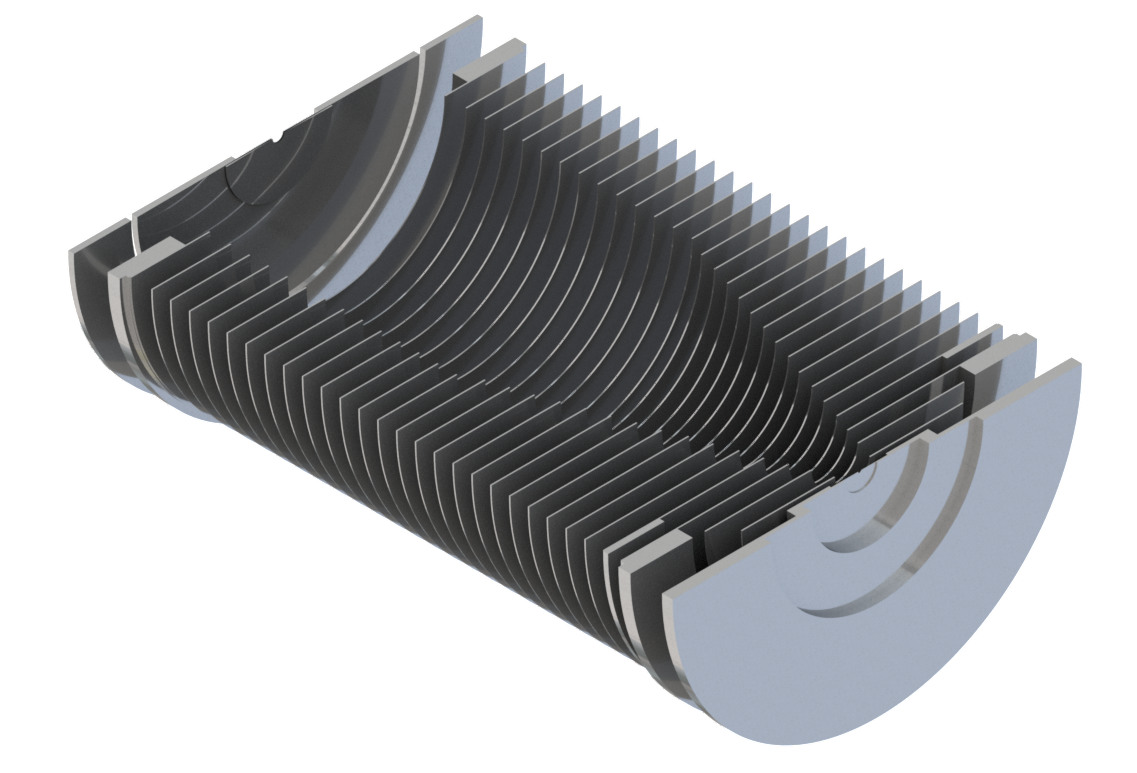
\includegraphics[width=0.4\linewidth]{pics/rfreactorm4.png}}
\sidesubfloat[]{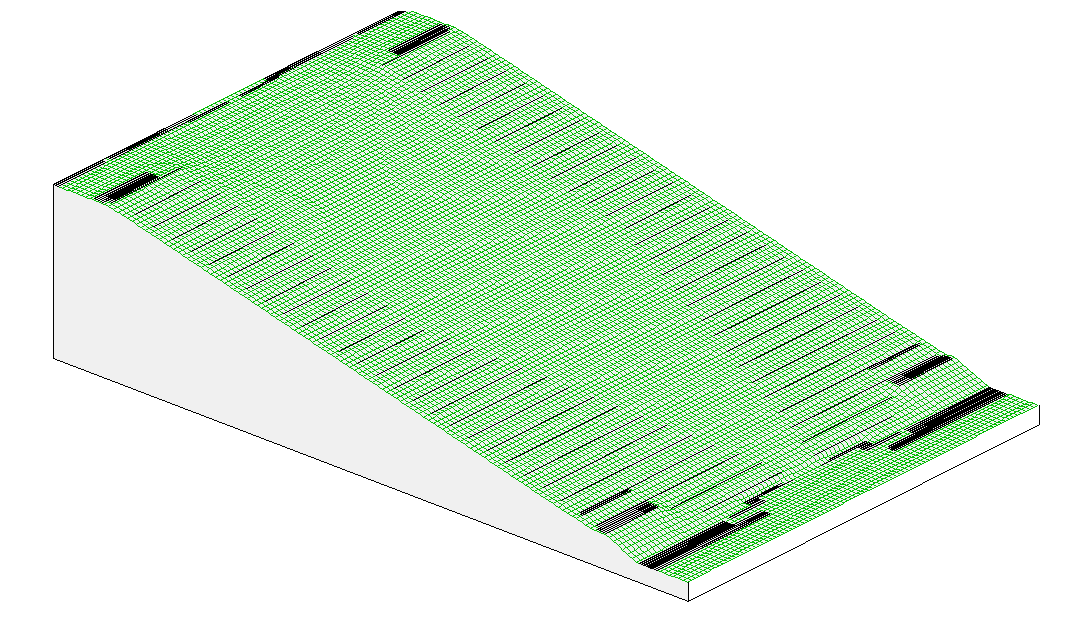
\includegraphics[width=0.4\linewidth]{pics/DC_SIMION.png}}
\centering
\caption{(a) Half section view of the reactor. (b) Potential energy surface of the cross section of the reactor in DC mode calculated in SIMION\textsuperscript{\textregistered} for a random drift voltage.}
\label{fig:dt_simion}
\end{figure}




\subsubsection{Reduced electric field}
As the collisional energy depends not only on the electric field strength (\acrshort{e}) but also on the buffer gas in the reactor, it is convenient to use the reduced electric field (\textit{\acrshort{en}}) as a measure of the collisional energy delivered to the ions.
First, the electric field strength  is defined by the potential difference between the first and the last plate in the reactor divided by its length (\autoref{eq:E}):
\begin{equation}
E = \frac{V_d}{L}
\label{eq:E}
\end{equation}
where \acrshort{Vd} is the so-called drift voltage and it is equal to the voltage difference between the first and the last plate of the reactor, known as PTR Entry and PTR Exit voltages,
that can be adjusted by the user, and L is the length of the drift tube, which is 9.36 cm in our newest instrument.
For instance, a voltage difference between first and last plates of 250 V corresponds to an electric field of 26.71 V/cm.

Similarly, the gas number density (\acrshort{n})  is defined as the number of gas particles per unit volume and can be calculated from the ideal gas equation to be (\autoref{eq:N}):
\begin{equation}
N = \frac{N_A}{V_{mol}}\frac{P_d}{P_0}\frac{T_0}{T_d}
\label{eq:N}
\end{equation}
where \acrshort{na} is the Avogadro's number (6.022$\times$10$^{23}$ mol$^{-1}$), V$_{mol}$ (22414 cm$^{3}$ mol$^{-1}$) is the molar volume of an ideal gas at standard temperature and pressure conditions \acrshort{p0}  and \acrshort{t0}, T$_d$ is the temperature of the drift tube in Kelvin and P$_d$ is the gas pressure in the drift tube in mbar.
For the standard operations conditions of 1 mbar and 100$^{\circ}$C, N is 1.94$\times$10$^{16}$ cm$^{-3}$.
The ratio \textit{E/N} in this case would be 26.71 V cm$^{-1}$/1.94$\times$10$^{16}$ cm$^{-3}$ $\simeq$ 1.38$\times$10$^{-15}$ V cm$^{2}$.
However, it is usual to express the reduced electric field in a different unit called Townsend (\acrshort{td}), which corresponds to 10$^{-17}$ V cm$^{2}$.
Thus, 1.38$\times$10$^{-15}$ V cm$^{2}$ corresponds to a value of 138 Td.
Typically, a PTR-MS instrument is operated between 120 and 140 Td but going as low as 80 Td or as high as 240 Td is sometimes crucial to get a good picture of the dependence of the ion-molecule reactions with the collisional energy.

The ions inside the reactor reach a steady velocity, the so-called drift velocity, \acrshort{vd}, which is proportional to the electric field (\autoref{eq:vd}):
\begin{equation}
v_d = K\cdot E
\label{eq:vd}
\end{equation}
where \acrshort{kk} is the ion mobility, which depends on the ion's mass and structure, and the temperature and pressure in the drift tube, and E the electric field strength.
Note that the product of the ion mobility and the electric field must not be mistaken with the kinetic energy, often referred to as KE.
Also note that the drift velocity does not represent the velocity of an individual ion but an average over the ion cloud, and it can be also  expressed in terms of the reduced mobility, \acrshort{kk0}, and the gas number density at standard pressure and temperature, \acrshort{n0}:
\begin{equation}
v_d = K_0 N_0 \frac{E}{N}
\label{eq:vd2}
\end{equation}
% where K and N are related to K$_0$ and N$_0$ through  \autoref{eq:k0} and \autoref{eq:n0}:

% \begin{equation}
% N = \frac{P_d}{P_0}\frac{T_0}{T_d}N_0			%I am not sure about this equation
% \label{eq:n0}
% \end{equation}

Moreover, the expression for the total mean kinetic  energy of an ion, including both the thermal energy and the energy coming from the electric field, was formulated by \citeauthor{wannier1951bell} \cite{wannier1951bell,wannier1952motion}: % (\autoref{eq:KEions}):
\begin{equation}
    \label{eq:KEions}
    KE_{ion} = \frac{3}{2}k_B T + \frac{1}{2}m_{ion} v_d^2 + \frac{1}{2}m_b v_d^2
\end{equation}
The first term represents the contribution of the thermal energy to the ion's kinetic energy, with k$_B$ the Boltzmann constant and T  the drift tube temperature.
The second term relates to the kinetic energy of the ion from being dragged by the electric field at a drift velocity v$_d$, with m$_{ion}$ the mass of the ion.
Finally, \citeauthor{wannier1951bell} added the last term as the contribution to the ion's kinetic energy  from the randomly-oriented velocity of the ions coming from collisions between the ions and the buffer gas molecules of mass m$_b$, which would be 28.0 or 28.8 g/mol, depending on if N$_2$ or lab air is used as buffer gas.
%
This last term can be used to describe an ``effective temperature'' T$_{eff}$ of the ions according to 
\citeauthor{revercomb1975theory} (\autoref{eq:teff})
\cite{revercomb1975theory}.
%
An estimated drift velocity of 900 m/s at 120 Td and a drift tube temperature of 100$^{\circ}$C yields T$_{eff}$ $\simeq$ 1280 K (i.e. approximately 1000$^{\circ}$C).
%
Whilst this looks like a huge increase in temperature, the ion’s kinetic energy is still way higher.
%
For an ion of \textit{m/z} 100 colliding with N$_2$ buffer gas molecules at 120 Td, the mean kinetic energy would be 0.58 eV, with the contribution from $(3/2)k_{B}T_{eff}$  only being 0.17 eV (i.e. around 29\% of the mean kinetic energy).
%
\begin{equation}
    T_{eff} = T\left(1 + \frac{m_b v_d^2}{3 k_B T}\right)
    \label{eq:teff}
\end{equation}


To properly characterise the energy involved in an ion-molecule collision, the relative energy of the participating bodies must be used instead of the total kinetic energy. This is given by the
%Because the \acrshort{en} is not unambiguously defined, ie different values of P, T and  V$_d$ can yield the same \acrshort{en}.
%Besides the reduced electric field,
the kinetic energy of the collision %of the ion and neutral (analyte)
in the centre-of-mass frame of reference, %\acrshort{kecm} (\autoref{eq:cm}) 
\cite{mcfarland1973flow}:
\begin{equation}
\label{eq:cm}
KE_{CM} = \frac{1}{2}\mu (v_{ion}^2 + v_n^2)
\end{equation}
where µ is the reduced mass of the 2-body system %(\autoref{eq:reduced_mass})%, and v$_{ion}$ and v$_n$ are the ion and neutral velocities, respectively.
\begin{equation}
\label{eq:reduced_mass}
\frac{1}{\mu} = \frac{1}{m_{ion}} + \frac{1}{m_{n}}
\end{equation}
and the kinetic energy of the ion and the neutral are defined by \autoref{eq:KEion2} and \autoref{eq:KT}, respectively:
\begin{equation}
\label{eq:KEion2}
KE_{ion} = \frac{1}{2}m_{ion}v_{ion}^2
\end{equation}

\begin{equation}
\label{eq:KT}
\frac{3}{2}k_B T = \frac{1}{2}m_{n}v_{n}^2
\end{equation}

Combining the expressions above, KE\textsubscript{CM} can be expressed as well as shown in \autoref{eq:cm_final}.
\begin{equation}
\label{eq:cm_final}
KE_{CM} = \frac{m_n}{m_n + m_{ion}} \left( \frac{m_{ion}v_d^2}{2} + \frac{m_{b}v_d^2}{2}\right) + \frac{3}{2}k_BT
\end{equation}
%
where the sub-index $n$ refers to the neutral molecule in both an ion-buffer gas collision or an ion-analyte collision, where only proton or charge transfer will occur in the latter case.
The difference between m$_n$ and m$_b$ for an ion-buffer gas collision is that m$_b$ is an average of the masses of the different species in the buffer gas, while m$_n$ is the mass of the species the ion is colliding with in each collision (e.g. N$_2$ or O$_2$ for lab air, if the rest of the constituents of air are neglected).
It is also important to bear in mind that v$_d$ and v$_{ion}$ are not necessarily the same, as v$_{ion}$ refers not only to the field-aligned velocity.
Note that, as v$_d$ is proportional to the \textit{E/N}, the KE\textsubscript{CM} is quadratic with the \textit{E/N}, as shown in \autoref{fig:KE} for cocaine and 2-butanone, which are two analyte molecules with a considerable mass difference and both are mentioned in this thesis. Their mass difference results in more energetic collisions (10 - 15\%) for cocaine than for 2-butanone.





% I plot these two because there is a big difference in mass and they are mentioned in the thesis.
\begin{figure}[t]
\centering
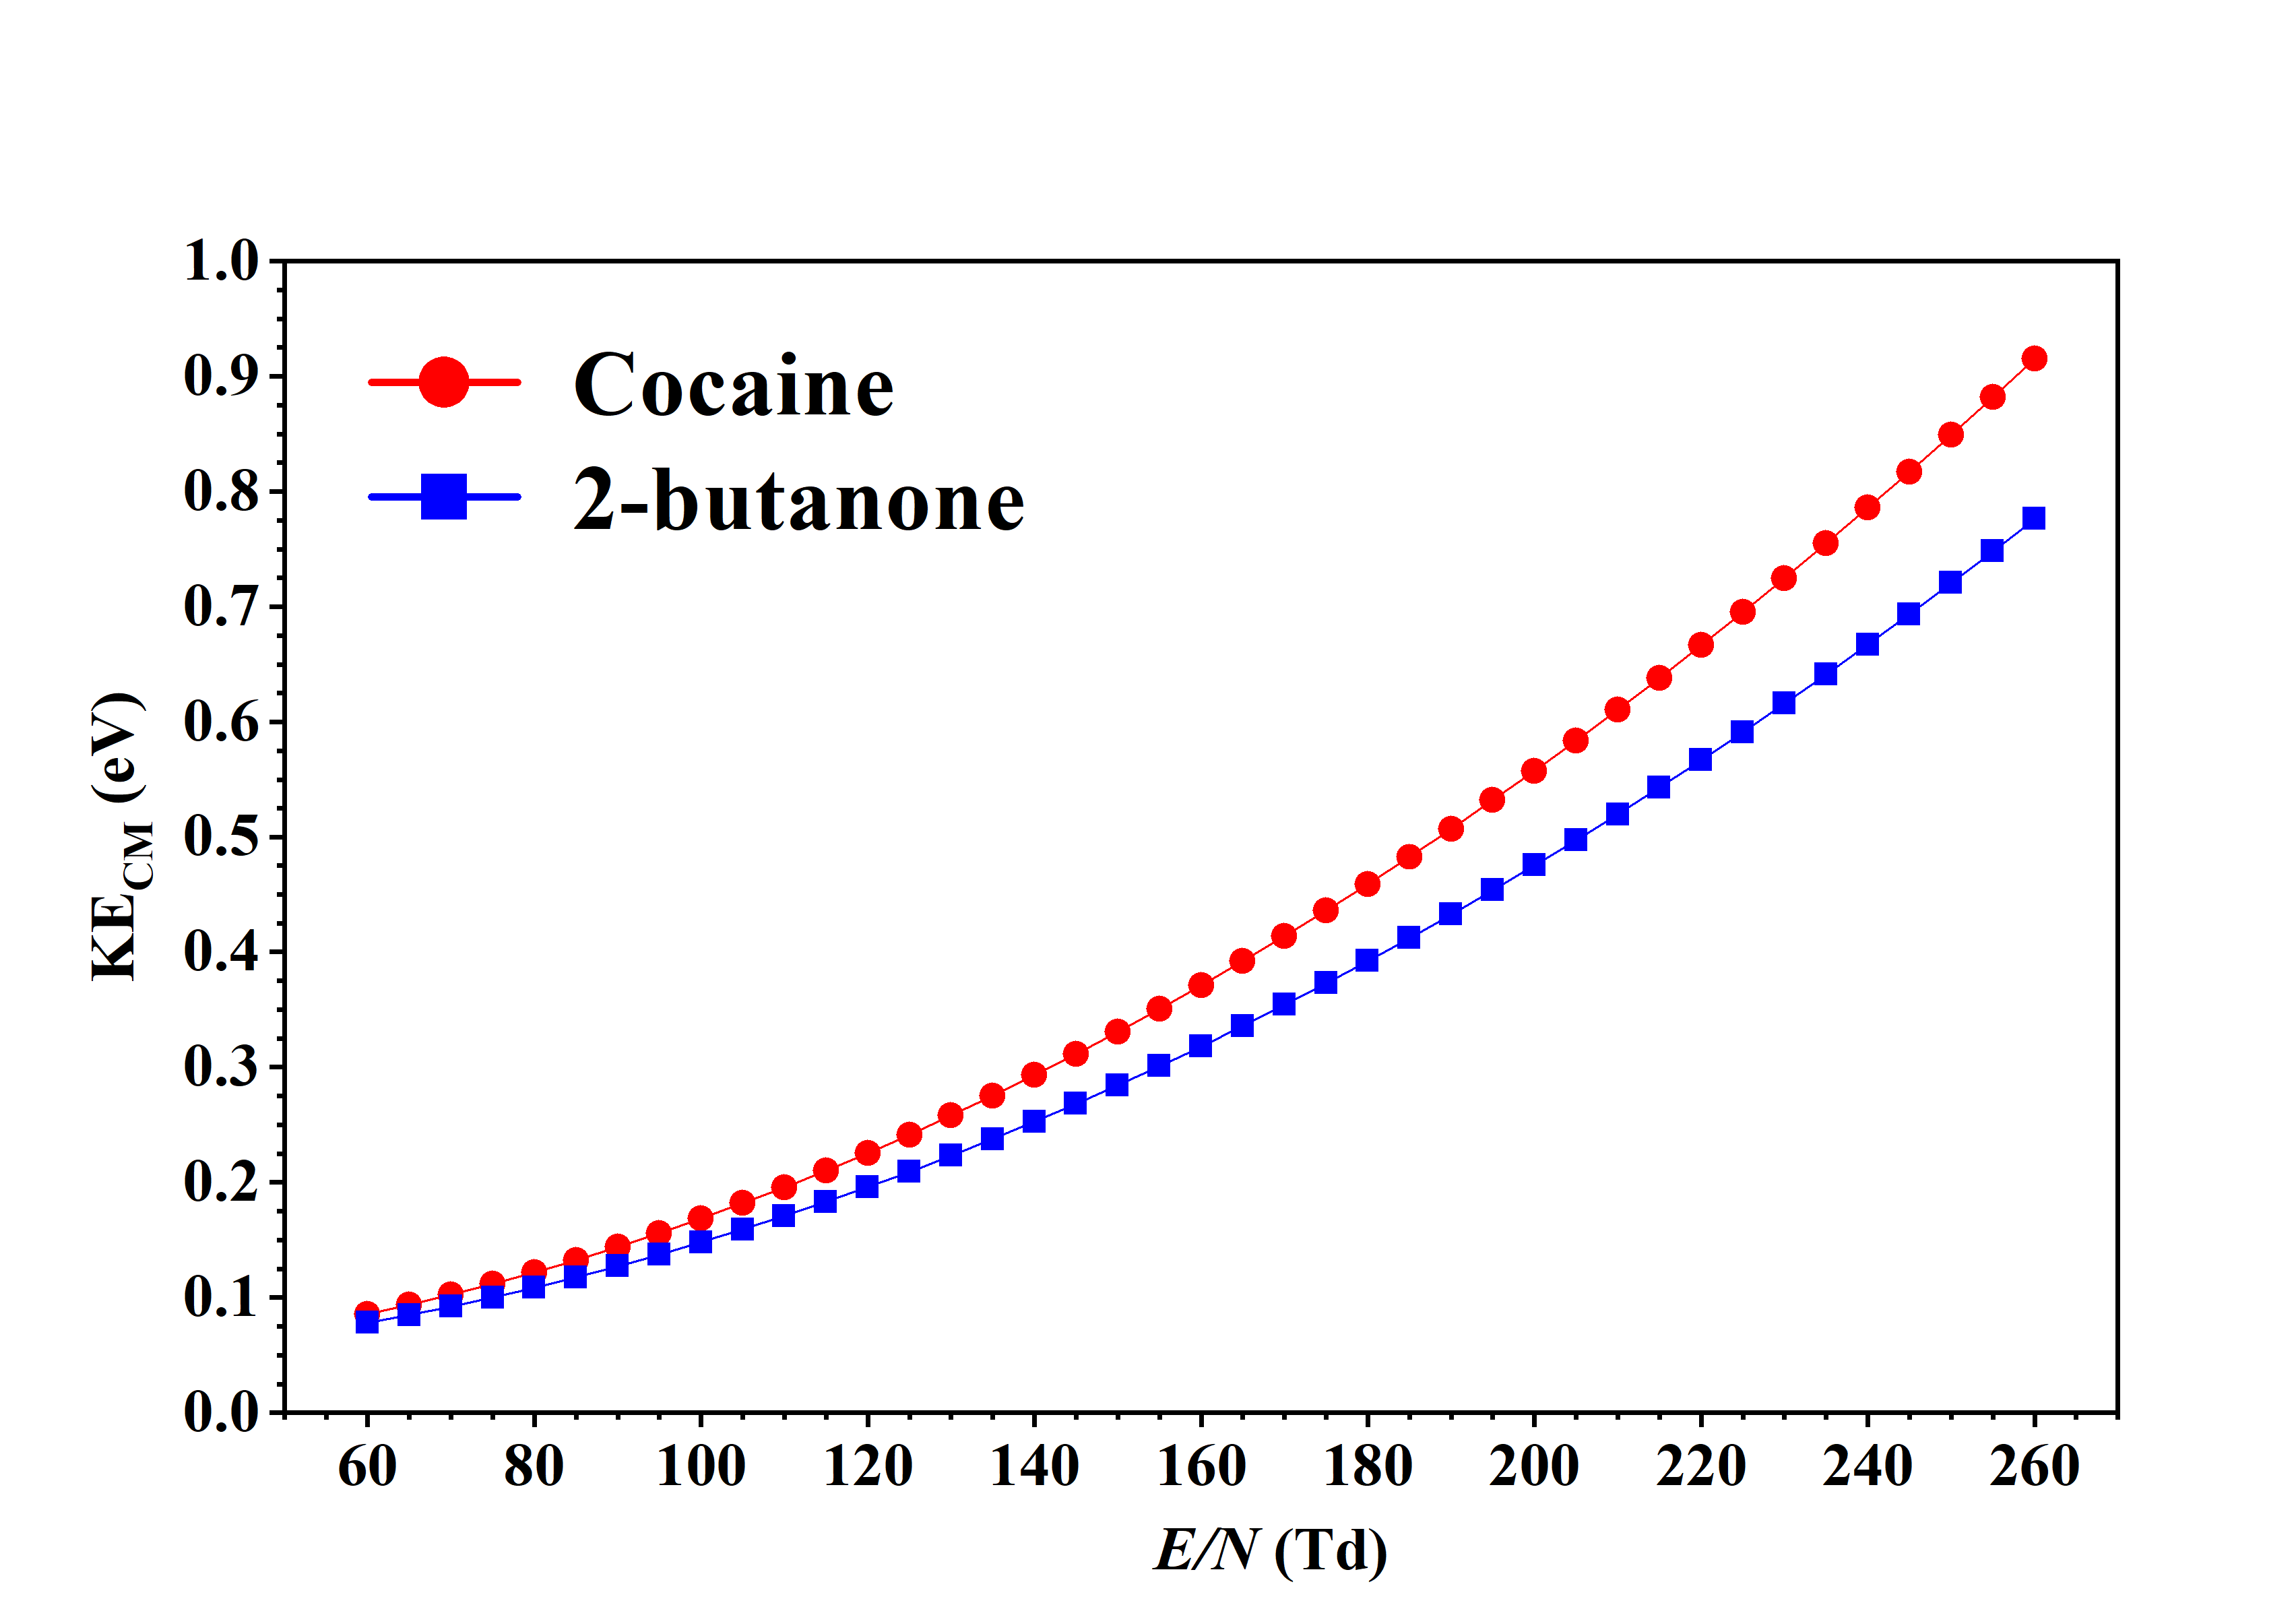
\includegraphics[width=0.7\linewidth]{pics/KE.png}
\centering
\caption{Plot of the kinetic energy of the collision
in the centre-of-mass frame of reference, KE\textsubscript{CM}, as a function of the \textit{E/N} for
collisions of H$_3$O$^+$ with cocaine (C$_{17}$H$_{21}$NO$_4$, 303 g/mol) or 2-butanone (C$_4$H$_8$O, 71 g/mol) at 300 K with N$_2$ as buffer gas. The values for K$_0$ and N$_0$ are  2.8 cm$^2$V$^{-1}$s$^{-1}$ and 2.69$\times$10$^{19}$ cm$^{-3}$, respectively.}
\label{fig:KE}
\end{figure}

















Contrary to the reduced electric field, the centre-of-mass kinetic energy is mass-dependent. %and depends on the ions mobility through their drift velocity.
The centre-of-mass is used rather than the lab reference frame as proton transfer reactions involve inelastic collisions because there is a transference of mass, but still in the centre-of-mass reference frame the sum of the linear momentum of each of the molecules is equal to zero both before and after the collision. % (\autoref{eq:cm2}).
%
%\begin{equation}
%\label{eq:cm2}
%\sum_i \vec{p}_{i,CM} = 0
%\end{equation}
%
Furthermore, the main challenge and source of error when using \autoref{eq:cm_final} is to measure the drift velocity accurately enough. This can be estimated from the ion mobility (\autoref{eq:vd2}) or using the Hadamard transformation \cite{doi:10.1002/rcm.7254}.






Ions will predominantly collide with  buffer gas molecules. \autoref{eq:mfp} gives the expression for the kinetic mean free path (\acrshort{mfp}, $\lambda$) defined as the average distance travelled between collisions, if the colliding particles are considered hard-spheres \cite{hirschfelder1954molecular}.
%
\begin{equation}
    \lambda = \frac{1}{\sqrt{2}N\pi d^2}
\label{eq:mfp}
\end{equation}
%
With d, the so-called kinetic diameter, being  3.64$\times$10$^{-10}$ m for N$_2$ and N = 2.41$\times$10$^{22}$ m$^{-3}$ at 1 mbar and 300 K 
the mean free path is of around 70 µm in the reactor, which corresponds to a viscous flow \cite{ismail2015gas}.
%
This can be compared to the regime in the mass spectrometer, where the pressure is around 10$^{-8}$ mbar and N $\simeq$ 10$^{15}$ m$^{-3}$: the mean free path grows up to the km order of magnitude, becoming much bigger than the dimensions of the chamber. In this case the flow is molecular and the predominant collisions are no longer with other particles but with the walls of the chamber.
%
The transition from the viscous to the molecular regime occurs in the differential pumping region.









%With this estimation, if the length of the drift tube is 9.36 cm, each ion will undergo around 1300 collisions on its way downstream the drift tube.
%However, note that this approximation does not depend on the residence time (or drift time) of the ion in the drift tube as it only accounts for the thermal contribution to the number of collisions.

%It is better to use the collision frequency, knowing that the thermal speed is........
%and hence the collision frequency is....


%knowing that the drift time for a H$_3$O$^+$ ion at 80 Td is approximately 150 µs and at 200 Td it is 70 µs.



%and its drift velocity approximately 900 m/s.

%Also, frequency of collisions.

%Do calculation of collisions per second.
















\subsubsection{Radio frequency ion funnel}\label{section:rfif}
The Radio Frequency Ion Funnel (\acrshort{rfif}) in the reactor of our instrument is a novel piece of equipment %developed by KORE Technology Ltd 
that both delivers extra collisional energy and focuses the ions towards the exit aperture of the drift tube, enhancing both sensitivity and selectivity of the PTR-MS instrument \cite{RF_TNT,barber2012increased}.

\begin{figure}[t]
\centering
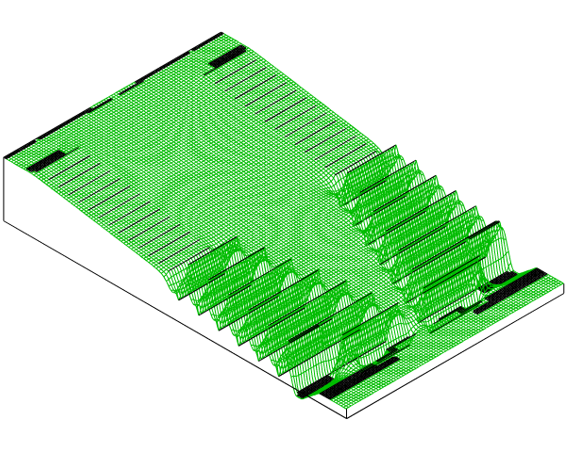
\includegraphics[width=0.6\linewidth]{pics/RF_SIMION.png}
\caption[Potential energy view of the cross section of the reactor in RF mode modelled in SIMION\textsuperscript{\textregistered} with a random DC field.]{Potential energy view of the cross section of the reactor in RF mode modelled in SIMION\textsuperscript{\textregistered} with a random DC field. Contrary to \autoref{fig:dt_simion}, this is a snapshot as the RF field is time-dependent.}
\label{fig:rfif_simion}
\end{figure}
%
%
As mentioned  earlier, in the second half of the drift tube stack the electrode's diameter gradually decreases from 40 mm to 6 mm in a funnel-like configuration. The suitable electronics to provide these funnel electrodes with an RF field are mounted in the instrument. These electronics
%consist of a RLC circuit that
provide the second half of the drift tube's electrodes with a signal of approximately 760 kHz and 200 V peak-to-peak in resonance that we will refer to as RF field (see \autoref{fig:rfif_simion}). At any given time, adjacent funnel plates are supplied with an RF field of opposite polarity. Also, this RF field can be turned on and off in the front panel of the instrument and when it is superimposed to the DC field, which is always on, the instrument is referred to as being operating in RF mode.
%It is also key to properly tune the capacitance from plate 29 to avoid ``closing'' the funnel.
Furthermore, in RF mode the reduced electric field, \textit{E/N}, cannot be used to refer to the collisional energy as in this mode the electric field  in the drift tube is no longer uniform. A comparison of the ion trajectories  in the second half of the drift tube in DC and RF modes is shown in \autoref{fig:rfif_vs_dc} for ions of \textit{m/z} 19 at a drift voltage of 200 V, which corresponds to around 120 Td in DC mode. The funnel effect can be observed on \autoref{fig:rfif_vs_dc}b, which reveals a higher ion density near the exit of the reactor than that in DC mode, even though fewer ions were flown in the RF mode simulations %to reduce simulation times 
because this mode is computationally more demanding than DC mode.
%
\begin{figure}[t]
\centering
\sidesubfloat[]{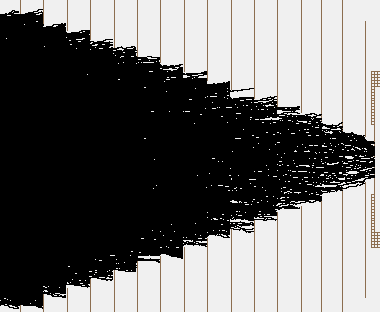
\includegraphics[height=0.23\textheight]{pics/DC_simulation_200V_120Td.png}}
\sidesubfloat[]{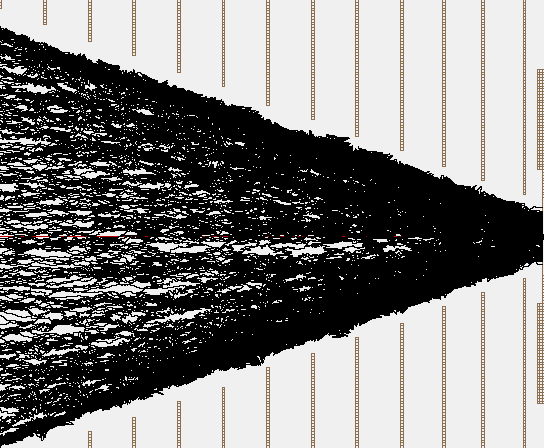
\includegraphics[height=0.23\textheight]{pics/ionfunnel3.png}}
\caption{Simulation of ion trajectories in (a) DC mode and (b) RF mode in the second half of the drift tube for ions of \textit{m/z} 19 at a drift voltage of 200 V (ca. 120 Td in DC mode).}
\label{fig:rfif_vs_dc}
\end{figure}


The ion funnel configuration described in this section is not the only one used in PTR-MS.
%
Others include a short, funnel-like stack of electrodes at the end of the drift tube
%\cite{piel2019airborne}
or 
use a quadrupole enveloping the drift tube
%a resistive glass drift tube that generates a more uniform electric field than the traditional electrode stack, to which an RF field is superimposed from 
\cite{piel2019airborne,krechmer2018evaluation}.



%Besides this design from KORE Technology Ltd, there are other  configurations available in the market.
%For instance, the reactor of IONICON Analytik GmbH instruments can include the so-called \textit{ION BOOSTER}, which is a short, funnel-like stack of electrodes at the end of the drift tube \cite{ionbooster}.
%On the other hand, the approach from TOFWERK consists of a resistive glass drift tube that generates a more uniform electric field than the traditional electrode stack, to which an RF field is superimposed from a quadrupole enveloping said drift tube \cite{krechmer2018evaluation}.


\subsubsection{Fast reduced electric field  switching}\label{section:fs}
Besides the \acrshort{rfif}, another one of the recent hardware developments %from KORE Technology Ltd, this time in conjunction with the \acrfull{dstl}, 
is the fast reduced electric field switching, or just fast switching.
%
It consists of a programmable 500 V power supply unit that can quickly switch the PTR Entry voltage between two preselected values in the range from 50 V to 450 V, which corresponds  to roughly the interval from 10 Td to 250 Td, at a chosen frequency.  This unit can be retrofitted into any other PTR-ToF-MS  from the same manufacturer.
This development has been applied to the detection of different explosives by \citeauthor{doi:10.1021/acs.analchem.7b05211} \cite{doi:10.1021/acs.analchem.7b05211}.
%demonstrated applicable to the detection of explosives %by \citeauthor{doi:10.1021/acs.analchem.7b05211}


A previous \textit{E/N} study of the molecule is needed to identify  the characteristic product ions beforehand. Then the two relevant PTR Entry voltage (i.e. \textit{E/N}) values and the switching frequency are selected.
The lower limit of the switching frequency, while still achieving optimal analytical results, is around 1 Hz.
This limit is a consequence of the time the reactor takes to clear out from product ions at a given reduced electric field, the so-called ``capacitance'', which is typically of around 150 - 200 ms.
The rise and fall times of the voltages given by the power supply unit are not symmetrical, but as these are tens of milliseconds, they get masked out by the capacitance.
%The data obtained  this way is stored in a .lst file
A temporal resolution of 25 ms has been found to be the optimum value %give the best results 
and  also proper data analysis is needed in order to discard the data acquired during the voltage changes.
This is done by means of a script %I wrote in Matlab\textsuperscript{\textregistered}, which is 
described in detail in  section \ref{sec:fs_data}.













\subsection{Differential pumping region and transfer lenses}
When the ions leave the drift tube through the exit plate's orifice, which has a diameter of 400 µm, they enter the differential pumping region, where the transfer lenses are. There is a pressure drop from the 1 mbar range in the drift tube to the 10$^{-4}$ mbar range in the differential pumping stage. This translates into a change in the type of flow, from viscous flow in the drift tube to a molecular flow in the transfer lenses region and further downstream in the mass analyser, 
with %. This means that 
the mean free path of the ions gets bigger than the dimensions of the chamber,
%up to tens or hundreds of meters,
and thus ion-wall collisions are predominant over ion-neutral %or ion-ion 
%collisions.
ones.

The role of the transfer lenses is to focus the ion beam and transport it to the mass spectrometer as effectively as possible. For this purpose, the ion beam is driven through a set of ring electrodes at different voltages. These ion optics focus the ions in the centre of a pinhole in the same way optical lenses do with light. The pinhole helps to clean the beam from chromatic aberrations, which translates into narrower peaks in the mass spectra because the ion beam that reaches the mass analyser is less spatially spread out.
This is qualitatively illustrated in \autoref{fig:tl_simion}.
Also, two pairs of deflectors (not included in \autoref{fig:tl_simion}) can be tuned to steer the beam to maximise the transmission into the mass spectrometer region.

%It is important to note that 
A high potential gradient between exit plate and the first transfer optics electrode can help to increase the transmission but can create a hard extraction of ions, % In the case of a hard extraction, 
 uncontrollably increasing ions fragmentation beyond the exit plate in the early stages of the transfer optics, where the density of ions is still high. This undesired fragmentation can be avoided by setting  the electric field between the exit plate and the first electrode in the transfer optics to no more than a few V/cm. 
 %
 This phenomenon was investigated by Renaud R. Dassonville and I in a series of experiments not included in this thesis that consisted in monitoring the product ions from n-butylbenzene at different extraction and transfer lenses voltages.
 
 %In a series of experiments not included in this thesis, Renaud R. Dassonville and I made sure that in the standard operating conditions of our PTR-MS instruments hard extraction was not occurring. This was checked by monitoring the product ions from n-butylbenzene at different extraction and transfer lenses voltages.

\begin{figure}%[ht]
\centering
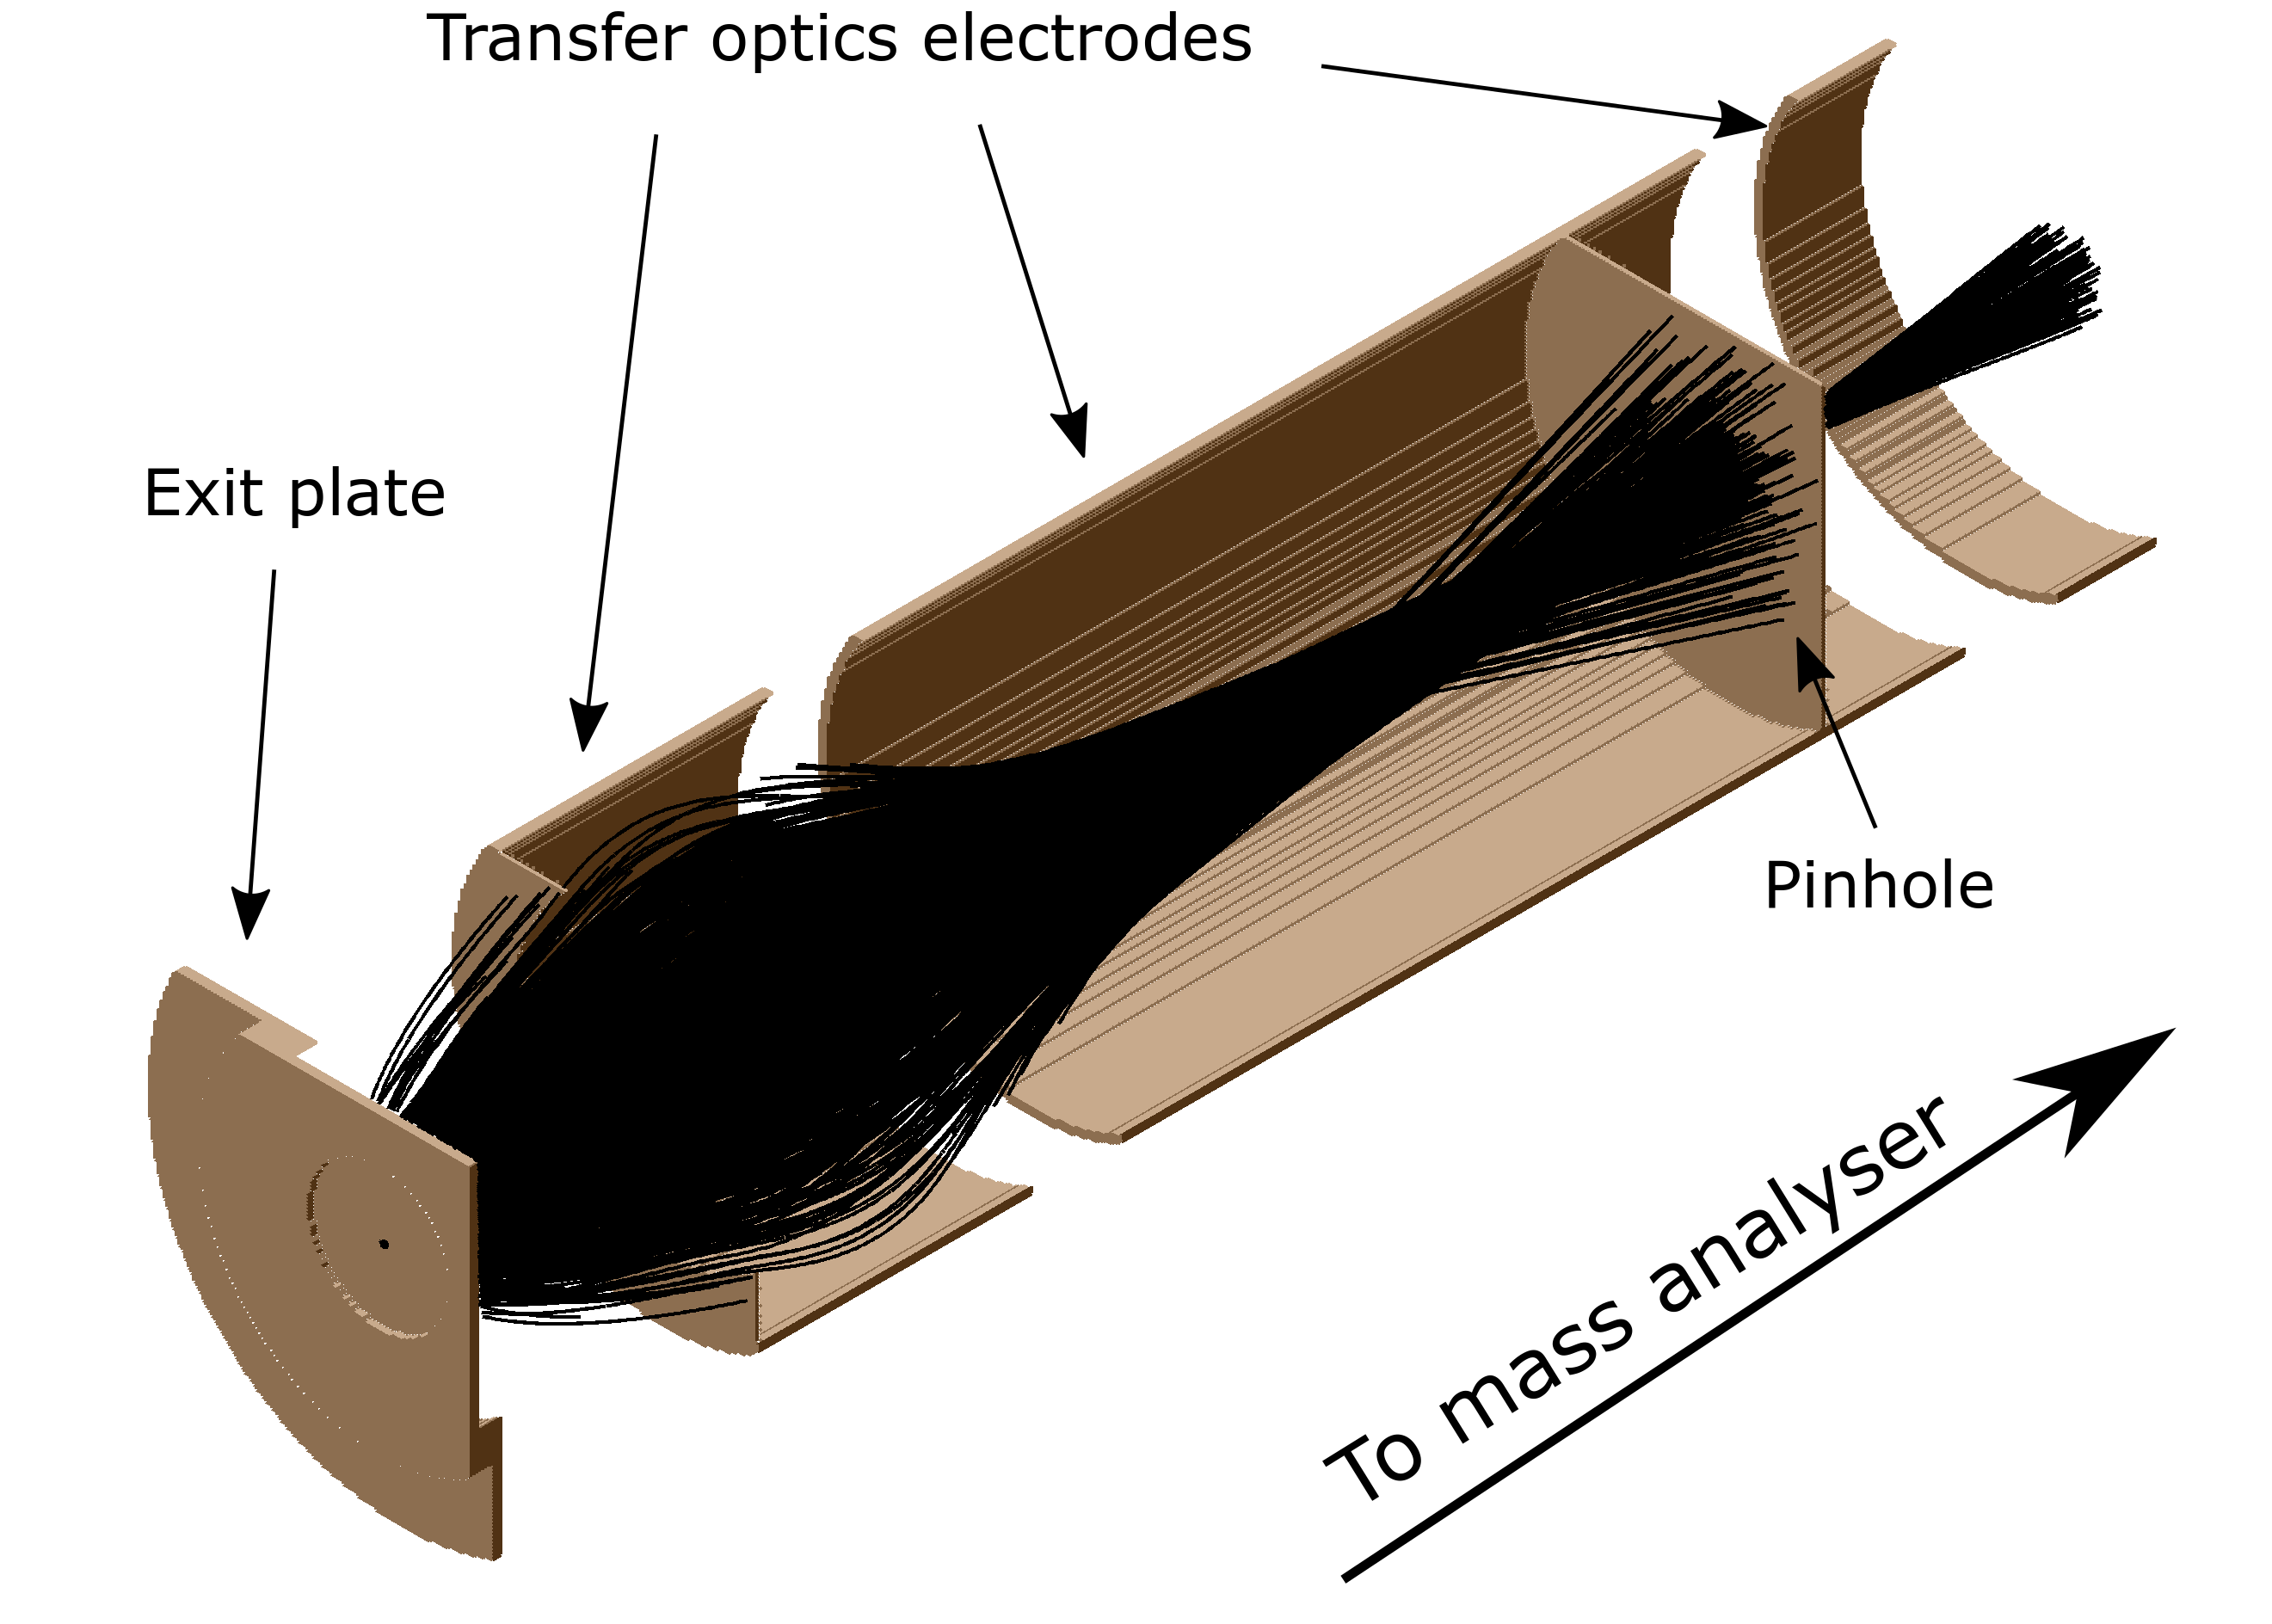
\includegraphics[width=0.6\linewidth]{pics/tf_names.png}
\centering
\caption[Simulation of the ion trajectories in the transfer lens region using SIMION\textsuperscript{\textregistered}.]{Simulation of the ion trajectories in the transfer lens region using SIMION\textsuperscript{\textregistered}. 1000 ions of \textit{m/z} 100 with kinetic energies uniformly distributed between 0 and 1 eV were flown.}
\label{fig:tl_simion}
\end{figure}


\subsection{Mass spectrometer}
The ion beam is transferred from the drift tube to the mass spectrometer (\acrshort{ms}) via the transfer optics. The MS detects the ions according to their mass-to-charge ratio and allocate them in a histogram-like plot mass spectrum.  The terms mass spectrometer and mass analyser will be used interchangeably.

The mass-to-charge ratio is abbreviated to \textit{\acrshort{mz}} and it refers to the ratio of the ions' mass divided by their charge. SI units are not used for the \textit{m/z}. For simplicity, atomic mass units (\acrshort{amu}) are used for the mass (1 amu = 1.66$\times$10$^{-27}$ kg) and the number of fundamental electric charges for the charge (1 e = 1.60$\times$10$^{-19}$ C). 
%Depending on the mass resolution of the MS, \textit{m/z}  is given as an integer (nominal mass) or as a real number (monoisotopic mass).

\subsubsection{Time-of-flight mass spectrometer}
The time-of-flight mass spectrometers  (\acrshort{tofms}, \autoref{fig:tof})  are  the most widely mass spectrometers used in PTR-MS. 
%
Their operating pressure is of 10$^{-7}$ mbar or less.

A ToF-MS works as follows: when ions reach the entrance of the MS (pulser region), a pulsed (tens of kHz) high voltage V of some kilovolts orthogonally repels them towards the other end of the flight tube. Lighter ions will gain more speed than heavier ions, which means that they will reach the detector faster. The time it takes an ion to reach the detector and its \textit{m/z} are related through \autoref{eq:tof2}, which comes from the energy balance in \autoref{eq:tof1}:
%
\begin{equation}
\label{eq:tof1}
qV =  \frac{1}{2} m\left(\frac{l}{t}\right)^2
\end{equation}
\begin{equation}
\label{eq:tof2}
t= \sqrt{\frac{m}{z} \frac{l^2}{2eV}}
\end{equation}
where \textit{m/z} is the mass-to-charge ratio of the ion, $l$ is the length of the flight tube, t is the flight time and $q = e z$ is the ion's charge.
This allows to calculate the \textit{m/z} of the ions as they are being collected at the detector and build the mass spectrum by measuring the ions' time of flight.



\begin{figure}%[ht]
\centering
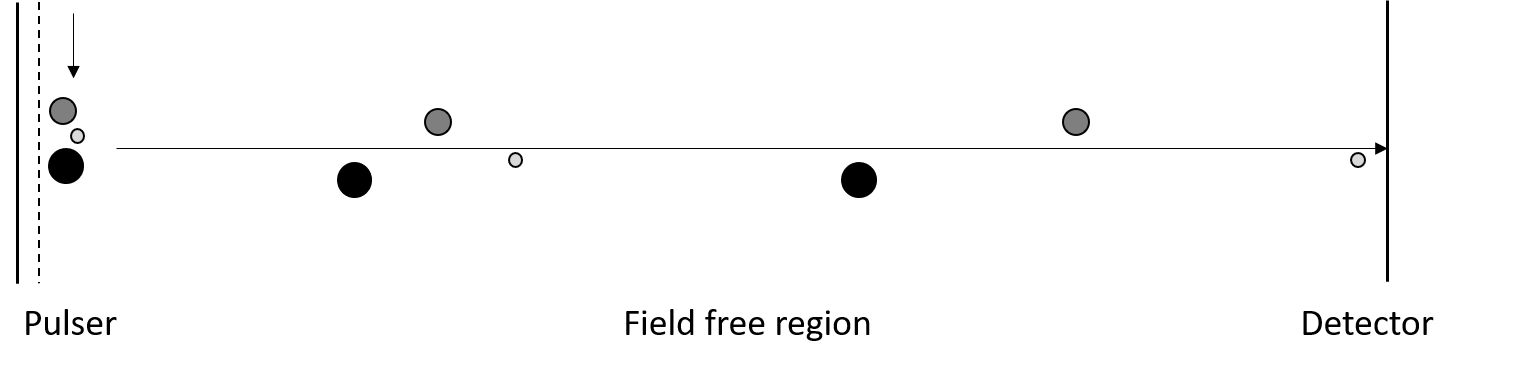
\includegraphics[width=0.8\linewidth]{pics/tofms.png}
\centering
\caption[Diagram of a linear time-of-flight mass spectrometer.]{Diagram of a linear time-of-flight mass spectrometer. Circles represent ions, being their diameter proportional to their mass-to-charge ratio.}
\label{fig:tof}
\end{figure}



\subsubsection{Reflectron}
A spatially spread distribution of ions of the same \textit{m/z} in the pulser region can result in different ion velocities, and hence being detected at different times, broadening the mass spectrum peaks.
%
To amend this a reflectron can be implemented in the flight tube of a ToF-MS.

A diagram showing how a reflectron works is provided in \autoref{fig:tofr}. It basically consists of a series of electrodes with increasing voltage that will reverse the trajectory of the ions. When a cloud of ions reaches the reflectron, ions of the same \textit{m/z} but going faster go deeper in it, having a longer flight distance than slower ions. This way, slow and fast ions of the same \textit{m/z} will reach the detector at the same time, having travelled different distances, yielding narrower peaks and  improved mass resolution. % when the mass spectrum is built.

\begin{figure}%[ht]
\centering
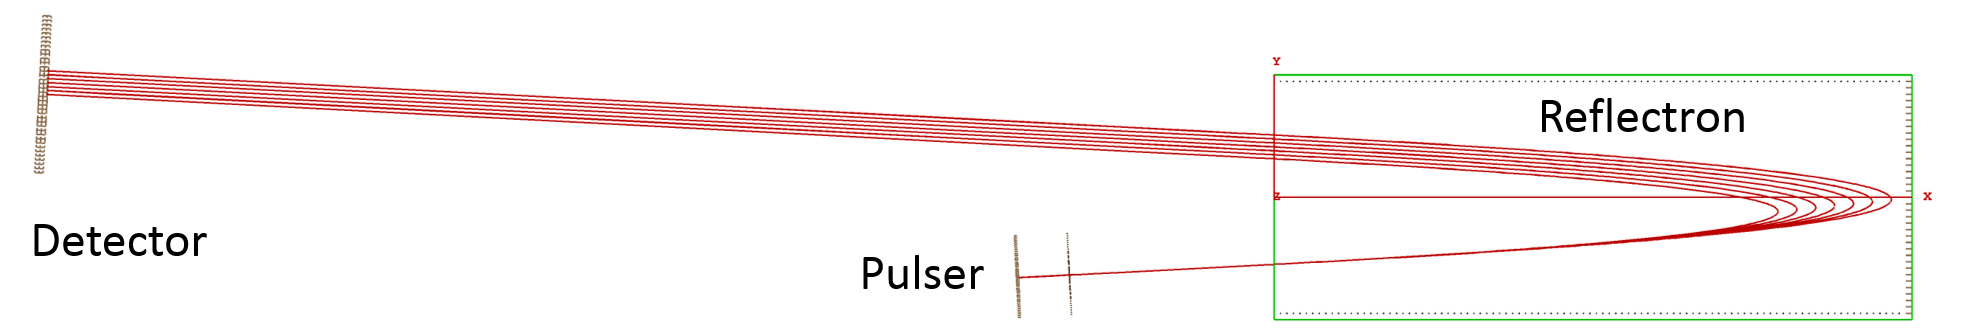
\includegraphics[width=0.8\linewidth]{pics/reflectron2.png}\label{fig:tofr_sim}
\caption{Schematic diagram of a flight tube with a reflectron showing the different trajectories of seven ions of the same \textit{m/z} with different initial velocities simulated  in SIMION\textsuperscript{\textregistered}.}
\label{fig:tofr}
\end{figure}




%\subsubsection{Time-of-flight vs quadrupole}
%Time-of-flight is the most commonly used but it is not the only type of mass spectrometers available for the the  in PTR-MS. Many instruments, typically older ones, use quadrupole instead of time-of-flight technology.


%A quadrupole consists of four parallel rods %(see \autoref{fig:quad})
%from which opposite rods will be at the same electric potential. Said potential is a combination of static and time-dependent fields for which only ions of a certain \textit{m/z} will have a stable trajectory. This allows to select the \textit{m/z} to be transmitted, and these ions will reach the detector at the end of the quadrupole.

%Compared to time-of-flight mass spectrometers, quadrupoles are more compact, robust and cheap. On the other hand, quadrupoles also have some disadvantages. By their principle of operation, quadrupoles need to do a mass scan to build up the mass spectrum. This makes them much slower than time-of-flight devices, which can take measurements in up to 200 ms and are therefore suitable for transient experiments like desorptions. Similarly, the mass resolution of quadrupoles doesn't allow to distinguish between isobaric compounds, which can be done using a time-of-flight mass filter. Also, there is an upper limit for quadrupoles' mass range, which in theory is not a problem in time-of-flight devices although a mass limitation can arise from the use of reflectrons.

%\begin{figure}%[ht]
%\centering
%
\includegraphics[width=0.8\linewidth]{pics/quad.png}
%\centering
%\caption{Schematic diagram of a quadrupole mass filter.}
%\label{fig:quad}
%\end{figure}

\subsubsection{Detector}
Prior to detection, the individual ion signal needs to be amplified to a detectable level. A common pre-amplification setup consists of two microchannel plates (MCPs), which are circular plates of a few millimetre of thickness with an array of tubes that go from one face to the other. These tubes form an angle with the ion trajectory and the second MCP is rotated 180$^{\circ}$ from the first one as shown in \autoref{fig:det} so ions cannot go through without hitting the plates.

Incoming ions are accelerated to $\sim$2 kV before they hit the MCPs' walls. Said MCPs are made of a high resistive material with a secondary electron emission factor greater than one, so that when the incoming ion hits it,  one or more electrons are emitted per collision, generating an avalanche that can amplify a single event by up to a factor of 10$^8$. The cascade electron signal will then reach the anode, where the time-to-digital converter (TDC) will process the analogue signal and convert it into digital.


\begin{figure}%[ht]
\centering
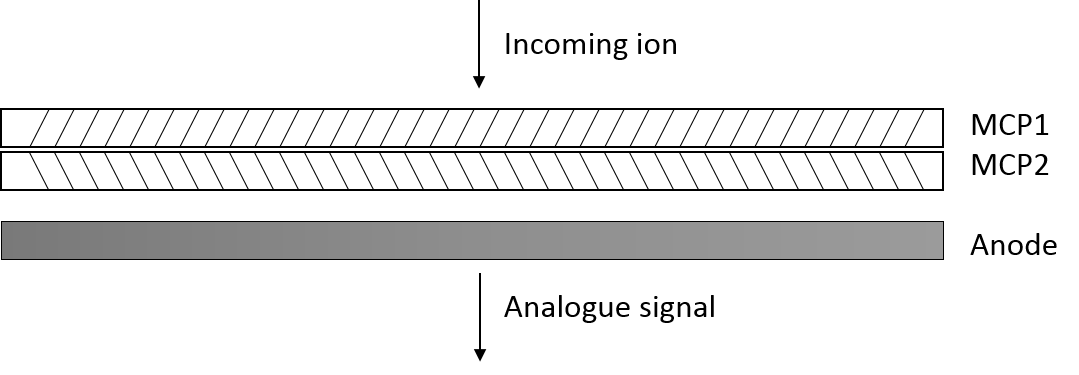
\includegraphics[width=0.6\linewidth]{pics/mcp.png}
\centering
\caption{Schematic diagram of a MCP detector.}
\label{fig:det}
\end{figure}


\subsubsection{Calibration}
As any other scientific instrument, the PTR-ToF-MS must be calibrated before performing any experiment. Note that  this section  refers to calibration as the method to calculate the mass conversions parameters, not the calibration to calculate a concentration from an ion signal. The mass conversions parameters can be calculated by selecting some reference peaks and assigning them their exact \textit{m/z}.
Some peaks that can be used to calibrate the instruments are the $^{18}$O isotope of hydronium (H$_3^{18}$O$^+$, \textit{m/z} 21.023), NO$^{+}$ (m/z 29.998) and  NO$_2^{+}$ (m/z 45.993). 
%
It is also useful to include peaks from the larger end of the mass spectrum (i.e. \textit{m/z} >200). If a single analyte is being studied (i.e. not a mixture), its protonated parent ion can be used.
%It is also useful to use the analyte ion that will be measured as a calibration peak and other peaks resulting from compounds present in air, like protonated acetone ((C$_3$H$_6$O)H$^+$, \textit{m/z} 59.050).
%
The TDC uses \autoref{eq:cal} for this task doing a least squares fitting:
%
\begin{equation}
\label{eq:cal}
m\slash z =  \left(\frac{t-t_0}{C_b}\right)^2
\end{equation}
where \textit{m/z} is the mass-to-charge ratio, t is the ion's time-of-flight, and t$_0$ and C$_b$ are parameters that depend in the mass range the instrument will measure and in some experimental quantities like the length of the flight tube. Note that this equation is the same as \autoref{eq:tof2} for t$_0$ = 0 and $C_b$ = $l/\sqrt[]{2eV}$.



\section{Data post-processing and computational methods}
%In this section I explain how the post-processing of the data is done.







\subsection{Data acquisition, visualisation and treatment}

The analogue data acquired by the PTR-ToF-MS is translated into digital files by \acrshort{tdc} to be visualised and analysed  with the proper software. An experiment can consist in either a static measurement, yielding a stable signal throughout the experiment, or a transient measurement, where the ion signals are time-dependent. These different types of experiments are usually acquired as a mass spectrum  in the form of a Galactic .spc  file from Thermo Fisher Scientific\textsuperscript{\textregistered}, or as a temporal evolution of the mass spectrum, in the form of a binary .lst file, respectively.

As mentioned earlier, a mass spectrum is the histogram-like plot of the counts of detected ions as a function of their \textit{m/z} which, in our case, is stored in .spc files.
\autoref{fig:grams}a shows an example of a mass spectrum visualised with the Thermo Fisher Scientific\textsuperscript{\textregistered}  GRAMS/AI\textsuperscript{TM}  Spectroscopy Software, which is adapted by KORE Technology Ltd to be used with their equipment.
The software does the time to \textit{m/z} conversion following \autoref{eq:cal}.


Transient experiments are stored in %raw files called
.lst files.
 These %are binary
 files  record the timestamp in microseconds of each event in three consecutive bytes in hexadecimal notation, with the most significant byte first, and they are accompanied by a text  (.ini) file containing information about the experiment.
An event can be either the start of a cycle in the detector, always indicated by 0x000000 (i.e. t = 0 µs), or a detected ion (for instance, an ion detected at t = 12500 µs would be recorded as 0x0030D4).
 Therefore an .lst file holds all the information about the experiment and can be plotted as either a cumulative mass spectrum as a function of the \textit{m/z} or as a transient of selected ion signals as a function of the experiment time.
The software GRAMS/AI\textsuperscript{TM} allows to open the .lst files as a mass spectrum, like that in \autoref{fig:grams}a, or as the time-evolution of some particular \textit{m/z}, as shown in \autoref{fig:grams}b. For the latter plot, the so-called regions of interest must be selected before starting the experiment 
to display targeted ion signals. 
%, by selecting the left and right ends of intervals of interest whose ion count will be integrated, displayed and updated as the data is acquired.
%This is  useful in conjunction with the TDU, as it will be explained in the .................... %results section.

%advantage: real time monitoring as the data is recorded



\begin{figure}%[t]
\centering
\sidesubfloat[]{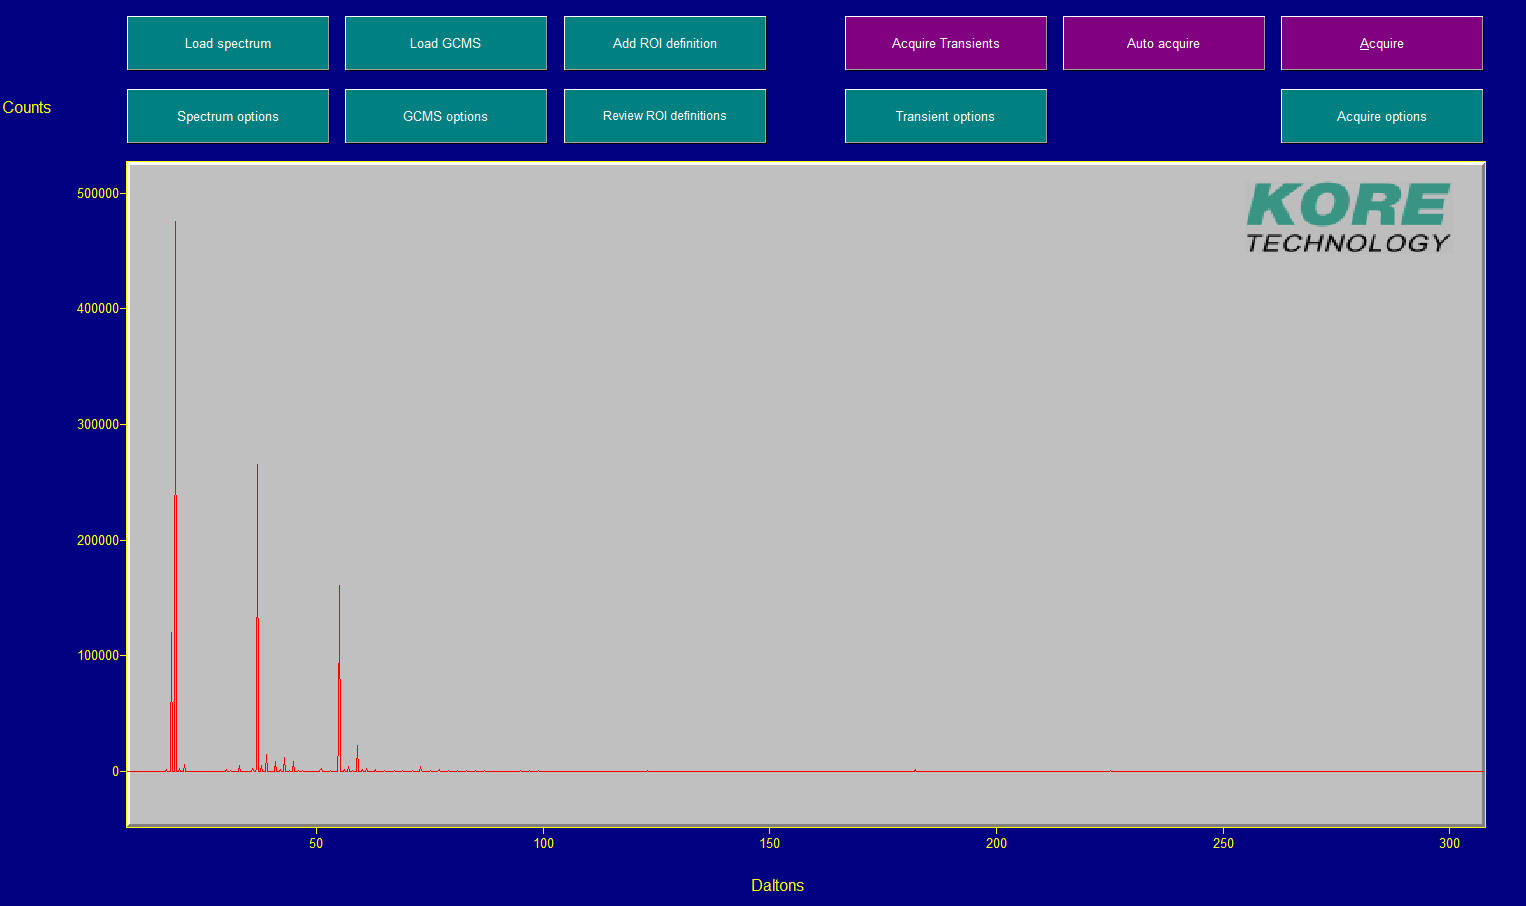
\includegraphics[width=0.9\linewidth]{pics/background_120Td.png}}

\sidesubfloat[]{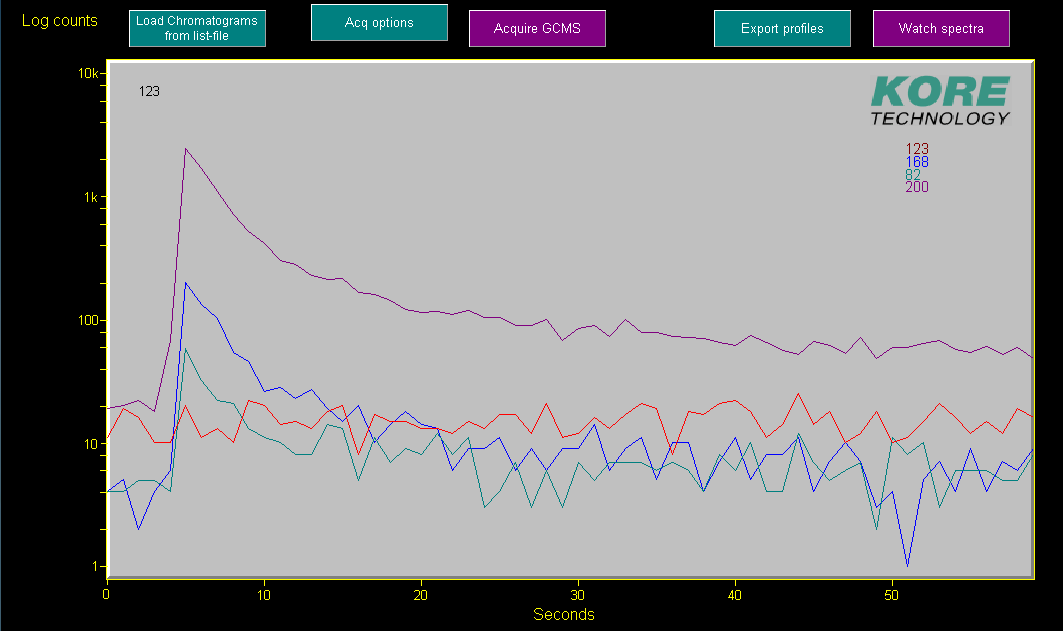
\includegraphics[width=0.9\linewidth]{pics/MeEcg_des2.png}}
\caption{Screenshot of the GRAMS/AI\textsuperscript{TM} user interface for the PTR-ToF-MS instrument manufactured by KORE Technology Ltd showing (a) an example of mass spectrum, and (b) an example of transient experiment data.}
\label{fig:grams}
\end{figure}



Additionally, the Matlab\textsuperscript{\textregistered} command \textit{tgspcread()} is compatible with  Galactic .spc files from Thermo Fisher Scientific\textsuperscript{\textregistered}.
%
This command imports all the fields in the data file into an object-oriented data type called \textit{struct}, which allows quick and easy extraction and manipulation of large amounts of data.
 In the case of the .lst files, the extraction of the data has to be done without help from any library. It is a bit more tedious, as it requires reading the hexadecimal file, building the mass spectra using the parameters stored in the .ini file, do the time-mass conversion and  extract the \textit{m/z} of interest for transient experiments.
 


% With a PTR-MS instrument, a lot of data can be acquired quite quickly so basic programming knowledge comes in handy when dealing with these big data sets.
% One of the best options is to use the Matlab\textsuperscript{\textregistered} command \textit{tgspcread()}, which reads  Galactic .spc files from Thermo Fisher Scientific\textsuperscript{\textregistered}. This imports all the fields in the data file into an object-oriented data type called \textit{struct}, which allows quick and easy extraction and manipulation of large amounts of data.
% In the case of the .lst files, the extraction of the data has to be done without help from any library. It is a bit more tedious, as it requires reading the hexadecimal file, building the mass spectra using the parameters stored in the .ini file, do the time-mass conversion and  extract the \textit{m/z} of interest for transient experiments.
% Using this  as starting point, I wrote my own code to do the data analysis. It extracts all the data from a whole study or experiment to analyse it in Matlab\textsuperscript{\textregistered}, measuring peak positions using the FWHM of the peaks, calculating peak intensities, extracting transient data, subtracting background signals and assigning possible chemical compositions.




\subsection{Calculation of ion intensities}
Once the data is acquired and stored in the files explained in the previous section, it can be analysed and plotted for interpretation, although there are some concerns to %deal with
take into account when doing this.

The counting electronics in the PTR-ToF-MS assumes that each pulse measured at the MCP corresponds to one ion. This can be not true if two or more ions arrive at the detector very close together and their analogue signals overlap so that the TDC translates it as a single event. This phenomenon is known as saturation and happens more often when a high concentration of a compound is being measured.
At a given \textit{m/z}, the maximum number of counts per second the instrument can measure corresponds to the number of cycles per second of the mass spectrometer, which is the number of times the ions are pulsed each second. In other words, at a certain \textit{m/z} only one ion per cycle can be measured. Therefore, a compromise must be found when the experiment is being designed to avoid situations of saturation while getting a suitable signal.
This is given by the rule of thumb that says that saturation occurs when the ion signal at a certain \textit{m/z} is more than 60\% of the cycles per second in the time of flight.
This means that a peak can present saturation effects even before showing a distorted shape. For instance, for a cycle length of 36 µs, the mass spectrometer will be pulsing at a rate of $\sim$27777 cycles per second.
In this case, the 60\% saturation limit would be at an ion signal of $\sim$16666 cps.

%Dead time...........

Peak saturation situations should be avoided when it occurs at product ion peaks, as it can carry other effects like reagent ion depletion.
However, saturation is commonly observed for the reagent ion peaks, whose intensities can be calculated using the suitable isotopes in each case.
%in some scenarios they can be worked around by calculating the ion intensities using the suitable isotopes in each case.
The $^{18}$O isotope peak is used to calculate the reagent ion intensities of  H$_3$O$^+$ or O$_2^+$ as their more abundant $^{16}$O peak is often saturated.
The natural composition of oxygen is $^{16}$O (99.76\%), $^{17}$O (0.03\%) and $^{18}$O (0.21\%) \cite{nistoxygen}.
%This applies to the three most used reagent ions in \acrshort{scims}.
The $^{18}$O isotope is found at \textit{m/z} 21.023 for H$_3$O$^+$ and at m/z 33.994 for O$_2^+$.
However, for NO$^+$ it is better to use the $^{15}$NO$^+$ at \textit{m/z} 30.995 rather than the N$^{16}$O$^+$ at \textit{m/z}  32.002 for two reasons: the $^{15}$NO$^+$  isotope  is more abundant  and also it does not interfere with the  signal of the isobaric compound O$_2^+$  at \textit{m/z}  32.

The $^{13}$C isotope is often used to calculate product ion intensities in saturated peaks and to verify composition assignments if the mass resolution is not enough to distinguish between isobaric compounds.
It is the second most abundant isotope (1.07\%) after  $^{12}$C (98.93\%), with  $^{14}$C is only present at 1 ppt \cite{nistcarbon}.
$^{13}$C is obviously more useful with bigger molecules because normally the bigger the molecule, the more carbons it will have, yielding a peak intensity of more than 10\% at %\textit{(m+1)/z} 
\textit{m/z} + 1 of that at \textit{m/z} for molecules with ten or more carbon atoms.
Of special interest are as well the halogenated compounds containing Cl or Br, which show  very characteristic isotopic  peaks. $^{35}$Cl and $^{37}$Cl are naturally present at abundances of 75.76\% and 24.24\%, while for $^{79}$Br and $^{81}$Br these are 50.69\% and 49.31\%, respectively \cite{nistcl,nistbr}.
Thus,  molecules containing a single Cl atom show a pattern of peaks whose intensity is ca. 3:1 at  \textit{m/z} and %\textit{(m+2)/z}
\textit{m/z} + 2, while for molecules with two Cl atoms this is 9:6:1 at  \textit{m/z}, %\textit{(m+2)/z}
\textit{m/z} + 2 and %\textit{(m+4)/z}
\textit{m/z} + 4. 
For  molecules with a single Br this is approximately 1:1 at  \textit{m/z} and %\textit{(m+2)/z}
\textit{m/z} + 2 while for two Br atoms it is 1:2:1 at \textit{m/z}, %\textit{(m+2)/z}
\textit{m/z} + 2 and %\textit{(m+4)/z}
\textit{m/z} + 4.

With these considerations in mind, for the rest of this thesis when an ion's \textit{m/z} is given with a chemical composition, it will refer to the most abundant isotopologue.
%It is also quite common to show the ion signal in normalised counts per second (\acrshort{ncps}) by normalising the ion signals to 10$^6$ counts of reagent ion signal. For this, the proton affinity of the analyte must be known because proton transfer from the water clusters can also occur and their ion signal must be considered when calculating the ncps. However, in most of this thesis  the data is shown in raw cps to ease the comparison with other instruments, after being usually repeated two times and subtracted the background signal.
In  this thesis  the data is either given in branching percentages (also referred to as branching ratios, BR, or product ion distributions, PID) 
or in raw counts per second, %cps to ease the comparison with other instruments,
after being  repeated two times, averaged and background subtracted.










%depletion

%Another effect to take into account is reagent ion depletion.
%This occurs when the concentration of the analyte is too high
%If the reagent ion signal is depleted, the sensitivity of the instrument is compromised, as there are not enough ions available to protonate (or, in general, to ionise) the analyte.
%It can occur at the same time as saturation for the product ions of the analyte but not necessarily.
%The only solution for this depletion is repeating the experiment with a lower concentration or higher  dilution.





%As stated before, proton donation to the targeted analyte comes from the collisions with the reagent ions, so it is crucial to monitor their signal to know the amount of available protons to be transferred to the analyte.

%The signal of the hydronium and its clusters as a function of the drift tube voltage in both DC mode and RF mode is shown in %\autoref{fig:ri}.
%These agree with the reagent ion signals previously observed \cite{price1977new}.


%The reagent ions' dependence with the voltage in DC mode is very different to that in RF mode. In DC mode the clusters break apart as the drift voltage increases. On the other hand, the RF field in RF mode delivers an extra collisional energy that breaks the clusters apart independently of the drift voltage. Also, this RF field can create potential wells for the lighter masses generating a low-mass cut-off of the transmission \cite{Chung123}.

%The measured reagent ion signal depends on the clustering/declustering reactions and the transmission of the instrument. Furthermore, clustering depends on humidity, collisional energy (E/N) and drift time. The higher the pressure in the cathode, the more hydronium is produced but it also will tend to create hydrogen bonds with other ions. Moreover, the higher the collisional energy, the more collisions the clusters will undergo, making them dissociate eventually. And last, the longer the drift time (at a given collisional energy), the more time the ions have to break apart through collisions.


% this is shown in the RF chapter
%\begin{figure}%[h]
%\centering
%\sidesubfloat[]{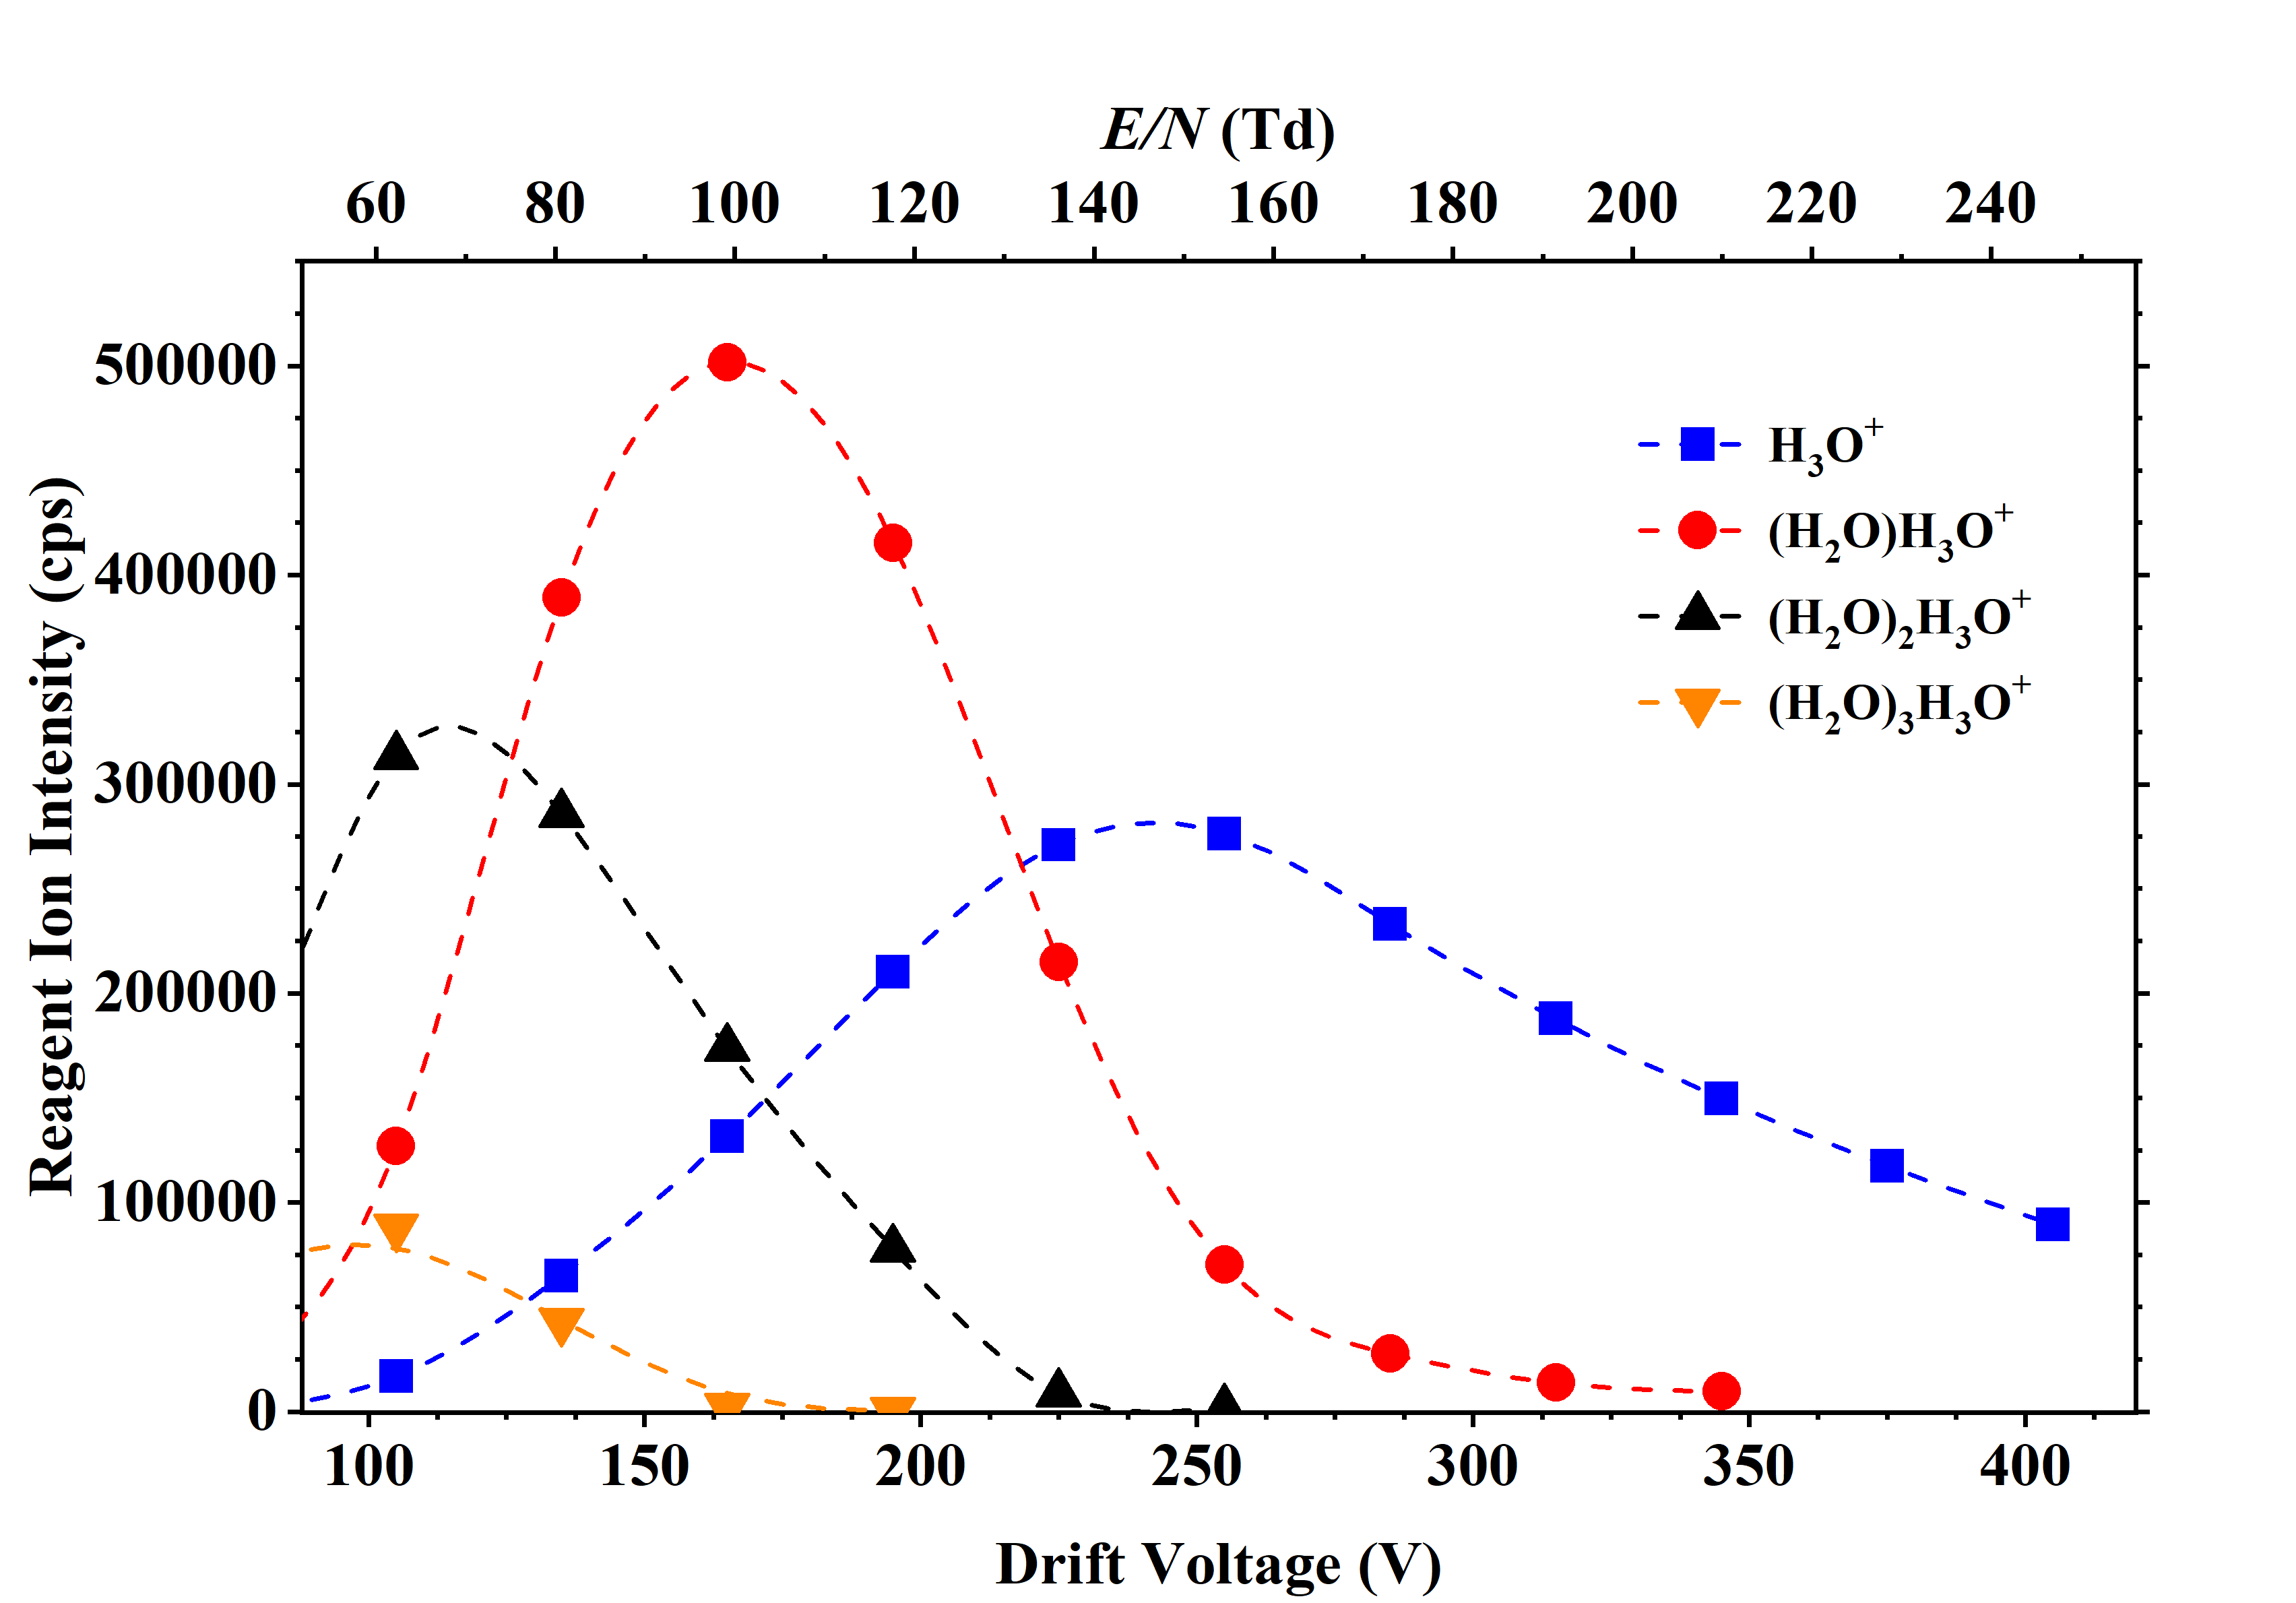
\includegraphics[width=0.6\linewidth]{pics/RInitros.png}\label{fig:ri1}}

%\sidesubfloat[]{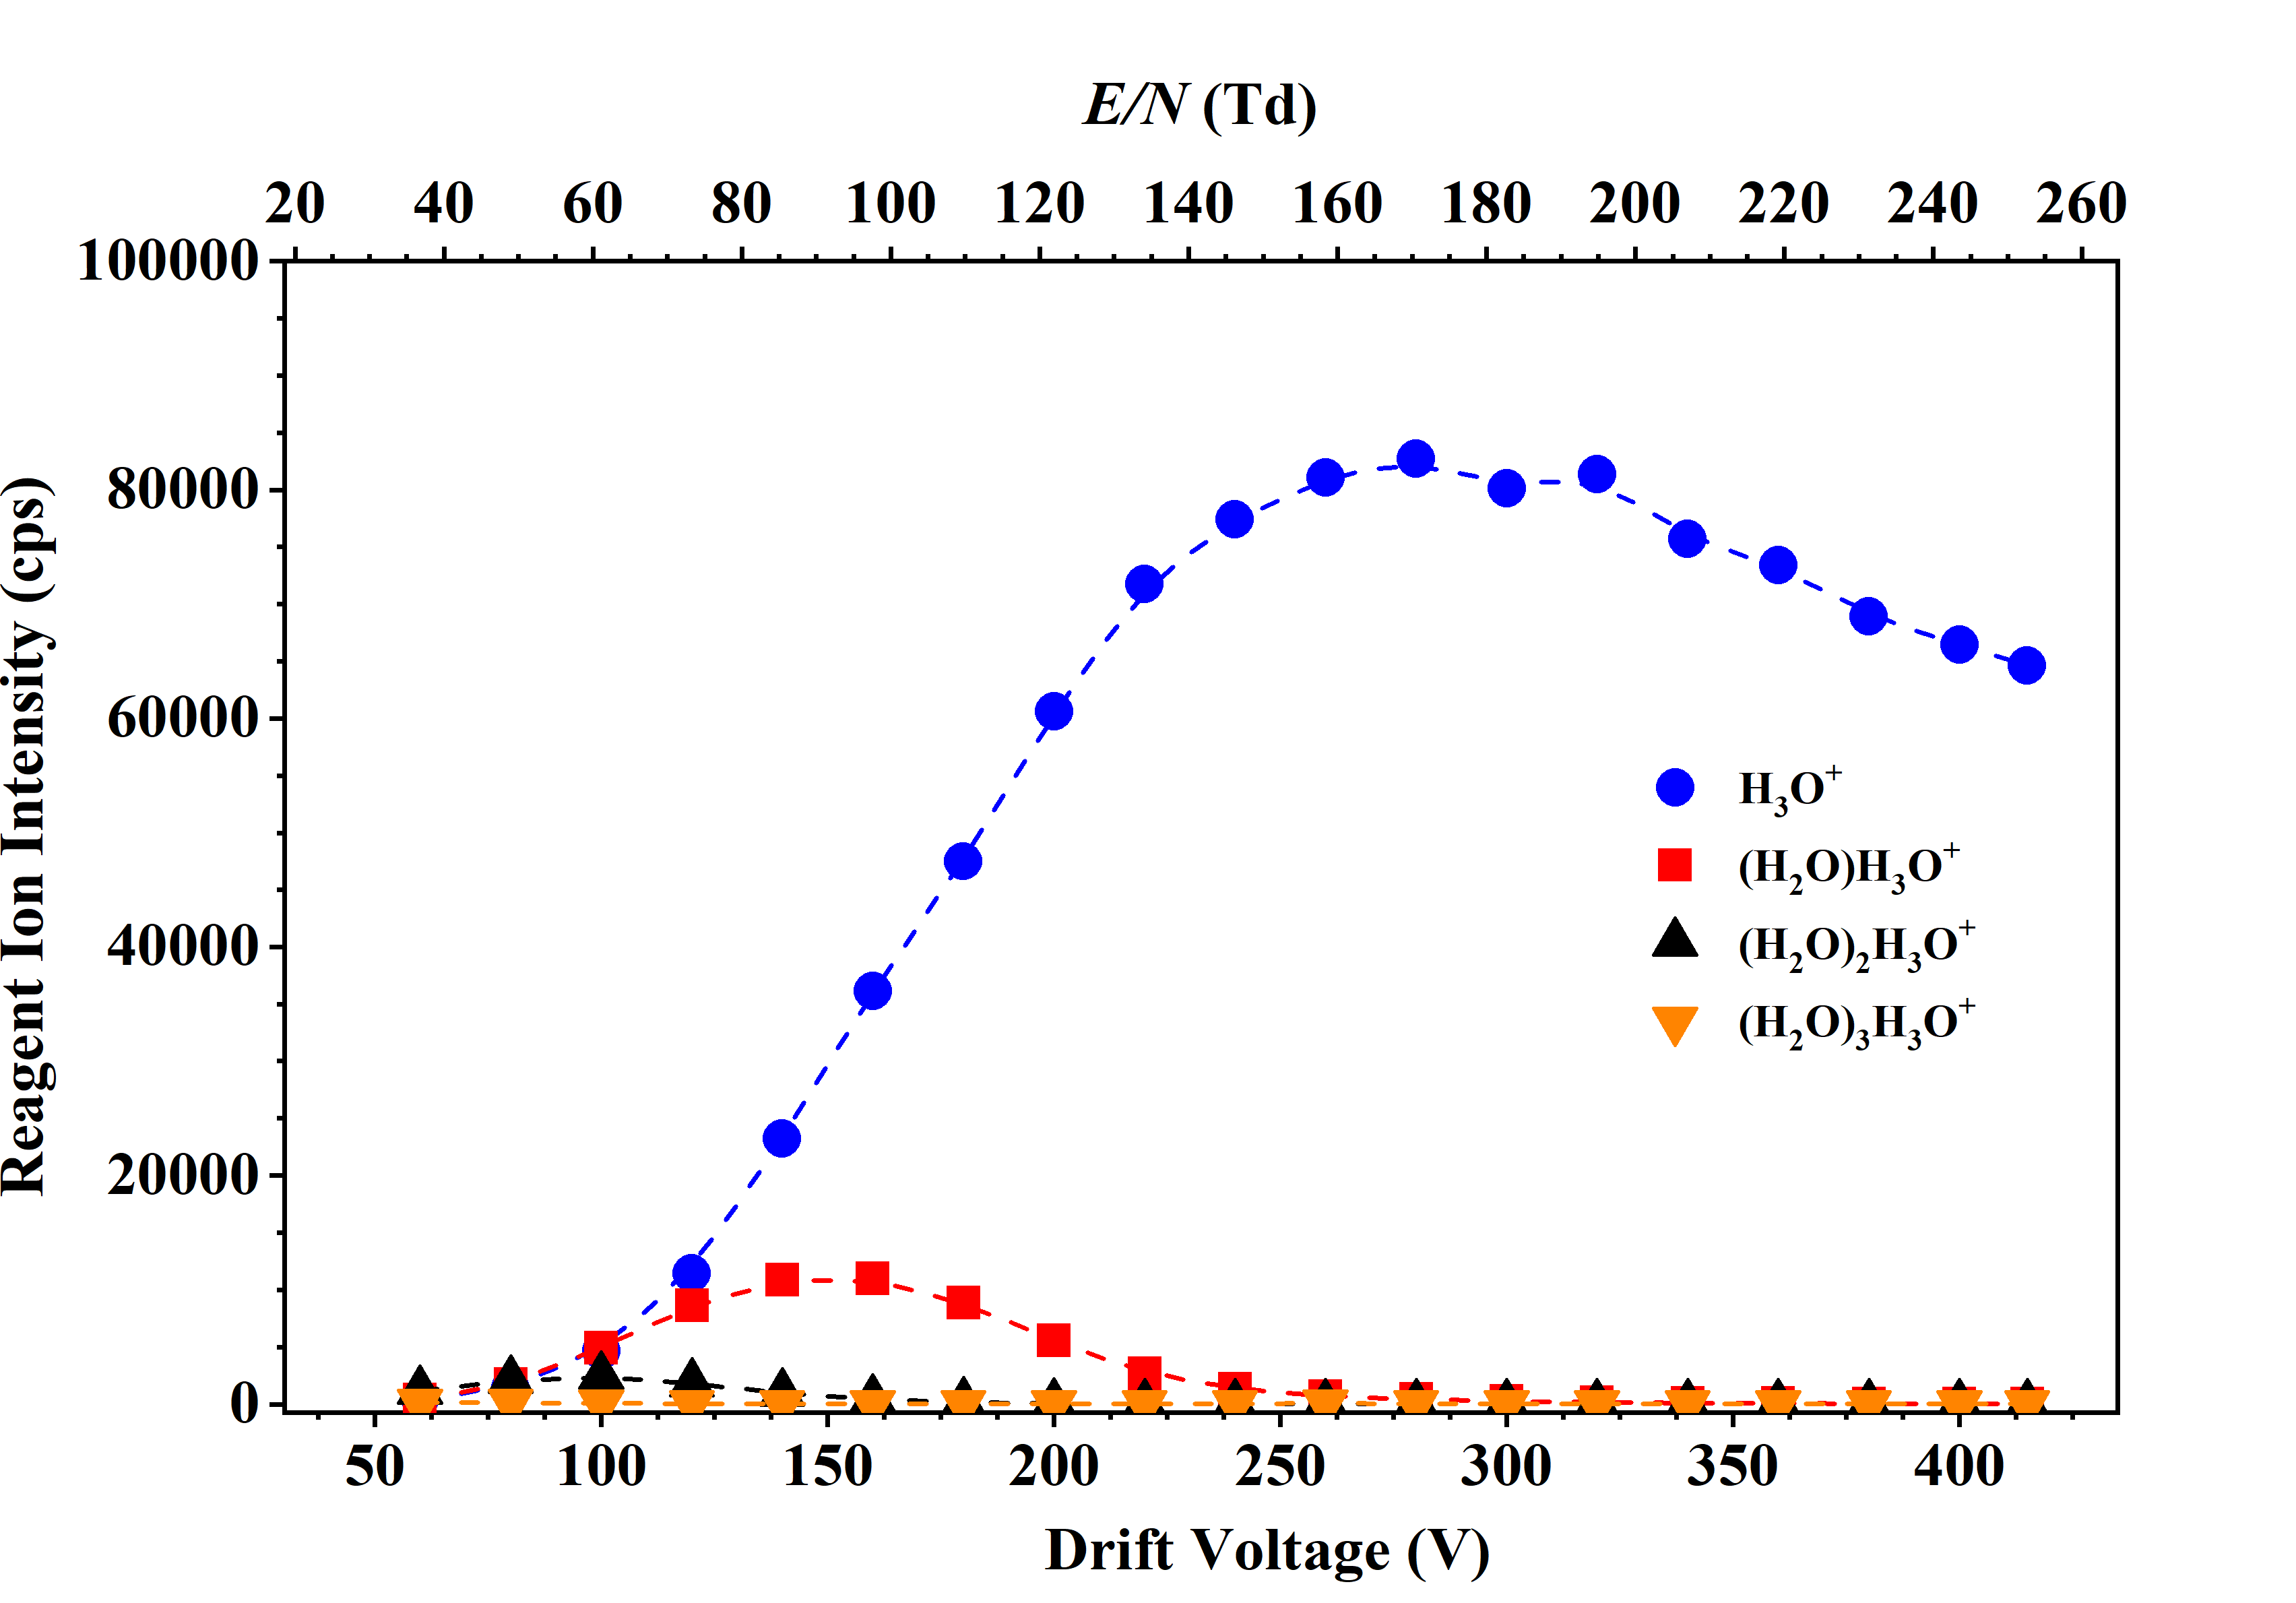
\includegraphics[width=0.6\linewidth]{pics/coc-RI.png}}

%\sidesubfloat[]{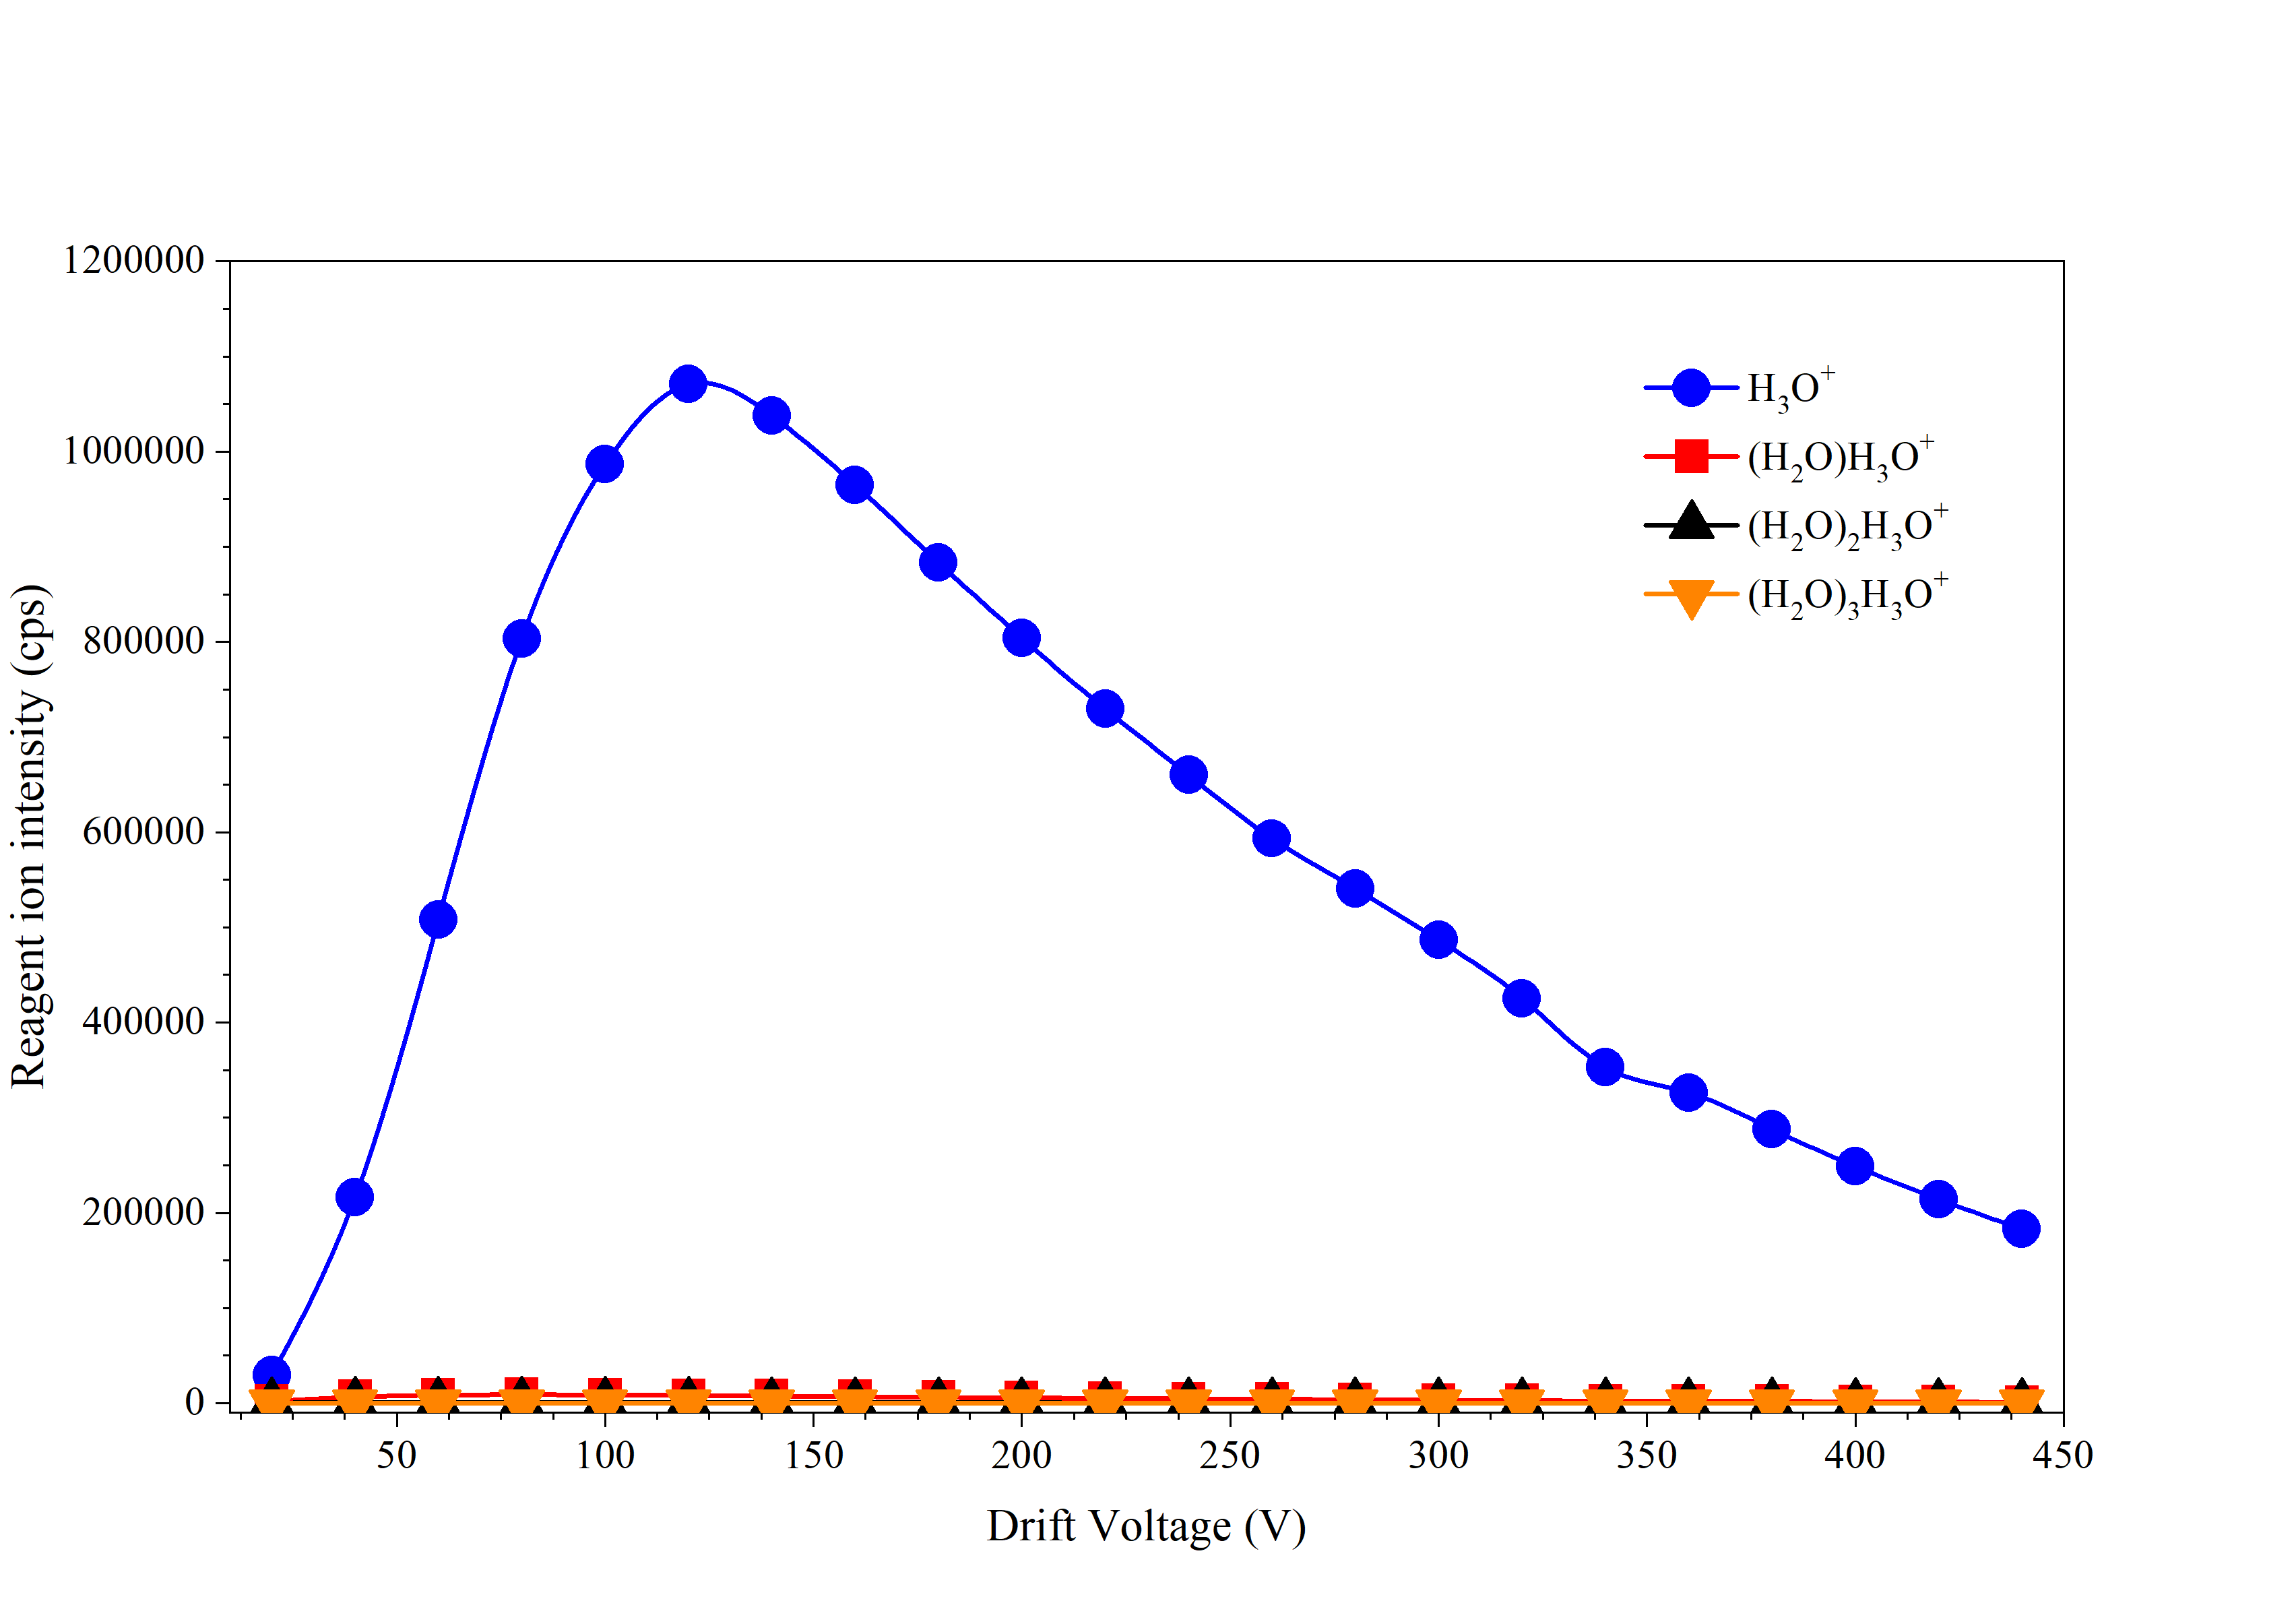
\includegraphics[width=0.6\linewidth]{pics/DPM_clusters_dry_RF.png}%water_RF.png}\label{fig:ri2}}
%\caption{Ion signal in counts per second (cps) for the reagent ions in (a) DC mode and (b) RF mode at 100$^{\circ}$C and 1 mbar. \textbf{Bottom one is from Lynx (MkII reactor)}}
%\label{fig:ri}
%\end{figure}













\subsection{Fast switching software}\label{sec:fs_data}
Analysing data from fast switching experiments can be tedious if needed to be done  manually file by file.
%
For this purpose, %and knowing already how to work with the experiment files, 
it was useful to write a script in Matlab\textsuperscript{\textregistered}  including  a graphical user interface to analyse the data in a quicker way.
%
This interface is shown in \autoref{fig:fss}.
It basically imports the suitable files, opens the cumulative mass spectrum to select the regions of interest, calculates and plots the ion intensities splitting the data in frames (i.e. each of the time intervals in which the drift tube is kept at the same \textit{E/N}), and exports the data to an excel file in both counts per second and branching ratios together with the experiment time and the \textit{E/N}.
%
Note that different colours are used in the raw and averaged data to ease the visualisation.

\begin{figure}%[t]
\centering
\sidesubfloat[]{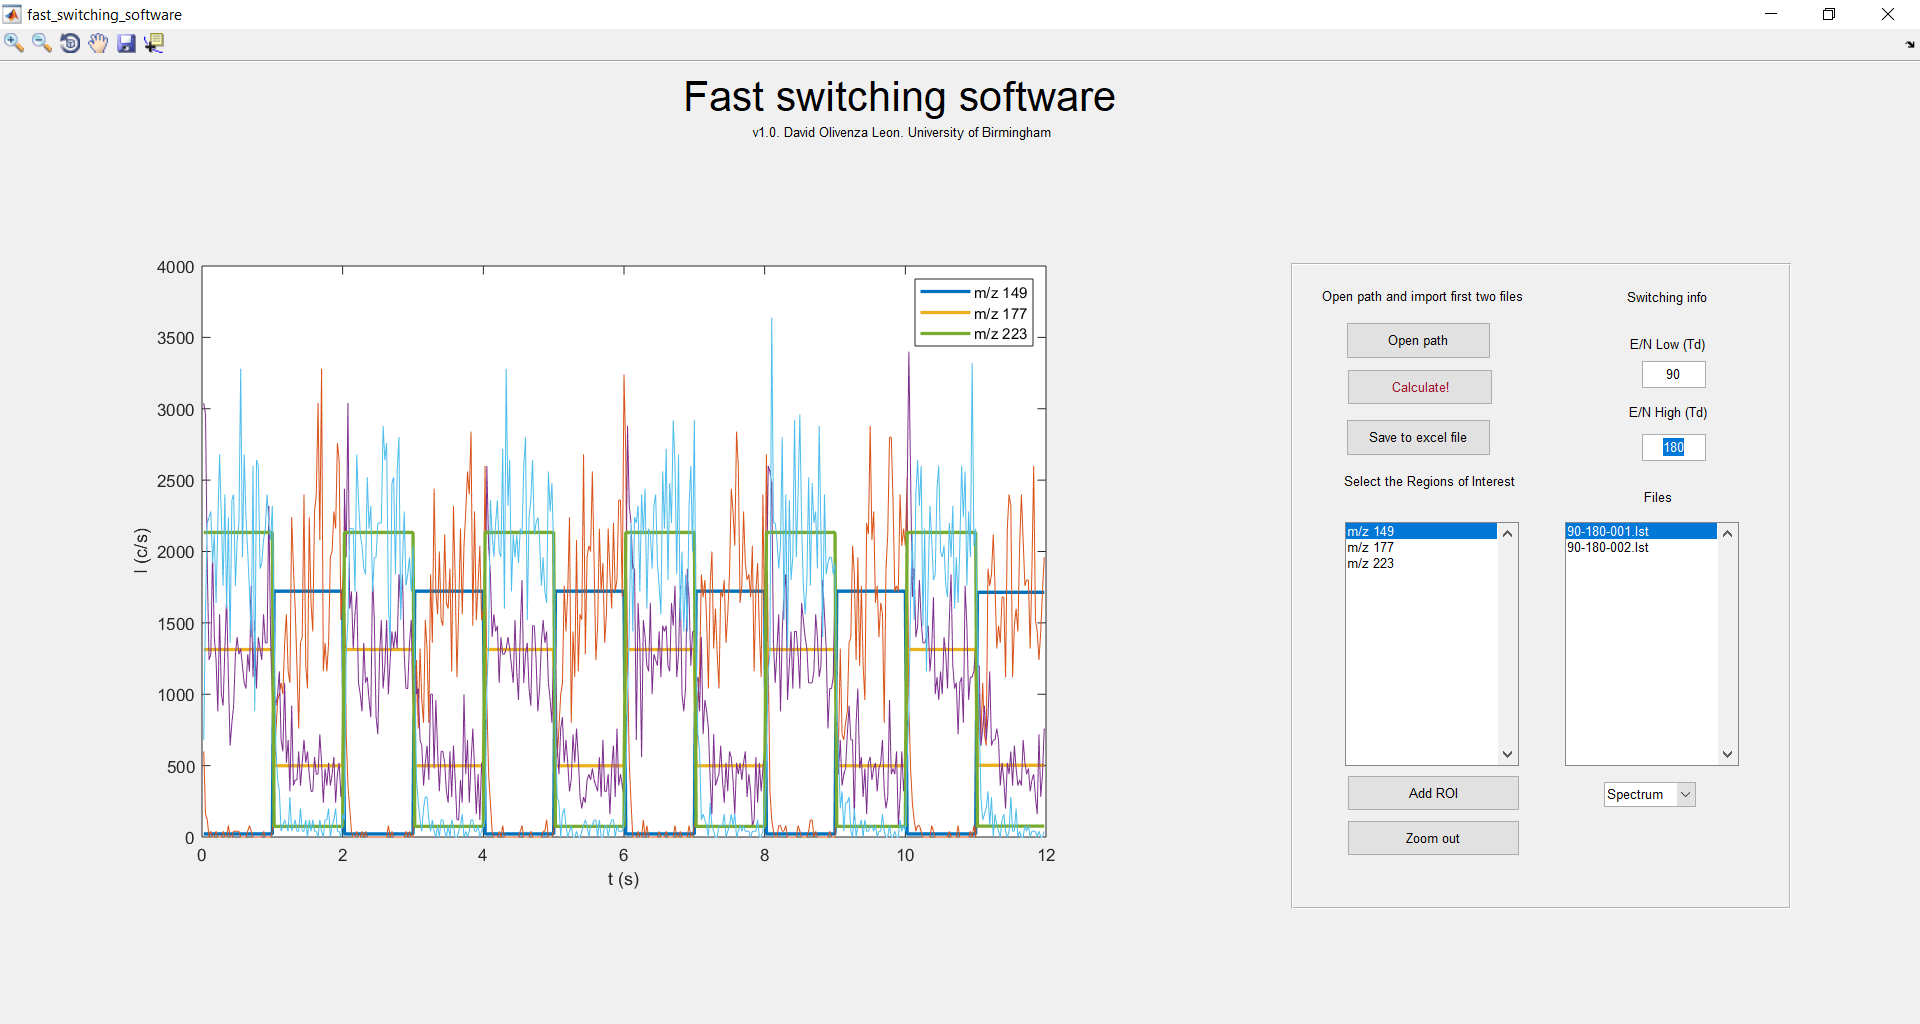
\includegraphics[width=0.9\linewidth]{pics/fss.png}}

\sidesubfloat[]{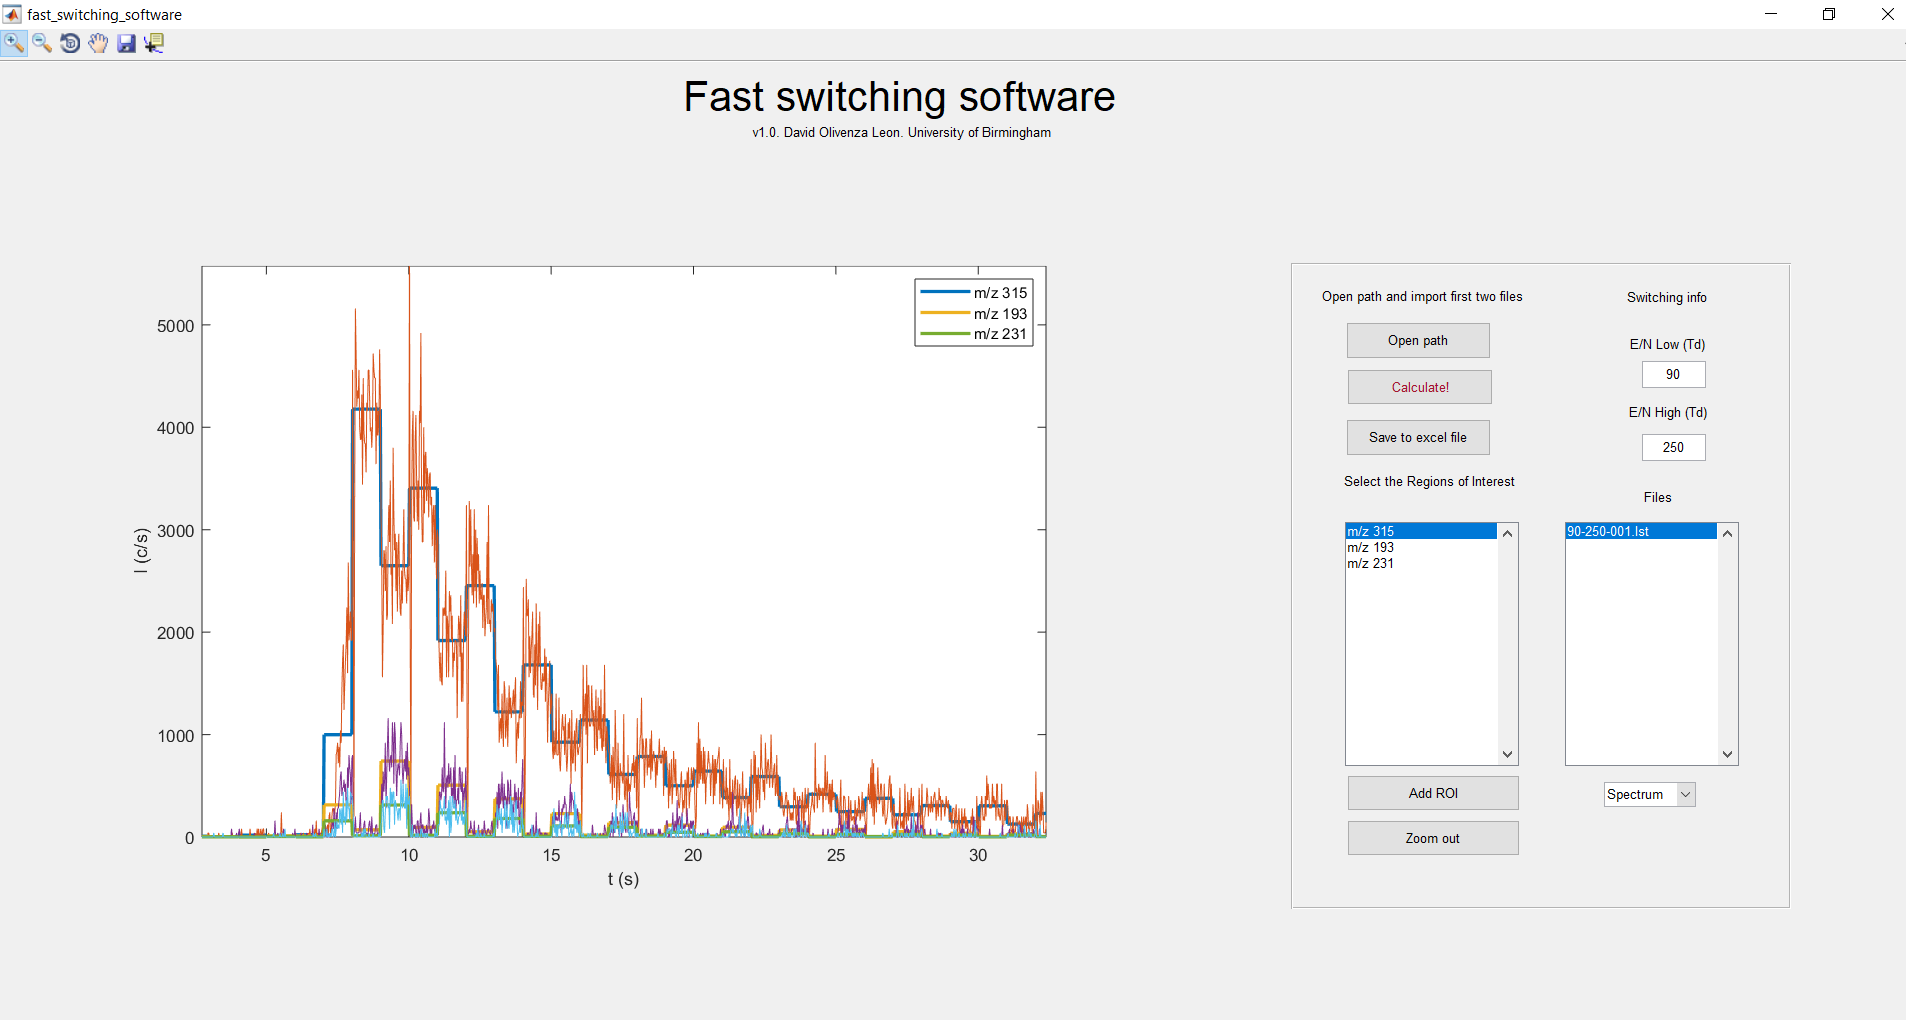
\includegraphics[width=0.9\linewidth]{pics/fs_CBD.png}}
%\sidesubfloat[]{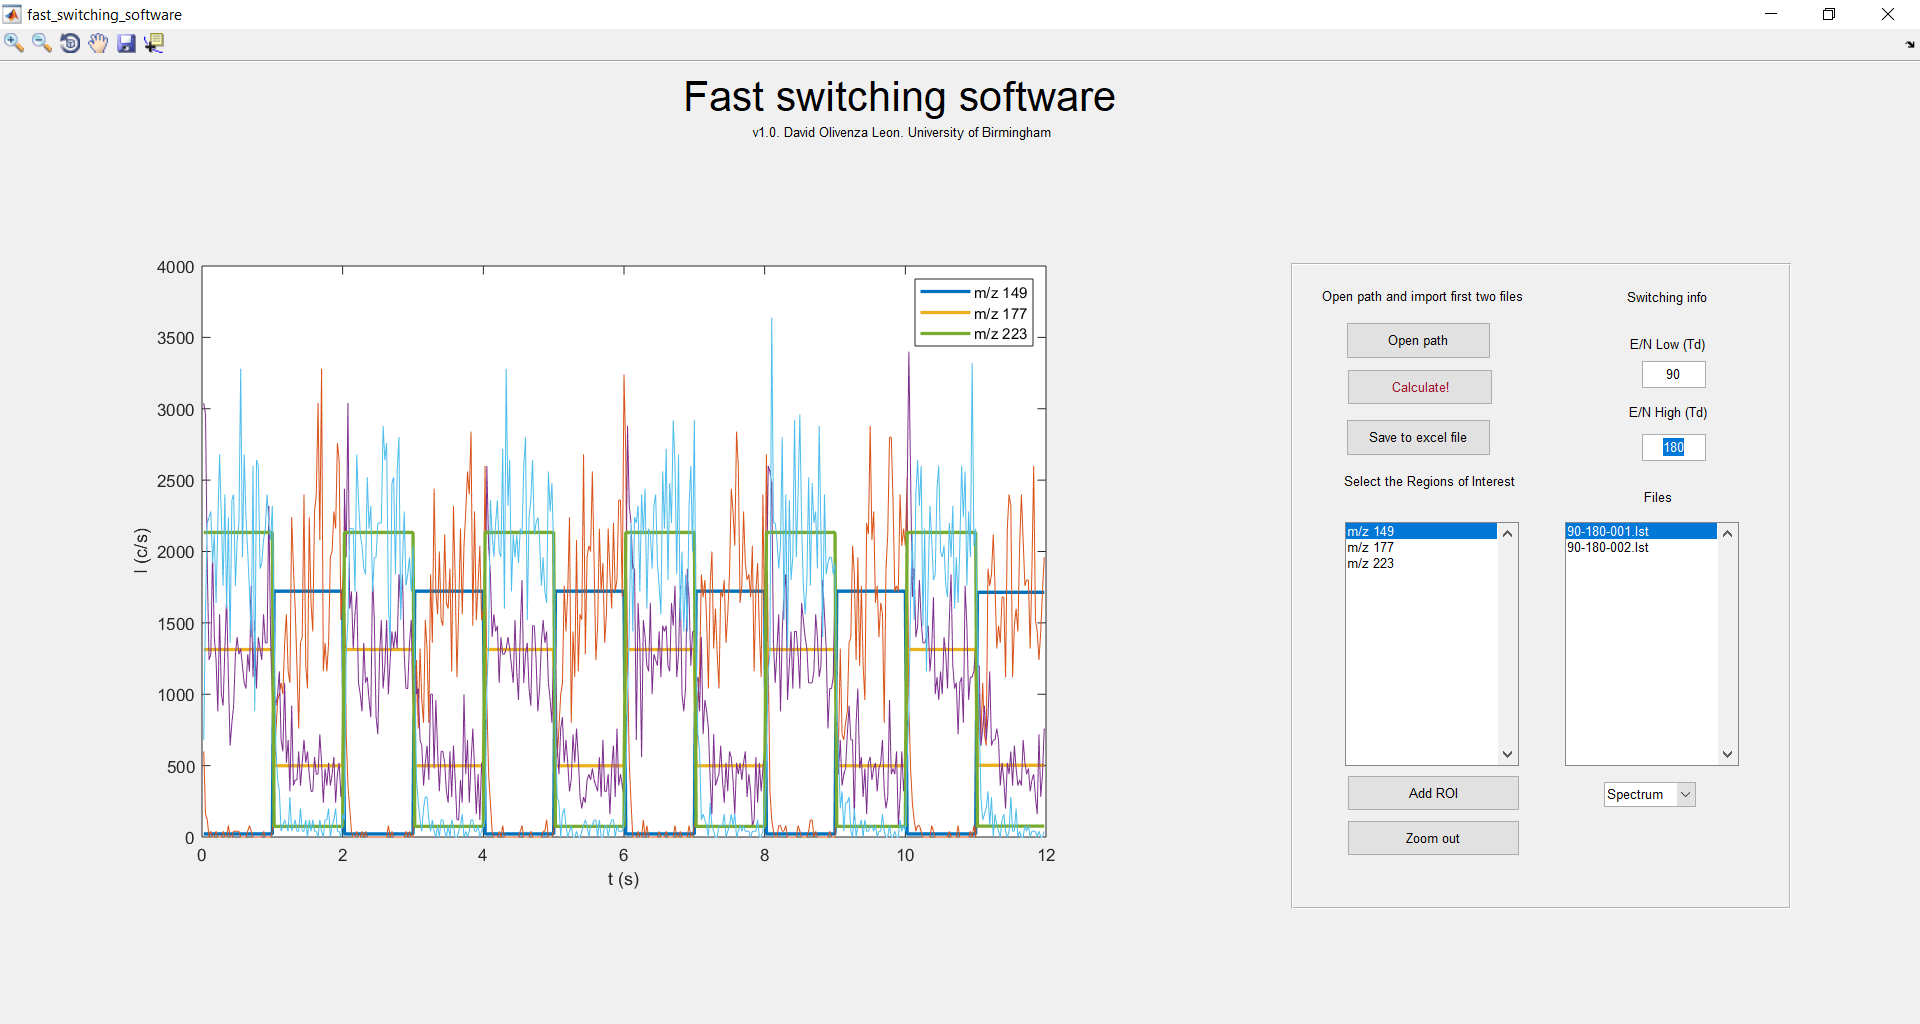
\includegraphics[height=0.4\textheight]{pics/fss.png}}
%\sidesubfloat[]{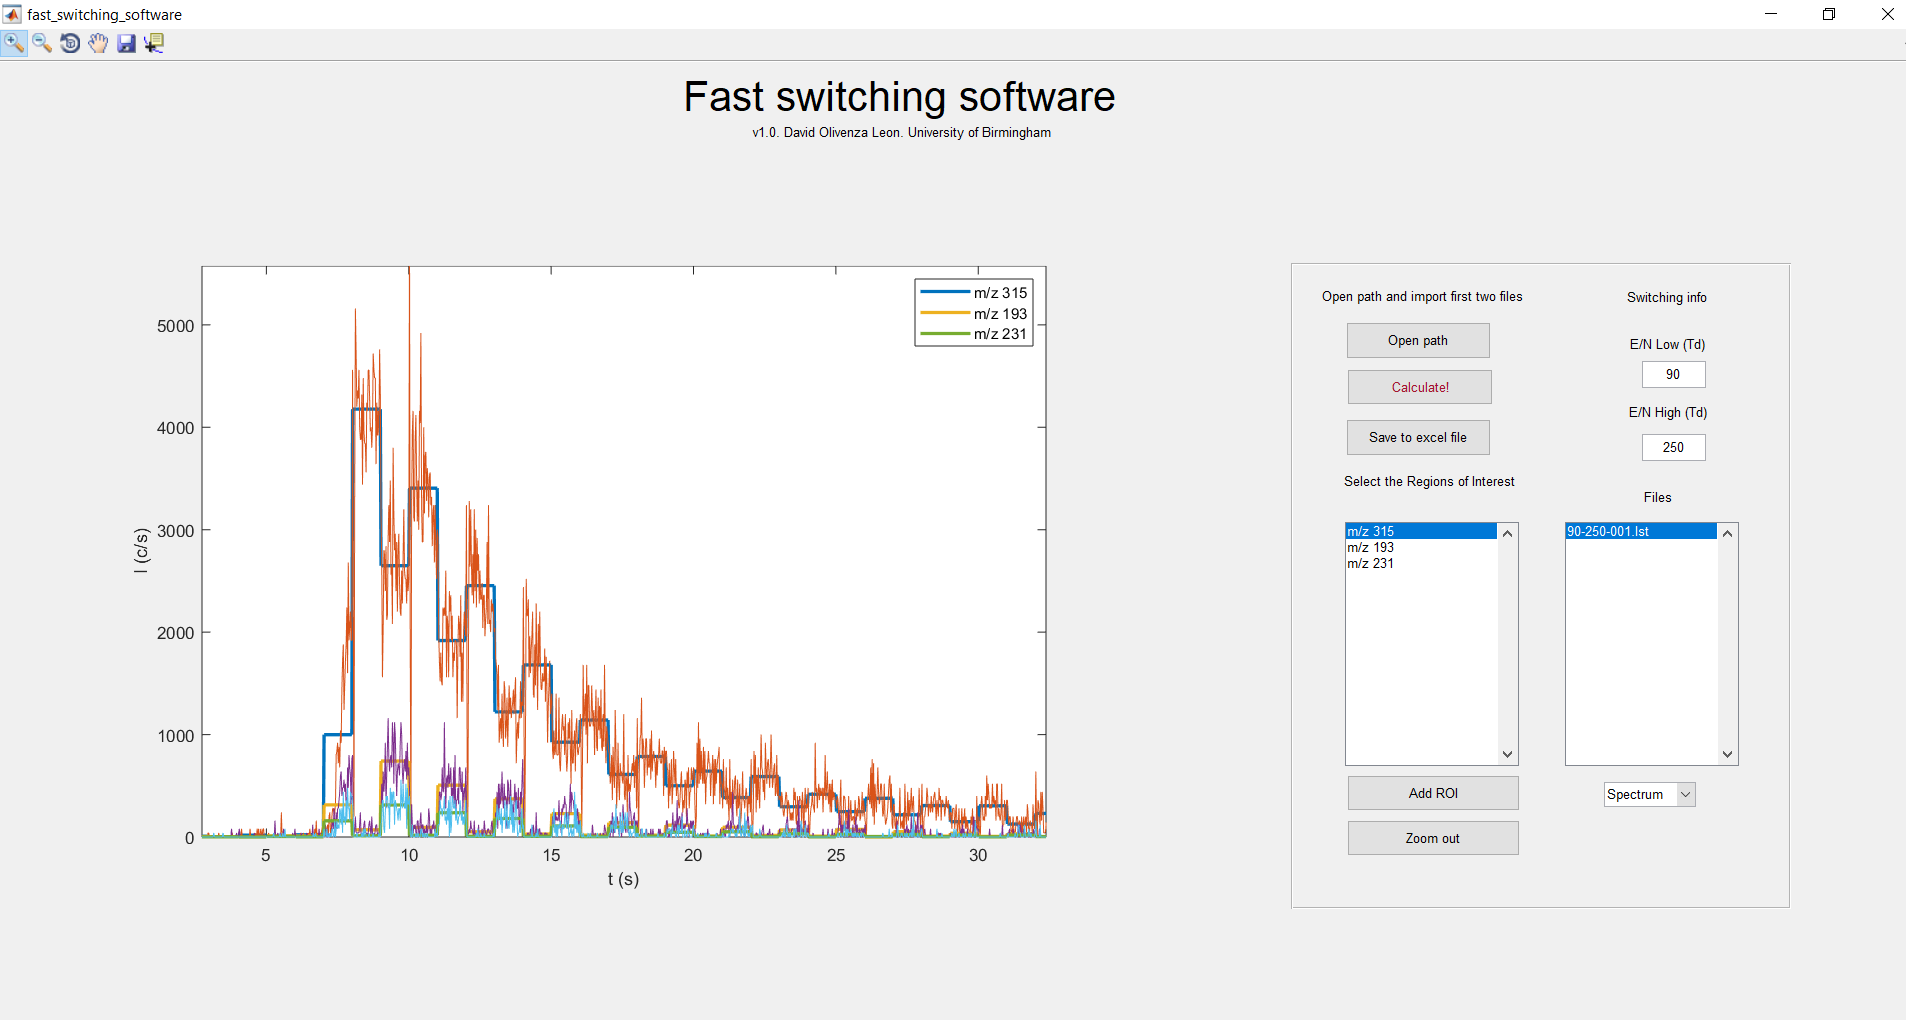
\includegraphics[height=0.4\textheight]{pics/fs_CBD.png}}
\caption[Screenshot of the graphical user interface for the script that  analyses  fast-switching data]{Screenshot of the graphical user interface for the script that  analyses  fast-switching data for: (a)  a steady signal, and (b) a transient experiment.}
\label{fig:fss}
\end{figure}

The files that this script imports are the .lst ones and their accompanying .ini files, which contain the information of the fast switching experiment that is necessary to work with the data.
This  comprehends, among other parameters,
the number of phases,
the number of cycles per phase,
the total number of cycles,
the cycle period,
the number of frames
and
the dead time of the switching.
The number of phases refers to the number of different values that the \textit{E/N} takes during a single experiment. This value is two for the fast switching experiments, which we will refer to as \textit{E/N} low  and \textit{E/N} high.
%
The fast switching frequency is not explicitly recorded but it is given by the inverse of multiplying the cycle period by the number of cycles per phase. For instance, for a cycle period of 40 µs and 25000 cycles per phase, the switching frequency is 1 Hz.
%
The total length of the experiment is not recorded either but, similarly to the switching frequency, it can be calculated by multiplying the cycle period by the total number of cycles. For example, a cycle period of 40 µs and 1.5$\times$10$^6$ total cycles corresponds to a 1 minute experiment.
%
%
%Each of the time intervals in which the drift tube is kept at the same \textit{E/N} is called a frame. 
In a measurement lasting 60 seconds at a fast switching frequency of 1 Hz there are 60 total frames and 30 frames per phase.
%
%
The dead time recorded in the .ini file in this case refers to that given by the delay in the electronics to supply the right voltage to the drift tube (i.e. the rise and fall times) and it is around 70 ms. The software automatically ignores the interval three times bigger than this dead time to account for the capacitance of the reactor, which was explained  in section \ref{section:fs}.
%Phases = 2
%Frames = 30
%Cycle period us=40
%Number of cycles=1500000
%Phases=2
%Cycles per phase=25000
%Frames=30
%Dead time ms=70




If the files are saved with the name format [\textit{low E/N}]-[\textit{high E/N}]-[\textit{file number}], the script automatically reads and writes in the output file the values of the low and high \textit{E/N}. If not, they must be manually added.
%
The data inside each frame can be exported in raw format or averaged.
For steady experiments like the one shown in \autoref{fig:fss}a, the data from all the frames from a phase (i.e. high or low \textit{E/N}) can also be averaged like it is shown in this figure. Obviously, this does not make sense for transient measurements like that in \autoref{fig:fss}b.
%
Once the data analysis is finished, the results can be exported. The format these files are saved at allows easy double-y axis plot of the ion intensities and \textit{E/N} as a function of the experiment time, as it is shown in \autoref{fig:fss_plots}, for a (a,c) steady-state  and (b,d) transient measurement.




\begin{figure}[t]
\centering
\sidesubfloat[]{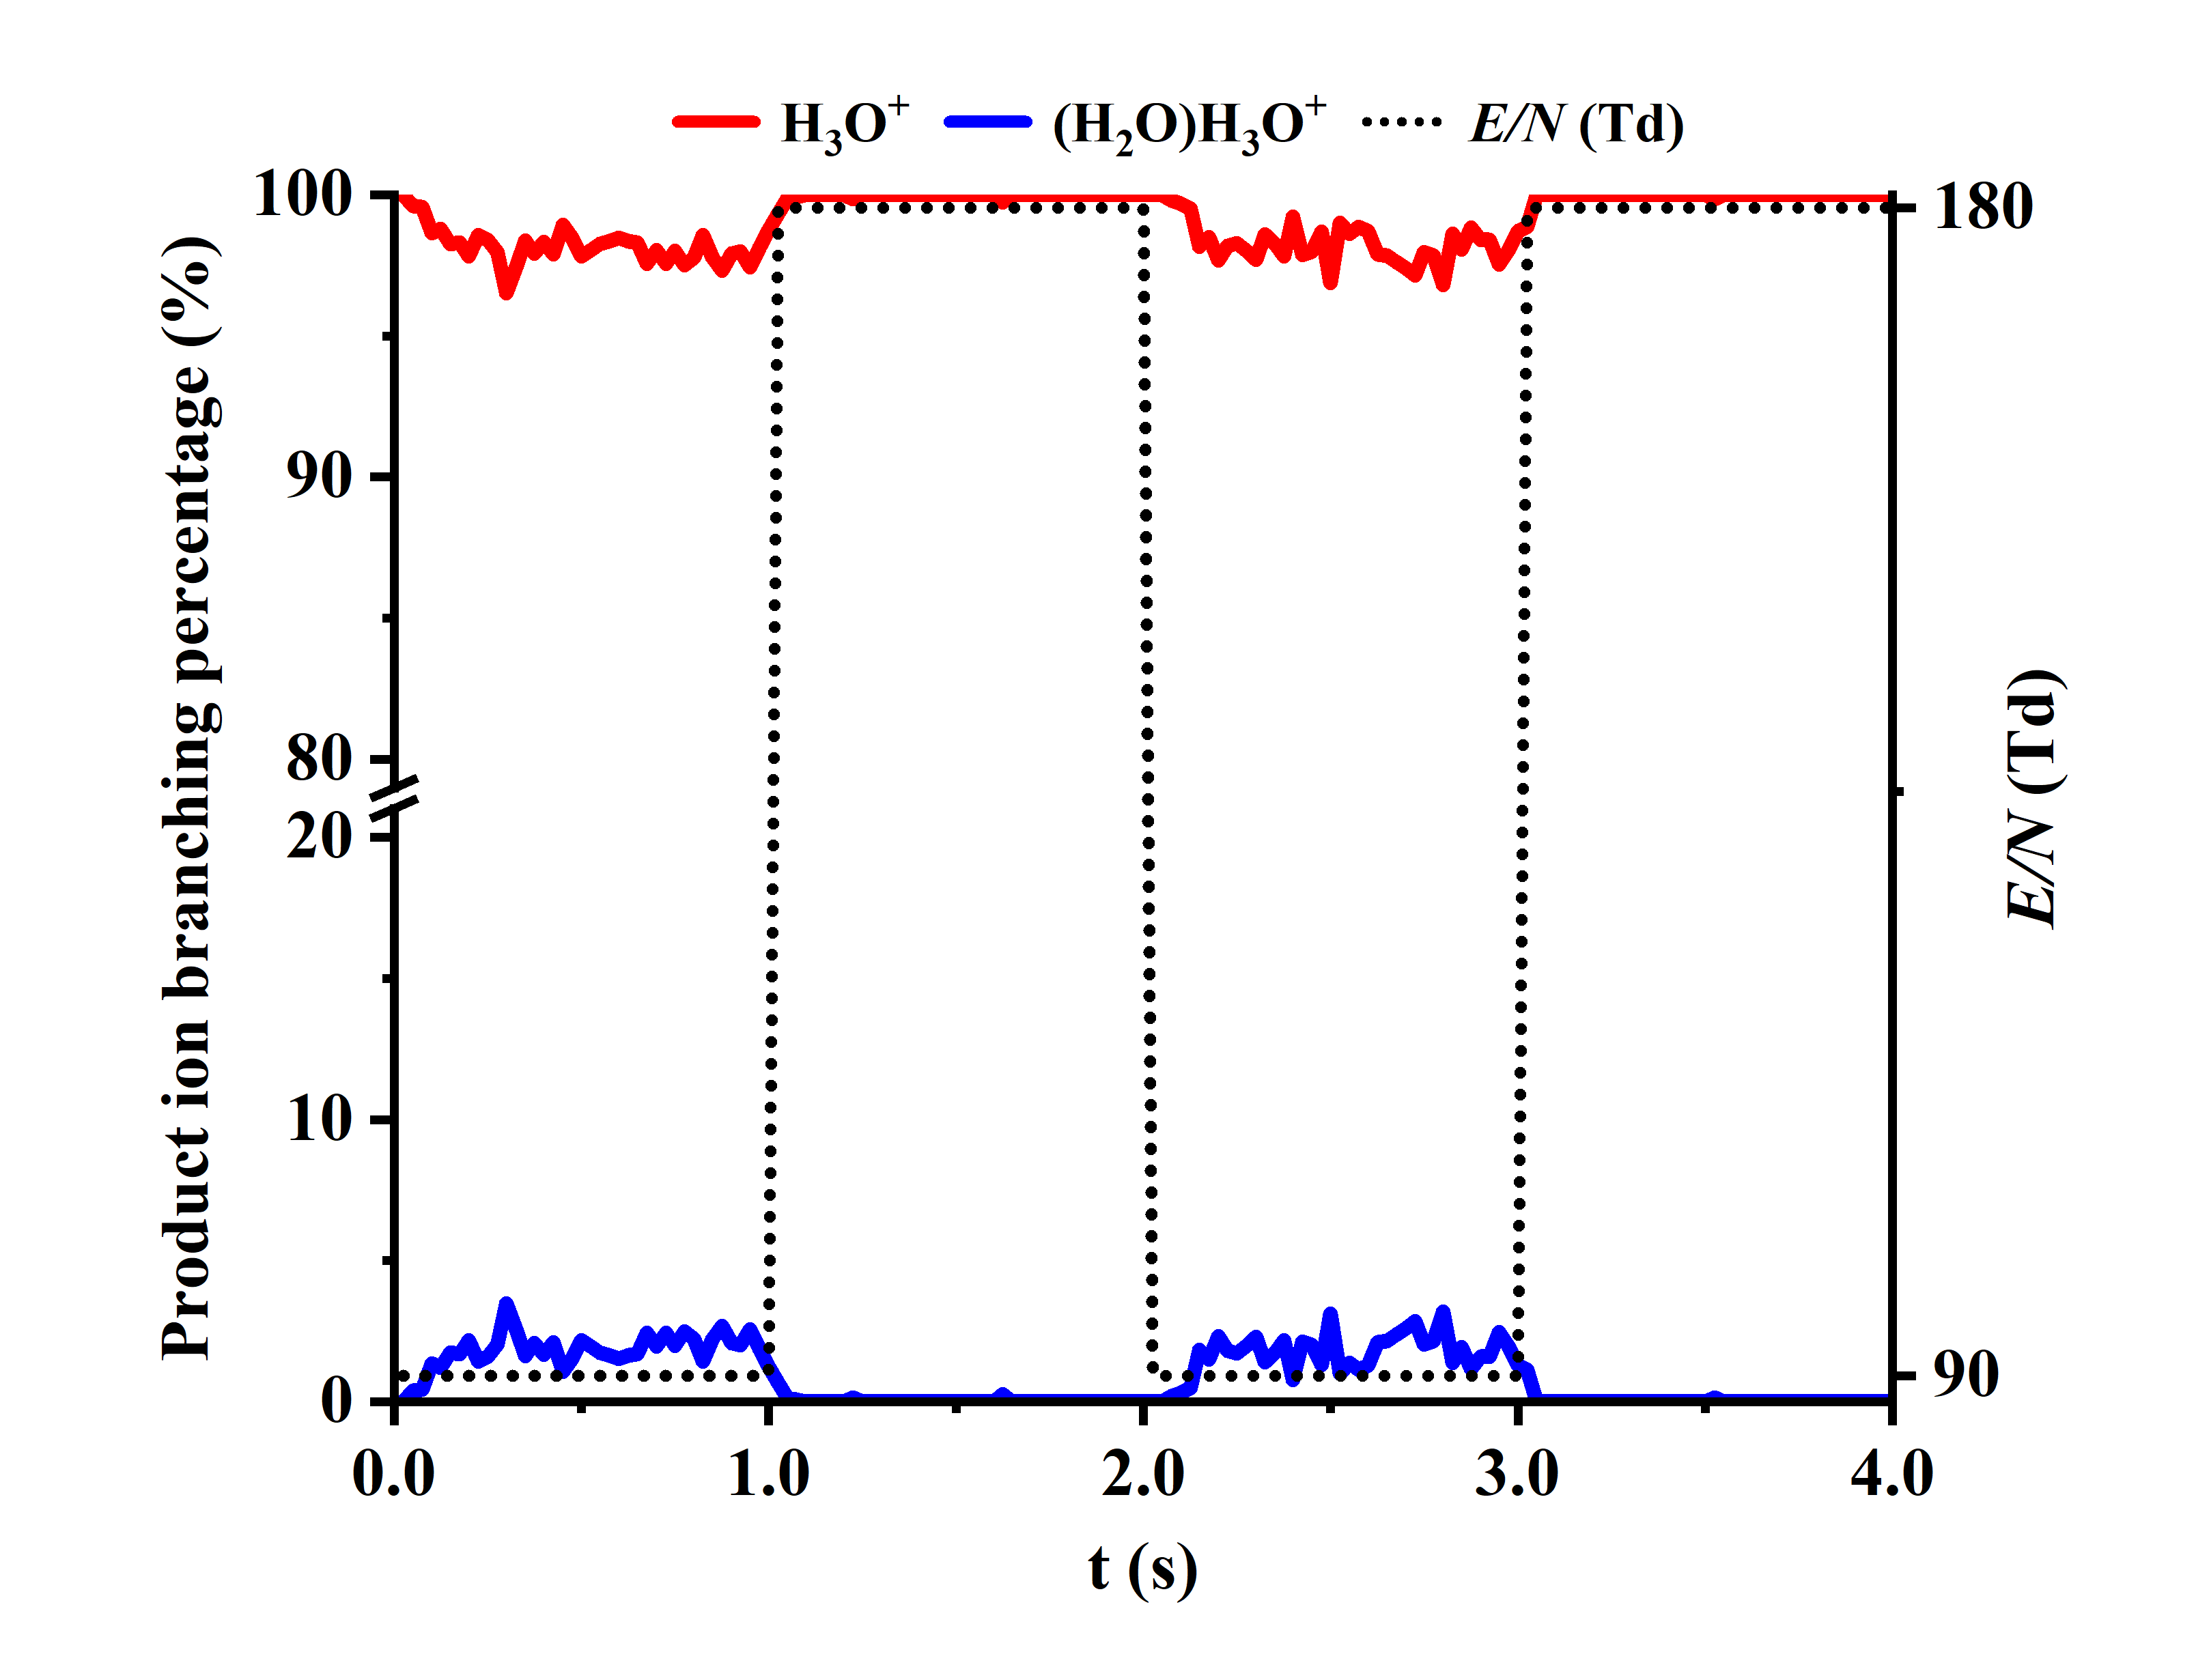
\includegraphics[width=0.45\textwidth]{pics/RIDPM90180Td.png}}
\sidesubfloat[]{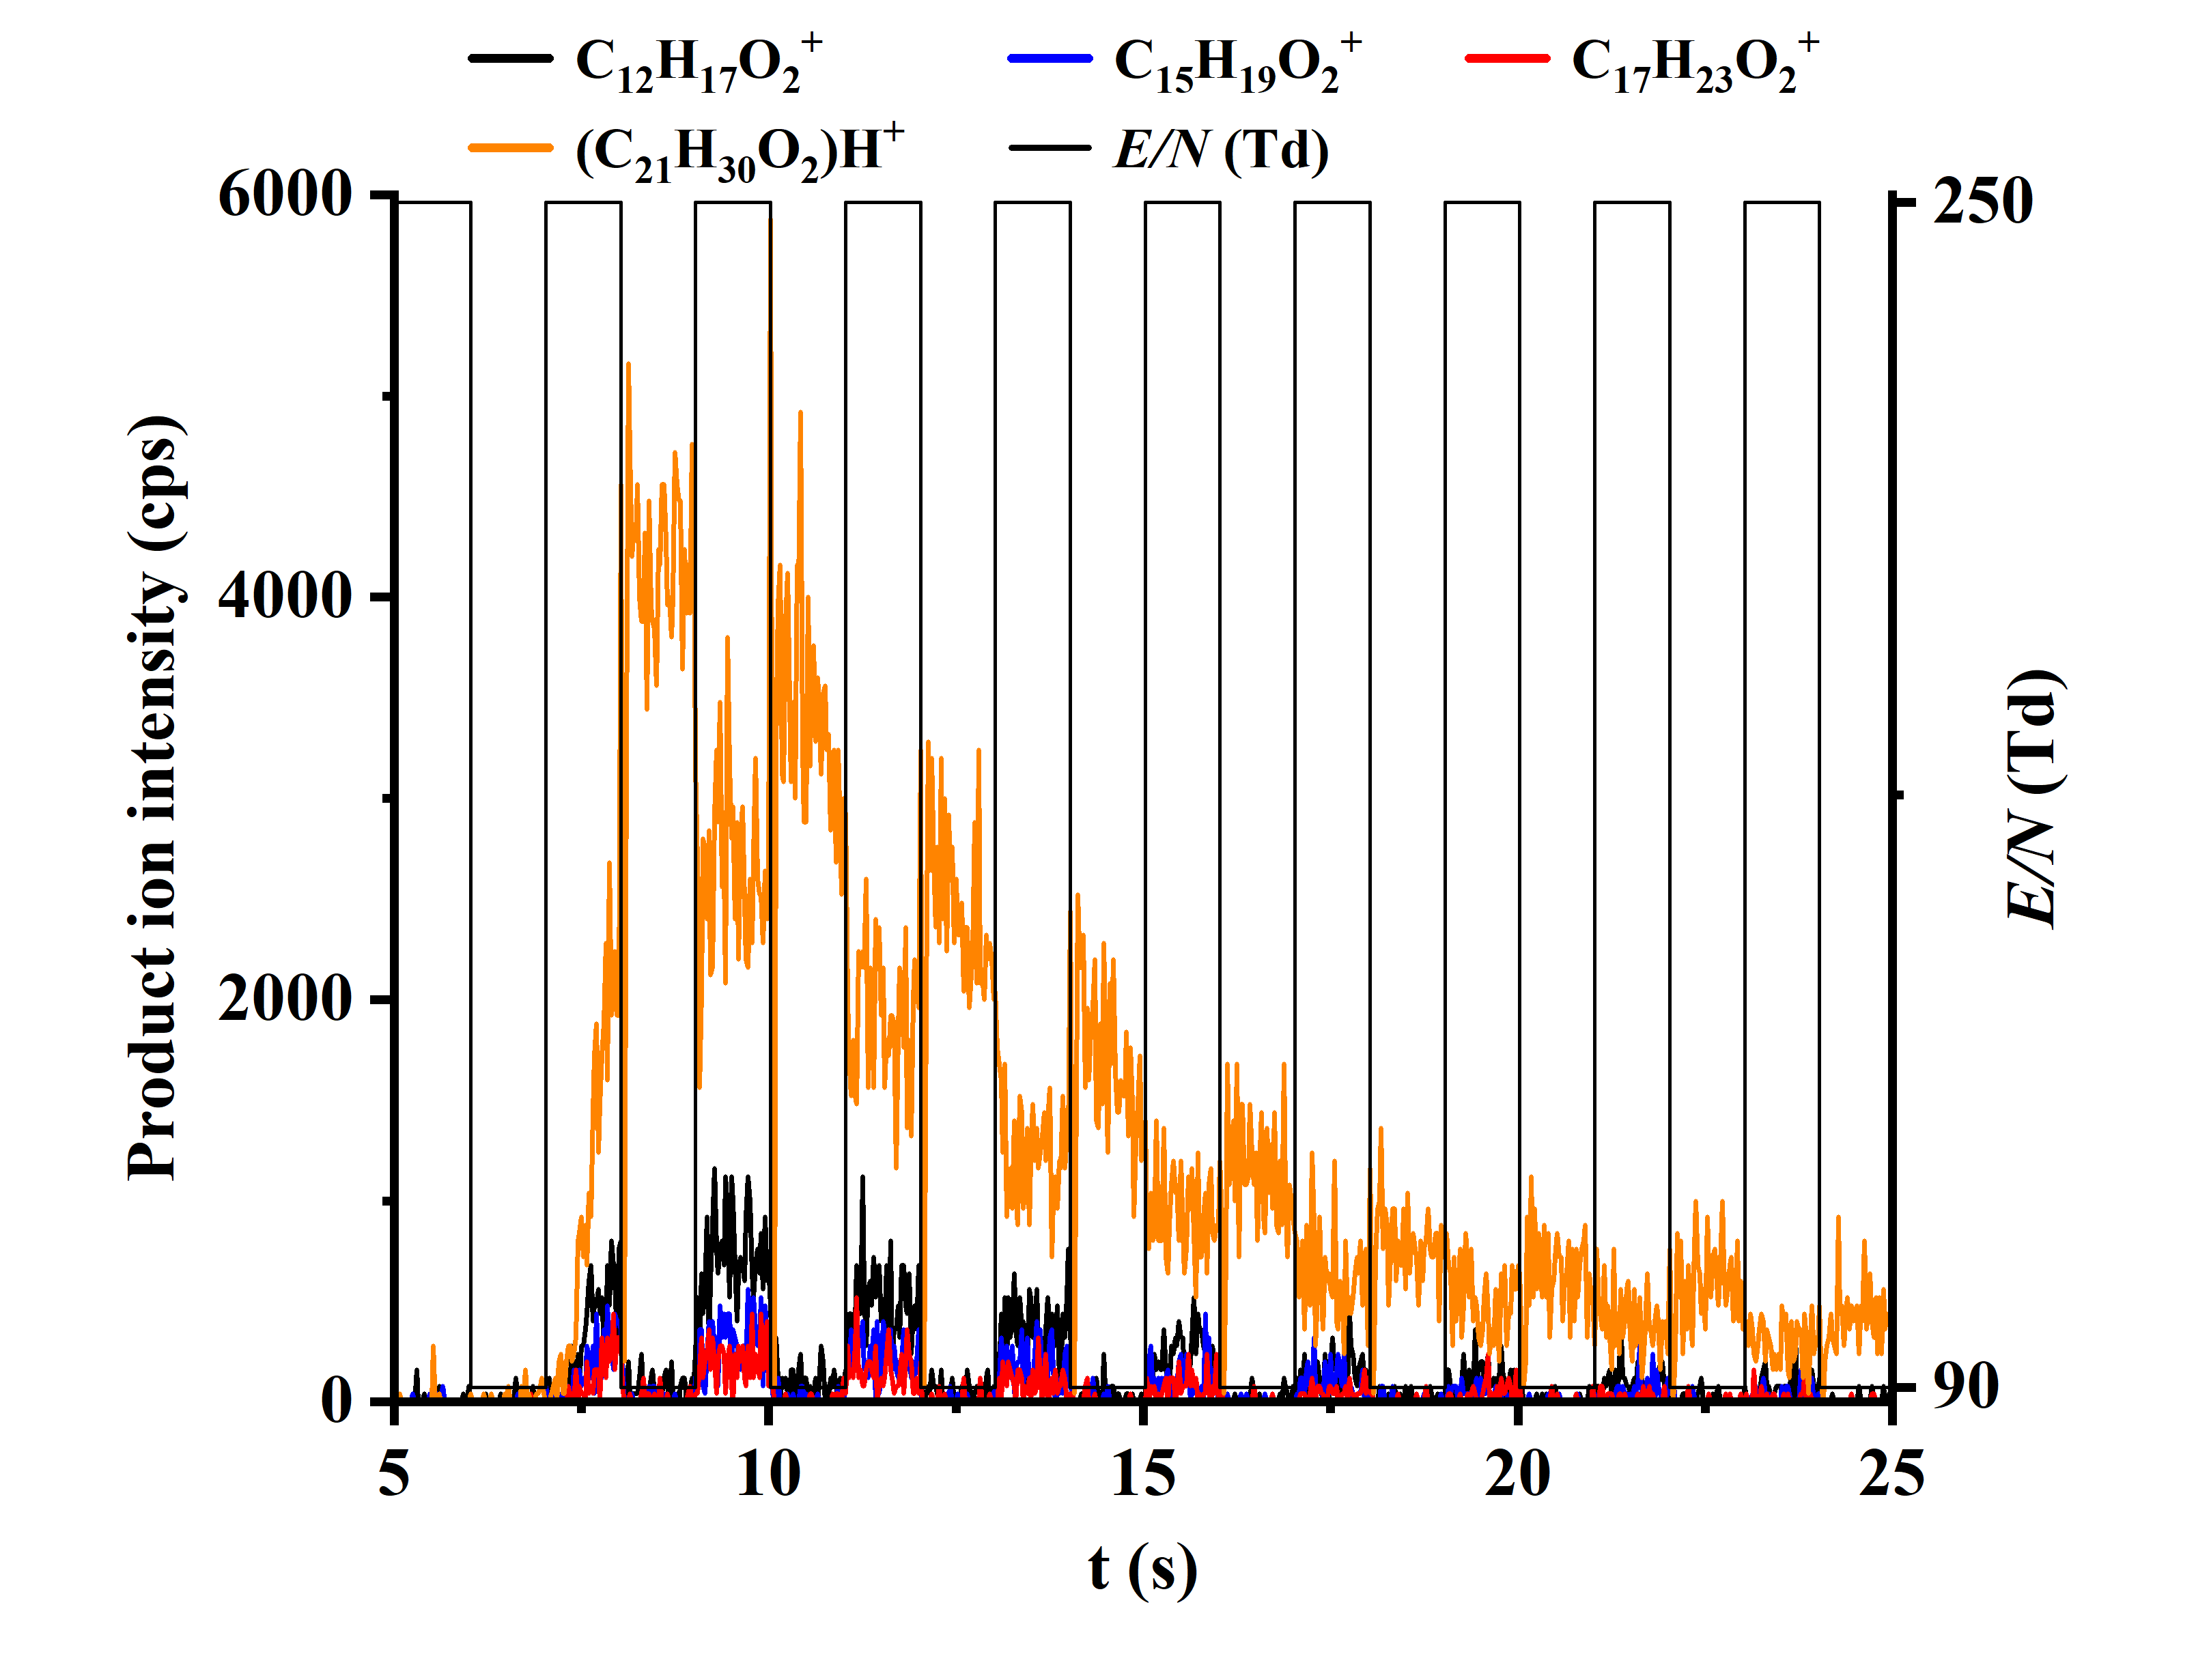
\includegraphics[width=0.45\textwidth]{pics/CBD-raw.png}}

\sidesubfloat[]{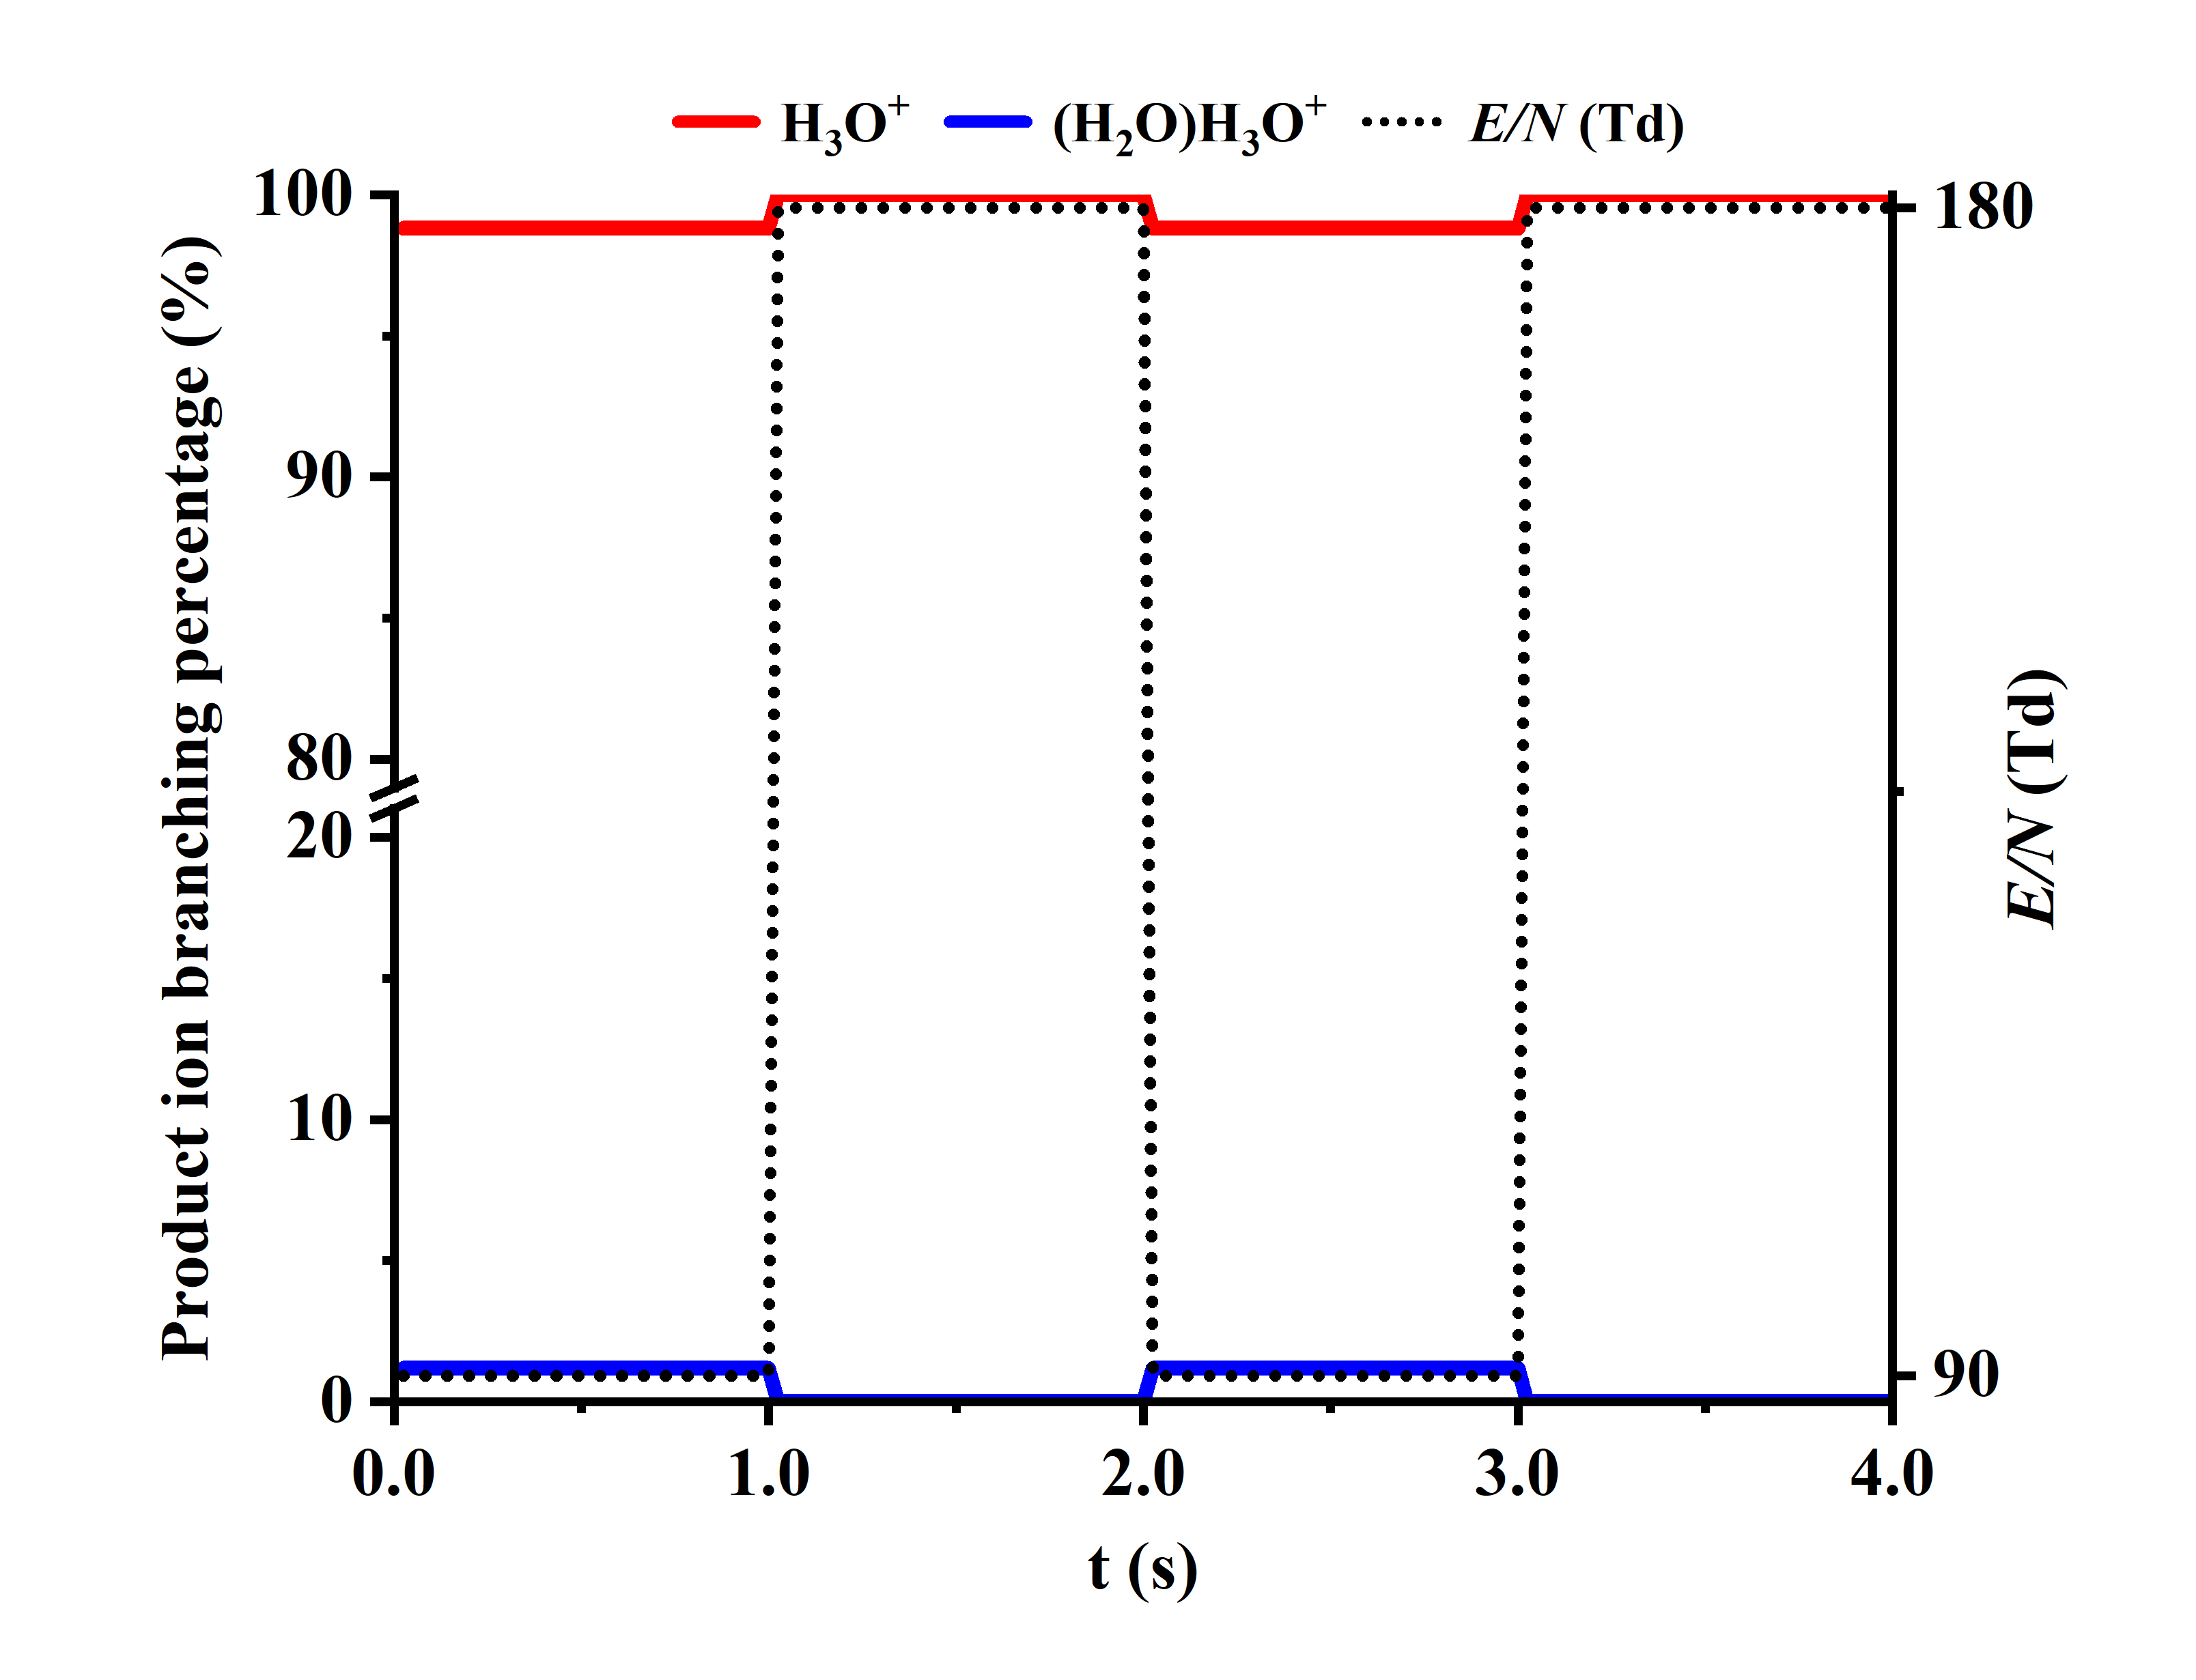
\includegraphics[width=0.45\textwidth]{pics/RIDPM90180Td-averaged.png}}
\sidesubfloat[]{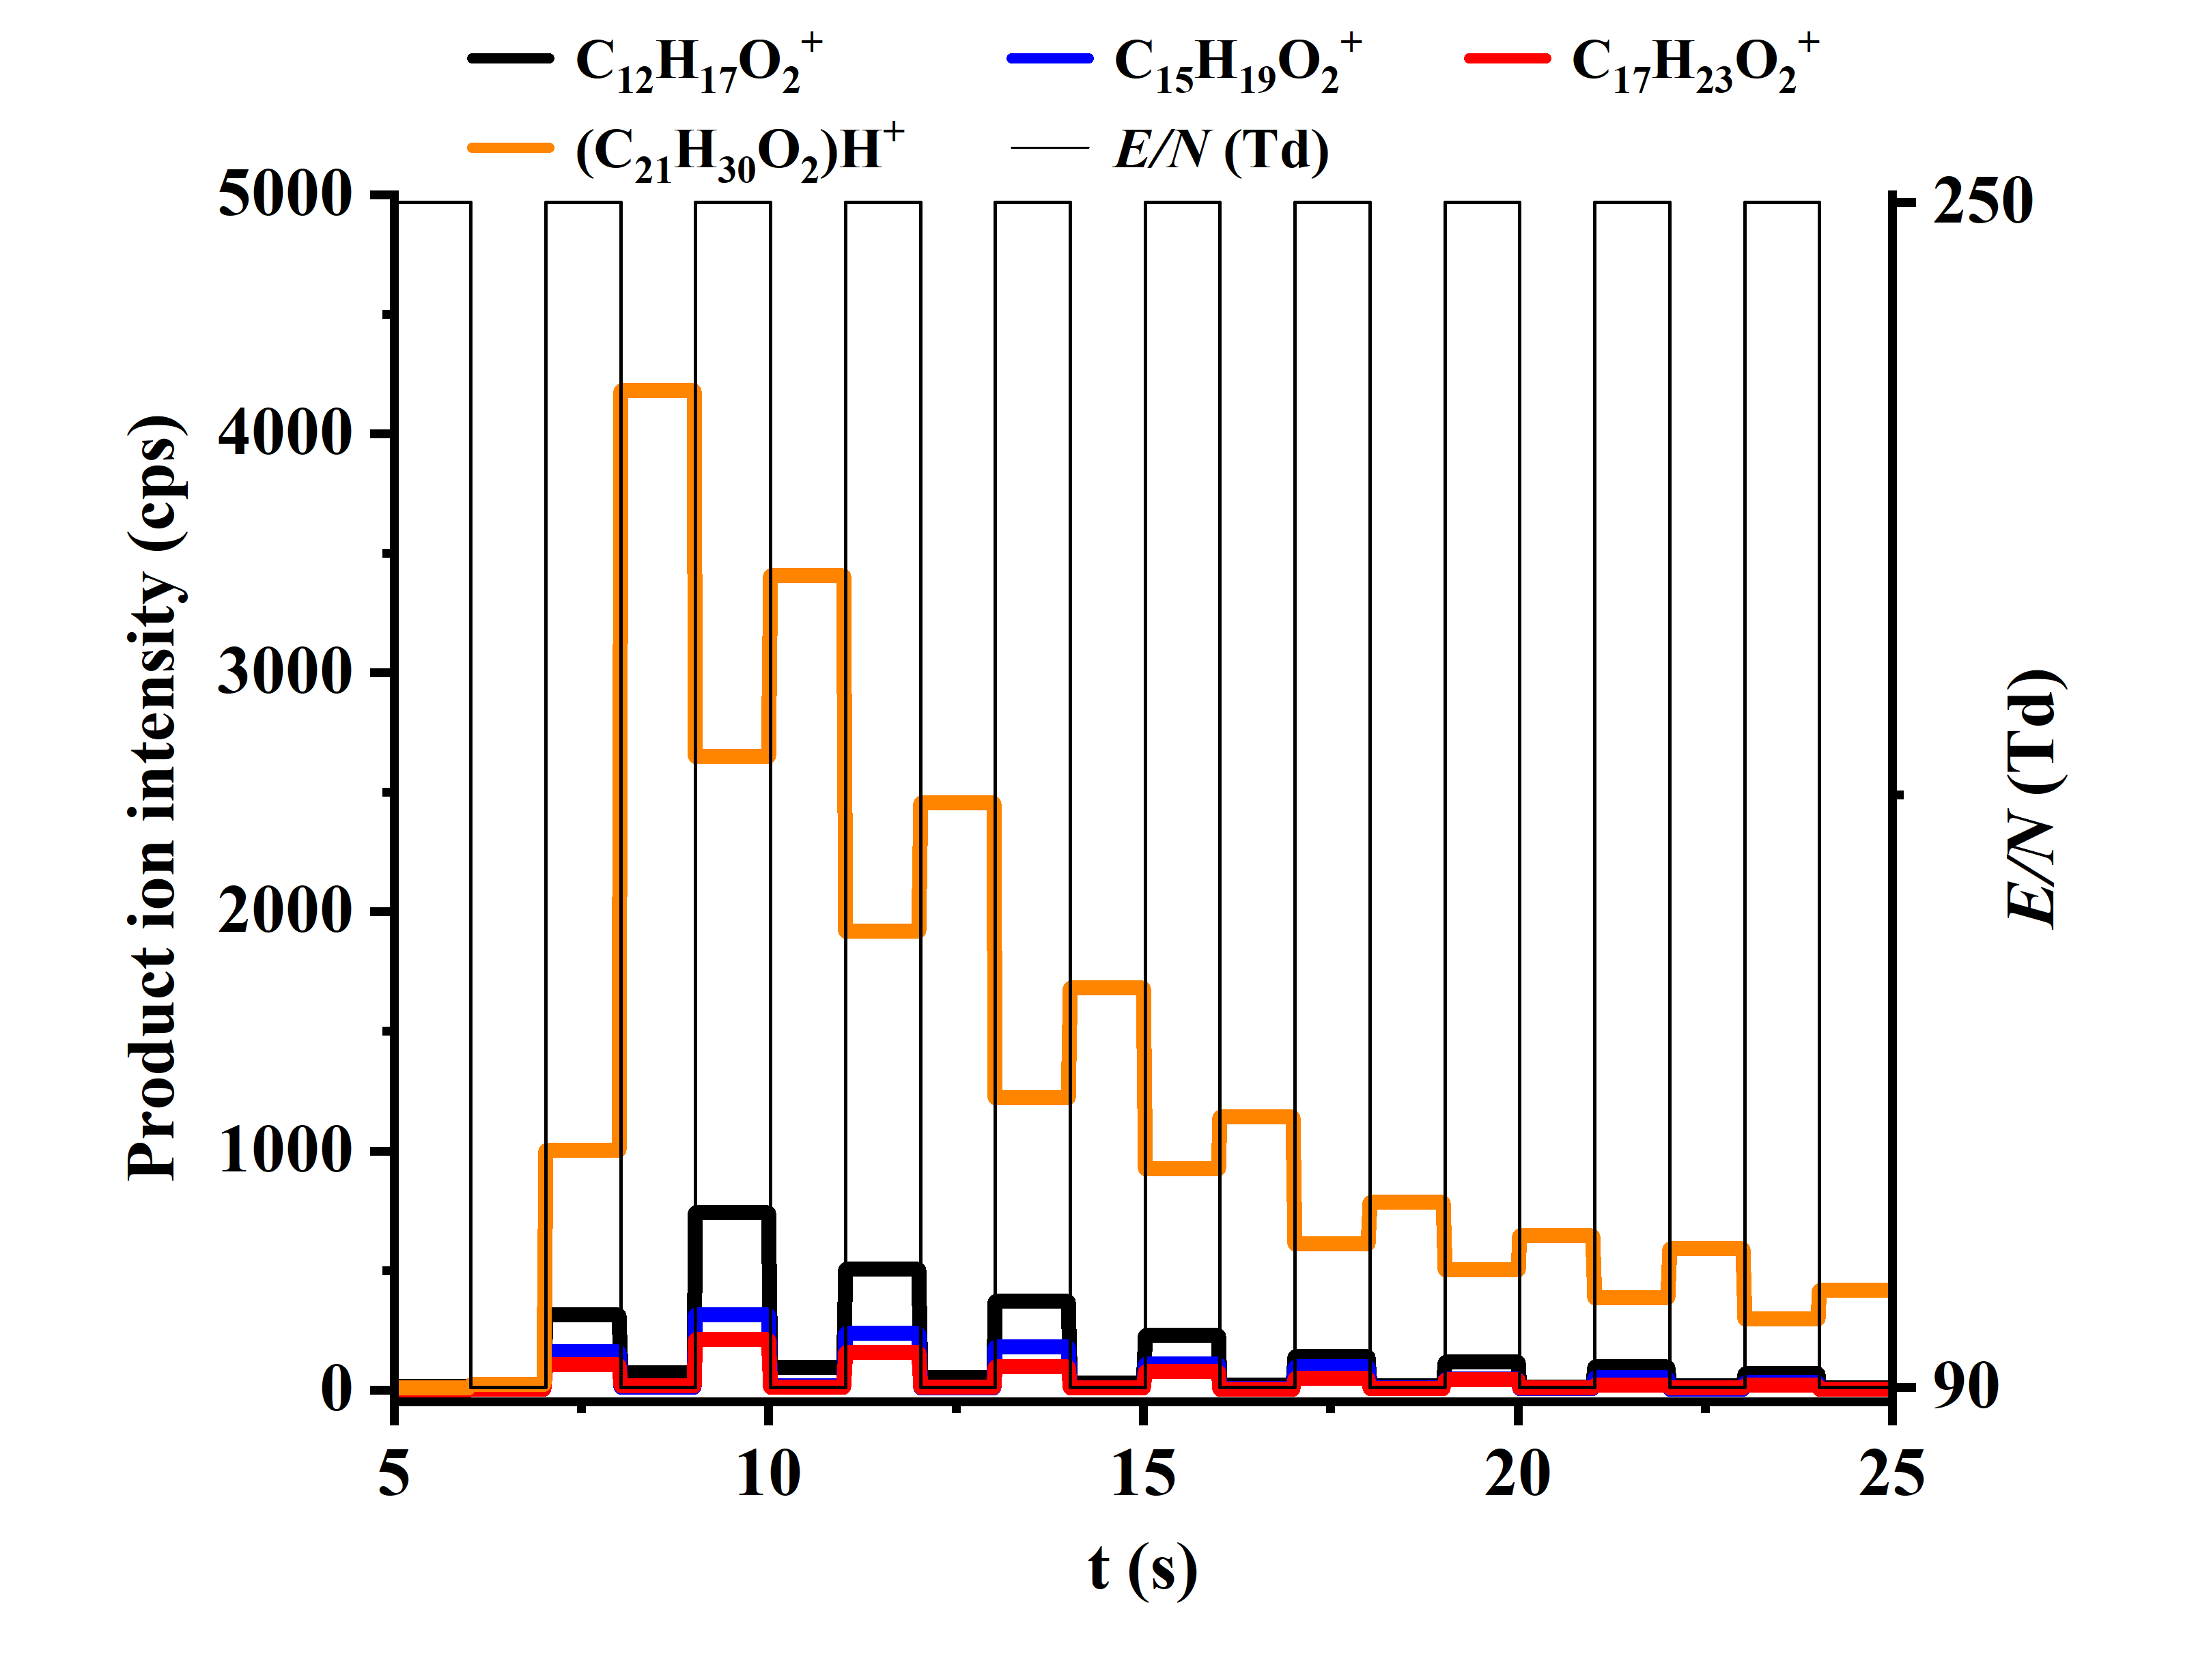
\includegraphics[width=0.45\textwidth]{pics/CBD-raw2.png}}
\caption[Example plots of data analysed with the fast-switching software]{Example plots of data analysed with the fast-switching software. Left: (a) raw and (c) averaged plots of H$_3$O$^+$ and (H$_2$O)H$_3$O$^+$ for the fast switching between 90 and 180 Td. Right: (b) raw and (d) averaged plots of the signal obtained from the desorption of trace amounts of cannabidiol while fast switching the reduced electric field between 90 and 250 Td.}
\label{fig:fss_plots}
\end{figure}


\subsection{Density functional theory}
Experimental data in this thesis is in some cases accompanied by theoretical values of the proton affinity, gas-phase basicity and energetics of the protonation and/or fragmentation reactions.
These density functional theory (\acrshort{dft}) results were computed   by Dr Peter Watts using  
Gaussian09W and GaussView05 for Windows  and the B3LYP functional with the 6-31+G(d,p) basis set  \cite{frisch2009gaussian}.

%\subsubsection{Saturation: Poisson distribution}

%The counting electronics in the PTR-ToF-MS assumes that each pulse measured at the MCP corresponds to one ion. This can be not true if two or more ions arrive at the detector very close together and their analogue signals overlap so that the TDC translates it as a single event. This is known as saturation and happens more often when a high concentration of a compound is being measured.

%At a given m/z, the maximum number of counts per second the instrument can measure corresponds to the number of cycles per second of the mass spectrometer, which is the number of times the ions are pulsed per second. In other words, at a certain \textit{m/z} only one ion per cycle can be measured. Therefore, a compromise must be found when the experiment is being designed to avoid situations of saturation while getting a proper signal. The number of cycles is the inverse of the cycle time, which is usually 30 to 40 us. For example, for a cycle time of 30 us, the number of cycles per second is 33333, or in other words, the pulsing frequency is 33.333 kHz.

%\autoref{fig:sat} shows the difference in real and measured counts if the probability of two ions arriving at the detector at the same time is given by the Poisson distribution function and considering that saturation means more than one ion arriving at the same time. When we are measuring a number of events equal to the number of cycles per second is unlikely that only one ion is arriving at the detector at a time, and the signal is highly saturated.

%The analytical expression is:
%\begin{equation}
%\label{eq:sat}
%P(x) = 1 - e^{-x}
%\end{equation}


%\begin{figure}%[ht]
%\centering
%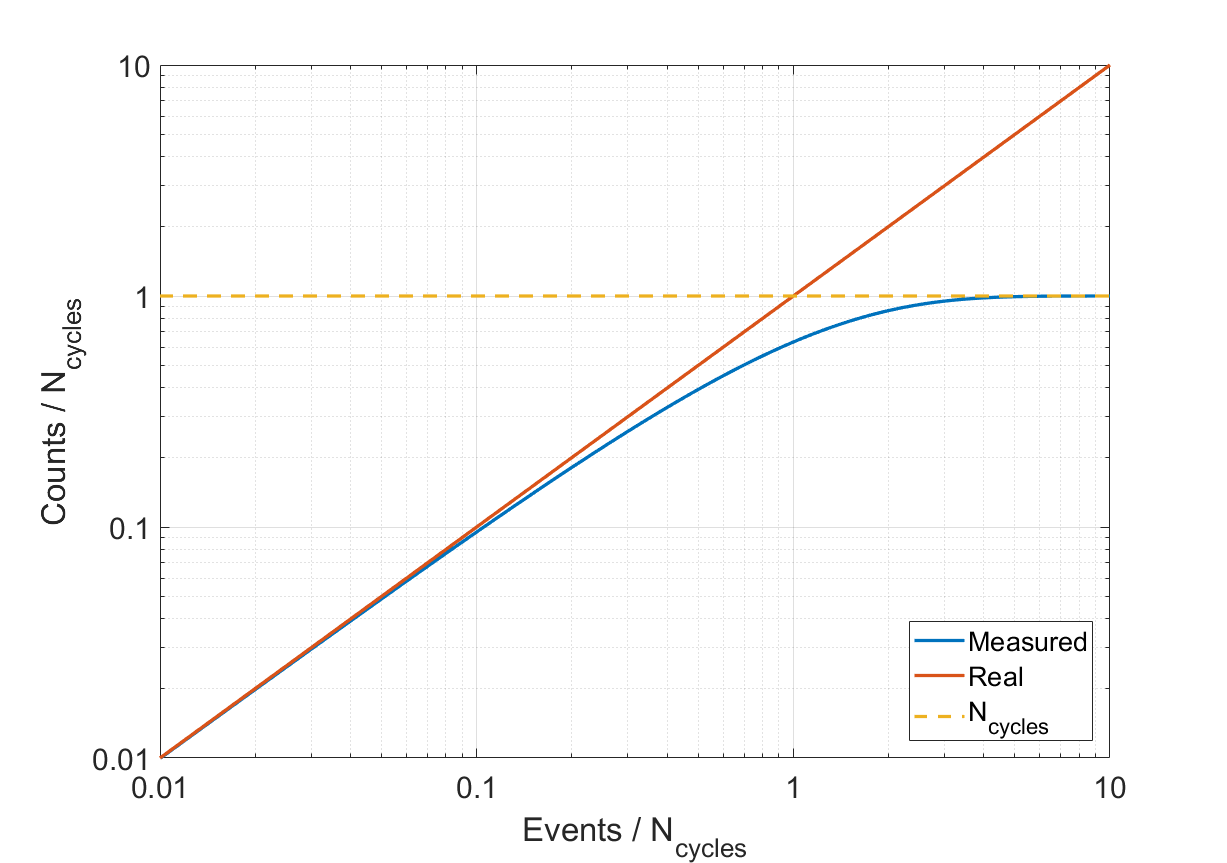
\includegraphics[width=0.8\linewidth]{pics/saturation.png}
%\centering
%\caption[Plot of the measured and real counts as a function of the number of events per cycle of the mass spectrometer.]{Plot of the measured (blue) and real (red) counts as a function of the number of events per cycle of the mass spectrometer. The dashed line corresponds to the number of cycles per second and indicates the maximum possible measured counts. Note that this plot is normalised to the number of cycles per second.}
%\label{fig:sat}
%\end{figure}




\section{PTR-MS Add-ons}
%\section{PTR-MS add-ons and latest hardware developments}
Besides the essential components described  earlier in this chapter, there are some accessories that can be coupled to a PTR-MS instrument for different purposes.
These include devices  like the CHARON real-time aerosol inlet  or the PREFICS pre concentrator with chromatographic separation \cite{muller2017direct,piel2019airborne,prefics}.
The ones included in this section are those used at some point for the experimental work in this thesis.




\subsection{Thermal Desorption Unit}\label{section:tdu}
For many applications, PTR-MS has been demonstrated to be a sensitive tool, yet the primary method for homeland security applications is \acrshort{ims}.
%
Most substances of relevance in this sector, including drugs and explosives, as well as in other fields have a small vapour pressure at room temperature, which challenges their identification. These are often referred to as semi-volatile organic compounds (\acrshort{svoc}s).
%
The sampling method is then critical in the detection of traces ammounts of these substances.


This issue has been approached in many interesting ways.
%
These include the patents for hand-held suction systems capable of identifying small quantities of explosives that were granted to \citeauthor{conrad1992hand} and to \citeauthor{carroll1992hand} \cite{conrad1992hand,carroll1992hand}.
%
\citeauthor{jjunju2015hand} also created a portable tool to detect nitroaromatic explosives on-site via atmospheric pressure chemical ionisation that can operate for 12 h in one charge \cite{jjunju2015hand}.
%
Additionally, the development of a biomimetic electronic dog nose by \citeauthor{staymates2016biomimetic} is an exciting new development \cite{staymates2016biomimetic}.
%Similar approaches to that mentioned here are taken by \citeauthor{ebejer2005rapid} \cite{ebejer2005rapid}



Swab desorptions are commonly used in  IMS  and the same approach can be brought into PTR-MS.
%
A thermal desorption unit (\acrshort{tdu})  like that engineered by KORE Technology Ltd  can be used to study SVOCs when coupled to a PTR-MS device (\autoref{fig:tdu}).
%
This was applied by \citeauthor{RN445} to the detection of explosives %reaching limits of detection (\acrshort{lod}) of nanograms  
and by \citeauthor{blenkhorn2019novel} to the detection polyaromatic hydrocarbons \cite{RN445,blenkhorn2019novel}.
%
This TDU works with polytetrafluoroethylene (\acrshort{ptfe}) swabs (ThermoFisher Scientific, Cheshire, UK) mounted in a cardboard frame (shown in \autoref{fig:tdu}a) onto which the targeted compounds are deposited.
%
Then, the swab is inserted in the TDU, whose plates come together clamping the swab and creating a high-quality circular seal. The metal plates are kept at high temperature (150$^{\circ}$C) and a carrier gas is flown through their holes, pulling the analyte towards the inlet pipe, whose surfaces are passivated (treated with SilcoNert\textsuperscript{\textregistered} 2000) to minimise adsorption.
%
This creates a desorption profile like the one in \autoref{fig:tdu_heroin}, where the two main fragment ions from trace amounts of the desorption of heroin are shown.
%
The duration of the desorption depends on many factors, being some of them the volatility of the analyte, the temperature of the inlet and TDU and the carrier gas flow.
%
It usually takes between 60 and 120 seconds for a sample to be completely desorbed into the instrument after the swab has been inserted in the TDU and its jaws have clamped together. After the measurement is finished, the TDU can be opened to extract the swab, which can be reused.







%\cite{koretdu}

\begin{figure}%[t]
  \sidesubfloat[]{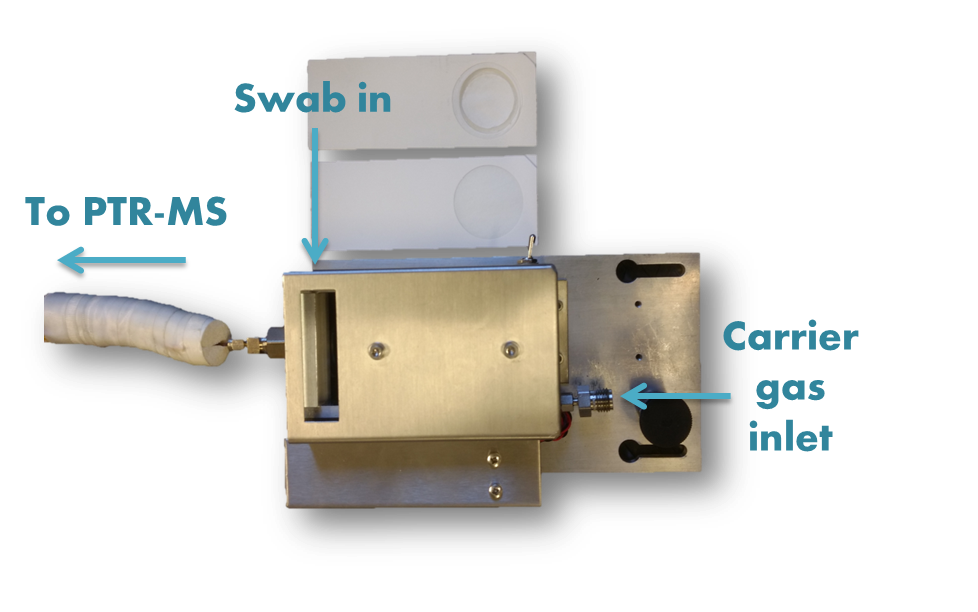
\includegraphics[width=0.7\linewidth]{pics/tdu.png}\label{fig:tdu1}}\\
  \sidesubfloat[]{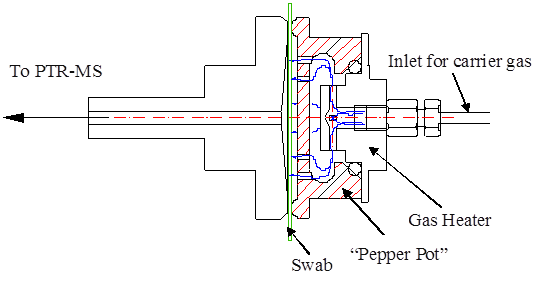
\includegraphics[width=0.7\linewidth]{pics/tdu2.png}\label{fig:tdu2}}
  \caption{(a) Picture of the TDU near to (top) used and (bottom) new PTFE swabs. (b) Schematic diagram of the TDU \cite{RN445}.}\label{fig:tdu}
\end{figure}

\begin{figure}%[t]
  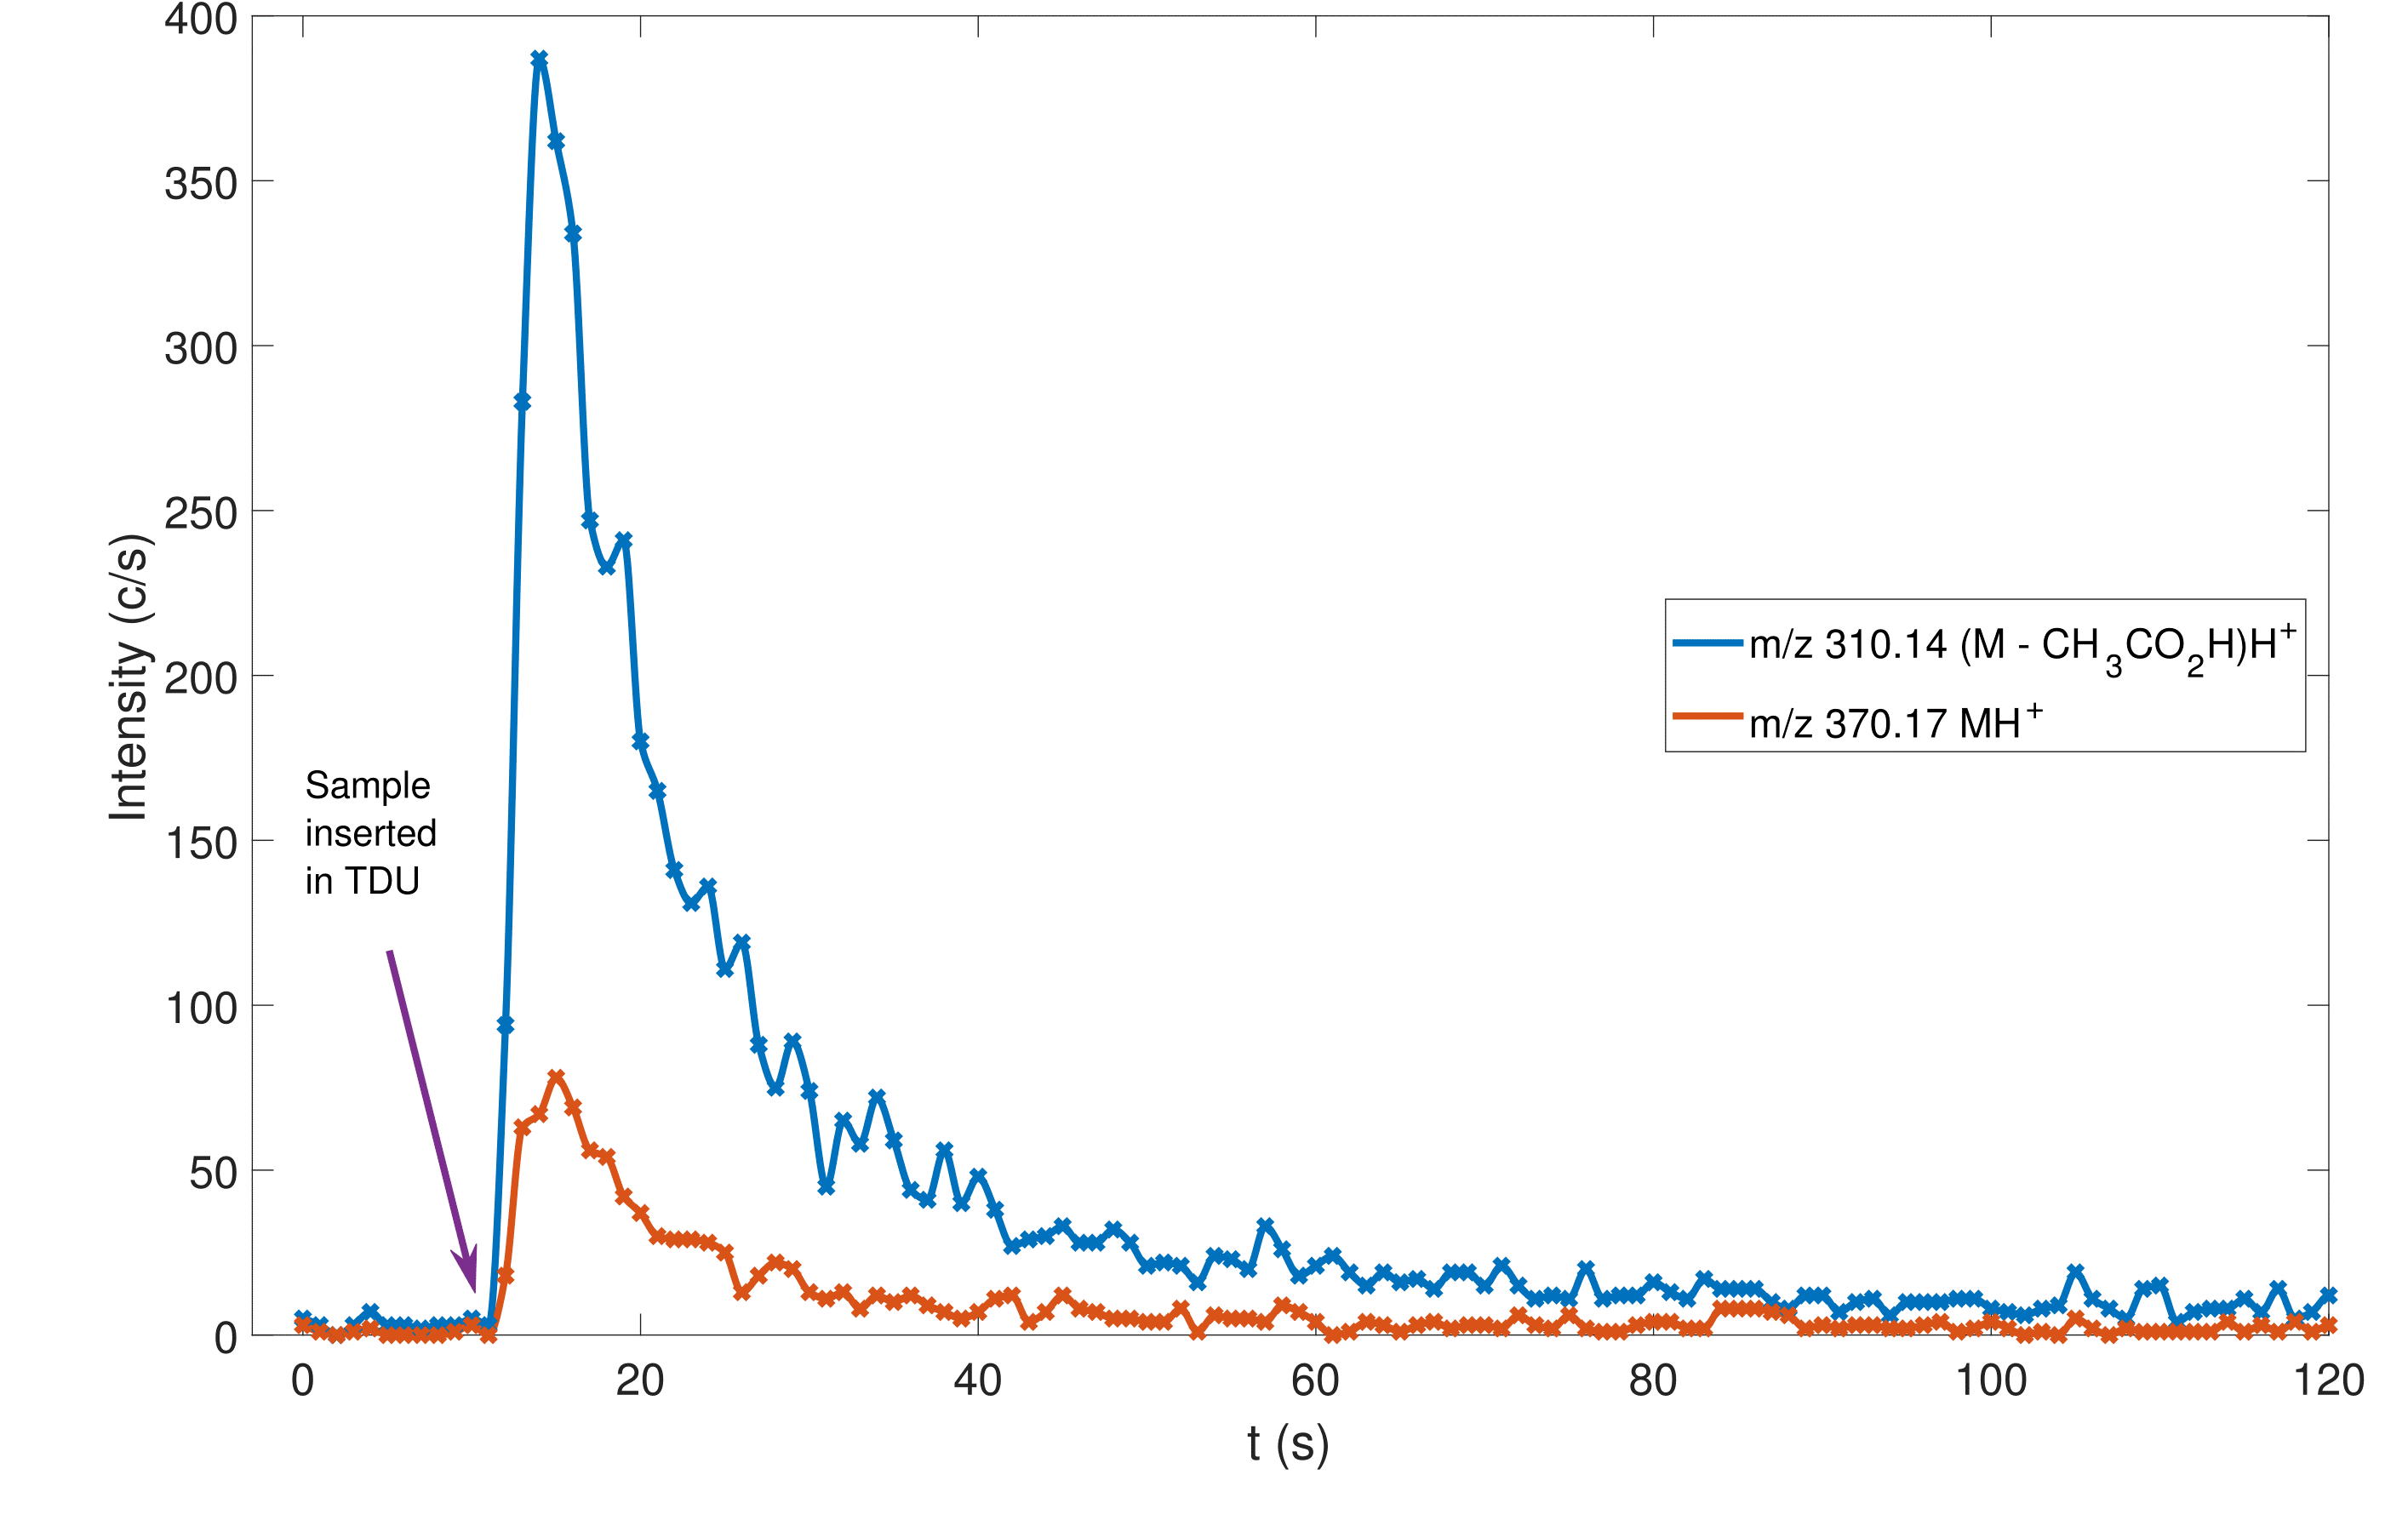
\includegraphics[width=0.7\linewidth]{pics/heroin_desorption.png}
  \caption{Time profiles of the count rates of two characteristic product ions at \textit{m/z} 310 and \textit{m/z} 370 during the thermal desorption of trace amounts of heroin at 120 Td using the TDU in PTR-MS.}\label{fig:tdu_heroin}
\end{figure}



\subsection{FastGC}\label{section:fastgc}

The fastGC (IONICON Analytik GmbH, Austria) is an add-on that aids in the product ion identification process by separating the analyte molecule from possible contaminants and impurities.

The working principle of the fastGC is the same as that of gas chromatography (\acrshort{gc}) systems, where
%
the components of a  gas mixture (mobile phase) present different retention times when flowing through a liquid or solid (stationary phase) packed inside a capillary column, which  separates them temporarily.
%
This separated mixture can be then injected into an analytical instrument for compound identification, where ion peaks occurring at the same retention time as the parent ion correspond to product ions.
%
The main differences between  GC and fastGC are that GC columns are tens of meters long, while fastGC ones are  10 meters long or less, and
%
also that the heating ramp in fastGC  is up to forty times faster than in conventional GC systems.
%
These characteristics make possible to perform a fastGC analysis in few minutes.



The fastGC was used in conjunction with a PTR-ToF 8000 (IONICON Analytik GmbH, Austria) to study the reactions of several ketones with H$_3$O$^+$ \cite{malaskova2019compendium}.
This add-on was used to ease the ion identification as the purity of the ketones was in the range 97 - 99\% and also decomposition of the sample could have occurred during storage.
%
This fastGC  is a modification of that used by \citeauthor{ruzsanyi2013multi} and \citeauthor{romano2014wine} \cite{ruzsanyi2013multi,romano2014wine}. Therefore only the differences with those will be briefly described here.
%
%The ketones were first introduced into a 0.5 ml sample loop  of passivated stainless steel.
%
The stationary phase in our system was a MXT-1 column (10 m × 0.53 mm, film thickness 0.25 µm, dimethyl polysiloxane phase, Restek, USA), which was heated from room temperature up to 240$^{\circ}$C in  2 minutes and 40 seconds.
%
Also, a 10-port passivated valve (VICI AG, Switzerland) and a three-way gas valve made from polyether ether ketone (\acrshort{peek}) replaced the four three-way valves and  needle valve in the previous design.
%
All sections of the inlet system are mounted in the oven which houses the drift tube to avoid cold spots.
%
This updated configuration allowed the sample loop to be constantly filled and the capillary column to be constantly back-flushing with the carrier gas.
%
The  carrier gas and make-up gas flows used were  8 ml/min and 20 ml/min of 6.0 N$_2$.







% this is literal from the article

%A custom-made valve block consisting of four three-way valves and a needle valve has been replaced by a 10-port passivated valve (VICI AG, Switzerland) and a three-way gas valve made from polyether ether ketone (\acrshort{peek}) was used.
%All parts of the inlet system are installed within the oven that houses the drift tube to prevent cold spots.
%This revised setup enabled constant filling of the sample loop and constant back- flushing of the capillary column with the carrier gas.
%8 ml/min and 20 ml/min of 6.0 N2 were used as carrier gas and make-up gas, respectively.


%A voltage ramp of 0.5 V/s from 10V up to 80V was applied raising the temperature of the capillary column reaching up to 240$^{\circ}$ from room temperature at a rate of up to 20$^{\circ}$C/second.































\subsection{Liquid Calibration Unit}\label{section:lcu}
The liquid calibration unit (\acrshort{lcu}, IONICON Analytik GmbH, Austria) %\citeauthor{ioniconlcu}, Austria)
is a standalone device that can be coupled to trace gas analysers for calibration purposes
where liquid standards are evaporated into a gas stream to yield known trace concentrations. % of the liquid.

%The main components of the LCU (\citeauthor{ioniconlcu}, Austria) are the nebuliser and the evaporation chamber.
The working principle of the LCU  has been explained in detail by \citeauthor{fischerlcu} \cite{fischerlcu}.
%
The  liquid sample is pumped from its container by a liquid flow controller into the nebuliser (X175, Burgener Research\textsuperscript{\textregistered}), where it mixes with the carrier gas (N$_2$ or zero air).
%
The nebulisation process creates a stream of micro-droplets that is then injected into the evaporation chamber.
%
This chamber is held at 100$^{\circ}$C to continue the process of evaporation, leading in a continuous flow of a known trace gas dilution that is then injected through a heated sampling line into the analytical instrument.

The LCU was used to study the reactions of several ketones with H$_3$O$^+$ in humid conditions \cite{malaskova2019compendium}.
This add-on was not used to calibrate the instrument but to create a steady signal of ketones samples in humid conditions. % at 100\% relative humidity at 37$^{\circ}$C.
%The one used in this study was manufactured by \citeauthor{ioniconlcu} and it has been explained in detail by \citeauthor{fischerlcu} \cite{fischerlcu}.
%
The sampling vials, kept at 30$^{\circ}$C, contained  trace quantities of  ketones  diluted in 100 ml of purified water and were  connected to the liquid inlet of the LCU. The liquid sample flow was of 35 µl/min, which with the carrier gas (N$_2$) flow of 950 ml/min gave an absolute humidity of 5\%.
%








